\documentclass[]{book}
\usepackage{lmodern}
\usepackage{amssymb,amsmath}
\usepackage{ifxetex,ifluatex}
\usepackage{fixltx2e} % provides \textsubscript
\ifnum 0\ifxetex 1\fi\ifluatex 1\fi=0 % if pdftex
  \usepackage[T1]{fontenc}
  \usepackage[utf8]{inputenc}
\else % if luatex or xelatex
  \ifxetex
    \usepackage{mathspec}
  \else
    \usepackage{fontspec}
  \fi
  \defaultfontfeatures{Ligatures=TeX,Scale=MatchLowercase}
\fi
% use upquote if available, for straight quotes in verbatim environments
\IfFileExists{upquote.sty}{\usepackage{upquote}}{}
% use microtype if available
\IfFileExists{microtype.sty}{%
\usepackage{microtype}
\UseMicrotypeSet[protrusion]{basicmath} % disable protrusion for tt fonts
}{}
\usepackage[a4paper, headheight=0pt, margin=0.75in]{geometry}
\usepackage{hyperref}
\hypersetup{unicode=true,
            pdftitle={R code for Robust soil mapping at the farm scale with vis-NIR spectroscopy (Ramirez-Lopez et al., 2019)},
            pdfauthor={Leo Ramirez-Lopez (BUCHI Labortechnik AG, Switzerland); Alex Wadoux (Wageningen University, Netherlands)},
            pdfborder={0 0 0},
            breaklinks=true}
\urlstyle{same}  % don't use monospace font for urls
\usepackage{natbib}
\bibliographystyle{apalike}
\usepackage{color}
\usepackage{fancyvrb}
\newcommand{\VerbBar}{|}
\newcommand{\VERB}{\Verb[commandchars=\\\{\}]}
\DefineVerbatimEnvironment{Highlighting}{Verbatim}{commandchars=\\\{\}}
% Add ',fontsize=\small' for more characters per line
\usepackage{framed}
\definecolor{shadecolor}{RGB}{248,248,248}
\newenvironment{Shaded}{\begin{snugshade}}{\end{snugshade}}
\newcommand{\AlertTok}[1]{\textcolor[rgb]{0.94,0.16,0.16}{#1}}
\newcommand{\AnnotationTok}[1]{\textcolor[rgb]{0.56,0.35,0.01}{\textbf{\textit{#1}}}}
\newcommand{\AttributeTok}[1]{\textcolor[rgb]{0.77,0.63,0.00}{#1}}
\newcommand{\BaseNTok}[1]{\textcolor[rgb]{0.00,0.00,0.81}{#1}}
\newcommand{\BuiltInTok}[1]{#1}
\newcommand{\CharTok}[1]{\textcolor[rgb]{0.31,0.60,0.02}{#1}}
\newcommand{\CommentTok}[1]{\textcolor[rgb]{0.56,0.35,0.01}{\textit{#1}}}
\newcommand{\CommentVarTok}[1]{\textcolor[rgb]{0.56,0.35,0.01}{\textbf{\textit{#1}}}}
\newcommand{\ConstantTok}[1]{\textcolor[rgb]{0.00,0.00,0.00}{#1}}
\newcommand{\ControlFlowTok}[1]{\textcolor[rgb]{0.13,0.29,0.53}{\textbf{#1}}}
\newcommand{\DataTypeTok}[1]{\textcolor[rgb]{0.13,0.29,0.53}{#1}}
\newcommand{\DecValTok}[1]{\textcolor[rgb]{0.00,0.00,0.81}{#1}}
\newcommand{\DocumentationTok}[1]{\textcolor[rgb]{0.56,0.35,0.01}{\textbf{\textit{#1}}}}
\newcommand{\ErrorTok}[1]{\textcolor[rgb]{0.64,0.00,0.00}{\textbf{#1}}}
\newcommand{\ExtensionTok}[1]{#1}
\newcommand{\FloatTok}[1]{\textcolor[rgb]{0.00,0.00,0.81}{#1}}
\newcommand{\FunctionTok}[1]{\textcolor[rgb]{0.00,0.00,0.00}{#1}}
\newcommand{\ImportTok}[1]{#1}
\newcommand{\InformationTok}[1]{\textcolor[rgb]{0.56,0.35,0.01}{\textbf{\textit{#1}}}}
\newcommand{\KeywordTok}[1]{\textcolor[rgb]{0.13,0.29,0.53}{\textbf{#1}}}
\newcommand{\NormalTok}[1]{#1}
\newcommand{\OperatorTok}[1]{\textcolor[rgb]{0.81,0.36,0.00}{\textbf{#1}}}
\newcommand{\OtherTok}[1]{\textcolor[rgb]{0.56,0.35,0.01}{#1}}
\newcommand{\PreprocessorTok}[1]{\textcolor[rgb]{0.56,0.35,0.01}{\textit{#1}}}
\newcommand{\RegionMarkerTok}[1]{#1}
\newcommand{\SpecialCharTok}[1]{\textcolor[rgb]{0.00,0.00,0.00}{#1}}
\newcommand{\SpecialStringTok}[1]{\textcolor[rgb]{0.31,0.60,0.02}{#1}}
\newcommand{\StringTok}[1]{\textcolor[rgb]{0.31,0.60,0.02}{#1}}
\newcommand{\VariableTok}[1]{\textcolor[rgb]{0.00,0.00,0.00}{#1}}
\newcommand{\VerbatimStringTok}[1]{\textcolor[rgb]{0.31,0.60,0.02}{#1}}
\newcommand{\WarningTok}[1]{\textcolor[rgb]{0.56,0.35,0.01}{\textbf{\textit{#1}}}}
\usepackage{longtable,booktabs}
\usepackage{graphicx,grffile}
\makeatletter
\def\maxwidth{\ifdim\Gin@nat@width>\linewidth\linewidth\else\Gin@nat@width\fi}
\def\maxheight{\ifdim\Gin@nat@height>\textheight\textheight\else\Gin@nat@height\fi}
\makeatother
% Scale images if necessary, so that they will not overflow the page
% margins by default, and it is still possible to overwrite the defaults
% using explicit options in \includegraphics[width, height, ...]{}
\setkeys{Gin}{width=\maxwidth,height=\maxheight,keepaspectratio}
\IfFileExists{parskip.sty}{%
\usepackage{parskip}
}{% else
\setlength{\parindent}{0pt}
\setlength{\parskip}{6pt plus 2pt minus 1pt}
}
\setlength{\emergencystretch}{3em}  % prevent overfull lines
\providecommand{\tightlist}{%
  \setlength{\itemsep}{0pt}\setlength{\parskip}{0pt}}
\setcounter{secnumdepth}{5}
% Redefines (sub)paragraphs to behave more like sections
\ifx\paragraph\undefined\else
\let\oldparagraph\paragraph
\renewcommand{\paragraph}[1]{\oldparagraph{#1}\mbox{}}
\fi
\ifx\subparagraph\undefined\else
\let\oldsubparagraph\subparagraph
\renewcommand{\subparagraph}[1]{\oldsubparagraph{#1}\mbox{}}
\fi

%%% Use protect on footnotes to avoid problems with footnotes in titles
\let\rmarkdownfootnote\footnote%
\def\footnote{\protect\rmarkdownfootnote}

%%% Change title format to be more compact
\usepackage{titling}

% Create subtitle command for use in maketitle
\providecommand{\subtitle}[1]{
  \posttitle{
    \begin{center}\large#1\end{center}
    }
}

\setlength{\droptitle}{-2em}

  \title{R code for Robust soil mapping at the farm scale with vis-NIR spectroscopy (Ramirez-Lopez \emph{et al.}, 2019)}
    \pretitle{\vspace{\droptitle}\centering\huge}
  \posttitle{\par}
    \author{Leo Ramirez-Lopez (BUCHI Labortechnik AG, Switzerland) \\ Alex Wadoux (Wageningen University, Netherlands)}
    \preauthor{\centering\large\emph}
  \postauthor{\par}
      \predate{\centering\large\emph}
  \postdate{\par}
    \date{* First Published: 2019-06-18 * * Updated: 2019-06-20 *}

\usepackage{booktabs}
\usepackage{amsthm}
\makeatletter
\def\thm@space@setup{%
  \thm@preskip=8pt plus 2pt minus 4pt
  \thm@postskip=\thm@preskip
}
\makeatother

\begin{document}
\maketitle

{
\setcounter{tocdepth}{1}
\tableofcontents
}
\hypertarget{preface}{%
\chapter*{Preface}\label{preface}}
\addcontentsline{toc}{chapter}{Preface}

In the spirit of reproducible research, here we share the data and the computational code
used for carrying out the analyses presented in our paper \href{https://onlinelibrary.wiley.com/doi/10.1111/ejss.12752}{``Robust soil mapping at the farm scale with vis-NIR spectroscopy''} which is by the way open access. Before you go thorugh this code we strongly recoment to read our paper.

\begin{figure}
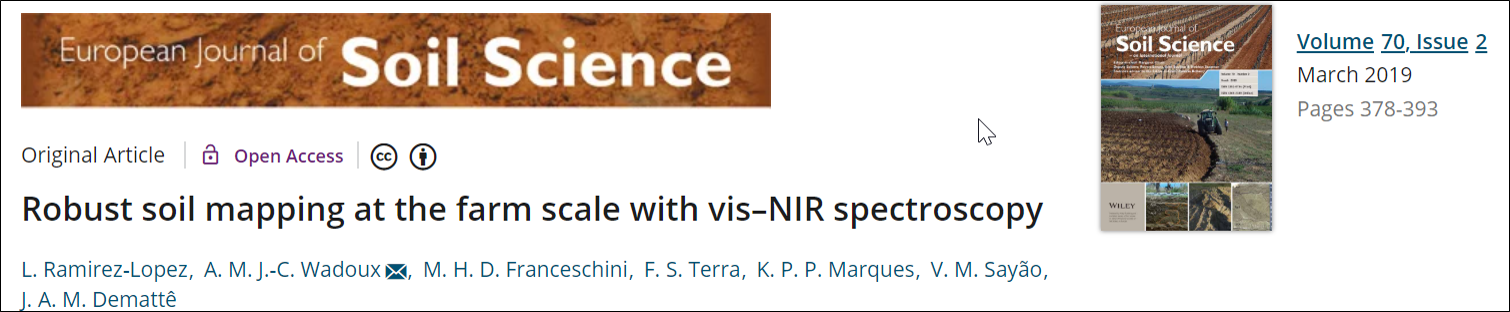
\includegraphics[width=0.9\linewidth]{./maps/paperimg} \end{figure}

\hypertarget{intro}{%
\chapter{Introduction}\label{intro}}

Here you will find some basic informatzion about the paper and the \texttt{R} code opresented here.

\hypertarget{paper-summary}{%
\section{Paper summary}\label{paper-summary}}

Sustainable agriculture practices are often hampered by the prohibitive costs associated with the generation of fine-resolution soil maps. Recently, several papers have been published highlighting how visible and near infrared(vis-NIR) reflectance spectroscopy may offer an alternative to address this problem by increasing the density of soil sampling and by reducing the number of conventional laboratory analyses needed. However, for farm-scale soil mapping, previous studies rarely focused on sample optimization for the calibration of vis-NIR models or on robust modelling of the spatial variation of soil properties predicted by vis-NIR spectroscopy. In the present study, we used soil vis-NIR spectroscopy models optimized in terms of both number of calibration samples and accuracy for high-resolution robust farm-scale soil mapping and addressed some of the most common pitfalls identified in previous research. We collected 910 samples from 458 locations at two depths (A, 0-0.20 m; B, 0.80-1.0 m) in the state of Sao Paulo, Brazil. All soil samples were analysed by conventional methods and scanned in the vis-NIR spectral range. With the vis-NIR spectra only, we inferred statistically the optimal set size and the best samples with which to calibrate vis-NIR models. The calibrated vis-NIR models were validated and used to predict soil properties for the rest of the samples. The prediction error of the spectroscopic model was propagated through the spatial analysis, in which robust block kriging was used to predict particle-size fractions and exchangeable calcium content for each depth. The results indicated that statistical selection of the calibration samples based on vis-NIR spectra considerably decreased the need for conventional chemical analysis for a given level of mapping accuracy.

\hypertarget{study-area}{%
\section{Study area}\label{study-area}}

The study area is located in Brazil between the municipalities of Barra Bonita and Mineiros do Tiete (in the state of Sao Paulo).

\hypertarget{htmlwidget-4a8fbaf5c5d6d8b2878c}{}

\label{fig:unnamed-chunk-2}View of the study area

\hypertarget{in-case-of-commentsquestionsissues}{%
\section{In case of comments/questions/issues}\label{in-case-of-commentsquestionsissues}}

In case you have any question comments/questions/issue related to the code presented here please go to:\\
\url{https://github.com/l-ramirez-lopez/VNIR_spectroscopy_for_robust_soil_mapping/issues} and create a new issue.

\hypertarget{for-citation-or-details-please-refer-to}{%
\section{For citation or details please refer to:}\label{for-citation-or-details-please-refer-to}}

Ramirez-Lopez, L., Wadoux, A. C., Franceschini, M. H. D., Terra, F. S., Marques, K. P. P., Sayao, V. M., \& Dematte, J. A. M. (2019). \href{https://onlinelibrary.wiley.com/doi/10.1111/ejss.12752}{Robust soil mapping at the farm scale with vis-NIR spectroscopy}. European Journal of Soil Science.

\hypertarget{notes}{%
\section{Notes}\label{notes}}

\begin{itemize}
\item
  \emph{Reproducibility}: slight discrepancies between the results of reoported in the paper and the results you get in your \texttt{R} console might be expected in case you use different \texttt{R} package versions and different random number generators.
\item
  \emph{To advanced R users}: In order to make the \texttt{R} code more readable/interpretable we have opted for using \texttt{for} loops instead of vectorized functions. There are several aspects of the code that can be improved to reach better computational efficiency.
\end{itemize}

\hypertarget{required-r-packages}{%
\chapter{\texorpdfstring{Required \texttt{R} packages}{Required R packages}}\label{required-r-packages}}

In order to run all the code presented in the next sections you will need to have the following packages installed

\begin{center}\rule{0.5\linewidth}{\linethickness}\end{center}

You can install the required packages using the following code

\begin{Shaded}
\begin{Highlighting}[]
\NormalTok{requiredpackages <-}\StringTok{ }\KeywordTok{c}\NormalTok{(}\StringTok{"resemble"}\NormalTok{, }\StringTok{"prospectr"}\NormalTok{, }\StringTok{"clhs"}\NormalTok{, }\StringTok{"matrixStats"}\NormalTok{, }\StringTok{"doParallel"}\NormalTok{, }
                    \StringTok{"ggplot2"}\NormalTok{, }\StringTok{"tidyr"}\NormalTok{, }\StringTok{"tidyverse"}\NormalTok{, }\StringTok{"georob"}\NormalTok{, }\StringTok{"rgdal"}\NormalTok{, }\StringTok{"raster"}\NormalTok{, }\StringTok{"RColorBrewer"}\NormalTok{)}
\NormalTok{toinstall <-}\StringTok{ }\NormalTok{requiredpackages[}\OperatorTok{!}\NormalTok{requiredpackages }\OperatorTok\StringTok{ }\KeywordTok{rownames}\NormalTok{(}\KeywordTok{installed.packages}\NormalTok{())]}
\ControlFlowTok{if}\NormalTok{ (}\KeywordTok{length}\NormalTok{(toinstall) }\OperatorTok{>}\StringTok{ }\DecValTok{0}\NormalTok{) \{}
                    \KeywordTok{install.packages}\NormalTok{(toinstall)}
\NormalTok{\}}
\KeywordTok{lapply}\NormalTok{(requiredpackages, }\DataTypeTok{FUN =}\NormalTok{ library, }\DataTypeTok{character.only =} \OtherTok{TRUE}\NormalTok{)}
\end{Highlighting}
\end{Shaded}

\hypertarget{required-data}{%
\chapter{Required data}\label{required-data}}

In this section you will find the instructions on how to download and read the soil dataset used in our paper.

\begin{center}\rule{0.5\linewidth}{\linethickness}\end{center}

You can download the file \href{https://github.com/l-ramirez-lopez/VNIR_spectroscopy_for_robust_soil_mapping/raw/master/SoilNIRSaoPaulo.rds}{`SoilNIRSaoPaulo.rds'}, alternatively you can visit to the \href{https://github.com/l-ramirez-lopez/VNIR_spectroscopy_for_robust_soil_mapping}{GitHub repository of the paper} where the file resides.

This \texttt{rds} file contains a \texttt{data.frame} with 910 rows (samples) and the following variables:

\begin{itemize}
\tightlist
\item
  Nr: An arbitrary sample number.
\item
  ID: A \texttt{factor} indicating the sample IDs. The first character is a letter which indicates the depth layer at which the sample was collected (A: 0-20 cm and B: 80-100 cm).\\
\item
  POINT\_X: The X (geographical) coordinate.
\item
  POINT\_Y: The Y (geographical) coordinate.
\item
  Sand: The percentage of sand contnet in the soil sample.
\item
  Silt: The percentage of silt contnet in the soil sample.
\item
  Clay: The percentage of clay contnet in the soil sample.
\item
  Ca: The exchangeable Calcium content in the sample (\(mmol_{c}\) \(kg^{−1}\)).
\item
  set: A \texttt{factor} indicating whether the sample is used for model's validation or if it can be used to calibrate models.
\item
  spc: A set of 307 variables representing the wavelengths from 502 nm to 2338 nm in steps of 6 nm.
\end{itemize}

Further information on this dataset can be found in \href{https://onlinelibrary.wiley.com/doi/epdf/10.1111/ejss.12752}{our paper}

We recommend to create a local folder (e.g.~``./myworkingdirectory''). If you downloaded the file to this local folder then:

\begin{Shaded}
\begin{Highlighting}[]
\NormalTok{workingd <-}\StringTok{ "/myworkingdirectory"}
\KeywordTok{setwd}\NormalTok{(workingd)}
\NormalTok{data <-}\StringTok{ }\KeywordTok{readRDS}\NormalTok{(}\StringTok{"SoilNIRSaoPaulo.rds"}\NormalTok{)}
\end{Highlighting}
\end{Shaded}

Alternatively, you can also read the file directly from the \href{https://github.com/l-ramirez-lopez/VNIR_spectroscopy_for_robust_soil_mapping}{GitHub repository of the paper}:

\begin{Shaded}
\begin{Highlighting}[]
\NormalTok{nirfile <-}\StringTok{ }\KeywordTok{file}\NormalTok{(}\StringTok{"https://github.com/l-ramirez-lopez/VNIR_spectroscopy_for_robust_soil_mapping/raw/master/SoilNIRSaoPaulo.rds"}\NormalTok{)}
\NormalTok{data <-}\StringTok{ }\KeywordTok{readRDS}\NormalTok{(nirfile)}
\KeywordTok{names}\NormalTok{(data)}
\end{Highlighting}
\end{Shaded}

\begin{verbatim}
##  [1] "Nr"      "ID"      "POINT_X" "POINT_Y" "Sand"    "Silt"    "Clay"   
##  [8] "Ca"      "set"     "spc"
\end{verbatim}

Plot the spectra of the loaded data..

\begin{Shaded}
\begin{Highlighting}[]
\NormalTok{obg <-}\StringTok{ }\KeywordTok{par}\NormalTok{()}\OperatorTok{$}\NormalTok{bg}
\KeywordTok{par}\NormalTok{(}\DataTypeTok{bg =} \KeywordTok{rgb}\NormalTok{(}\FloatTok{0.11}\NormalTok{, }\FloatTok{0.12}\NormalTok{, }\FloatTok{0.17}\NormalTok{))}
\NormalTok{tcol <-}\StringTok{ }\KeywordTok{rgb}\NormalTok{(}\FloatTok{0.6}\NormalTok{, }\FloatTok{0.6}\NormalTok{, }\FloatTok{0.6}\NormalTok{, }\FloatTok{0.8}\NormalTok{)}
\NormalTok{scol <-}\StringTok{ }\KeywordTok{rgb}\NormalTok{(}\DecValTok{0}\NormalTok{, }\DecValTok{1}\NormalTok{, }\DecValTok{0}\NormalTok{, }\FloatTok{0.2}\NormalTok{)}
\KeywordTok{matplot}\NormalTok{(}\DataTypeTok{x =} \KeywordTok{as.numeric}\NormalTok{(}\KeywordTok{colnames}\NormalTok{(data}\OperatorTok{$}\NormalTok{spc)), }\DataTypeTok{y =} \KeywordTok{t}\NormalTok{(data}\OperatorTok{$}\NormalTok{spc), }\DataTypeTok{type =} \StringTok{"l"}\NormalTok{, }\DataTypeTok{lty =} \DecValTok{1}\NormalTok{, }
                    \DataTypeTok{col =}\NormalTok{ scol, }\DataTypeTok{xlab =} \StringTok{"wavelength (nm)"}\NormalTok{, }\DataTypeTok{ylab =} \StringTok{"Absorbance"}\NormalTok{, }\DataTypeTok{col.axis =}\NormalTok{ tcol, }
                    \DataTypeTok{col.lab =}\NormalTok{ tcol)}
\KeywordTok{grid}\NormalTok{(}\DataTypeTok{lty =} \DecValTok{1}\NormalTok{, }\DataTypeTok{col =}\NormalTok{ tcol)}
\end{Highlighting}
\end{Shaded}

\begin{figure}
\centering
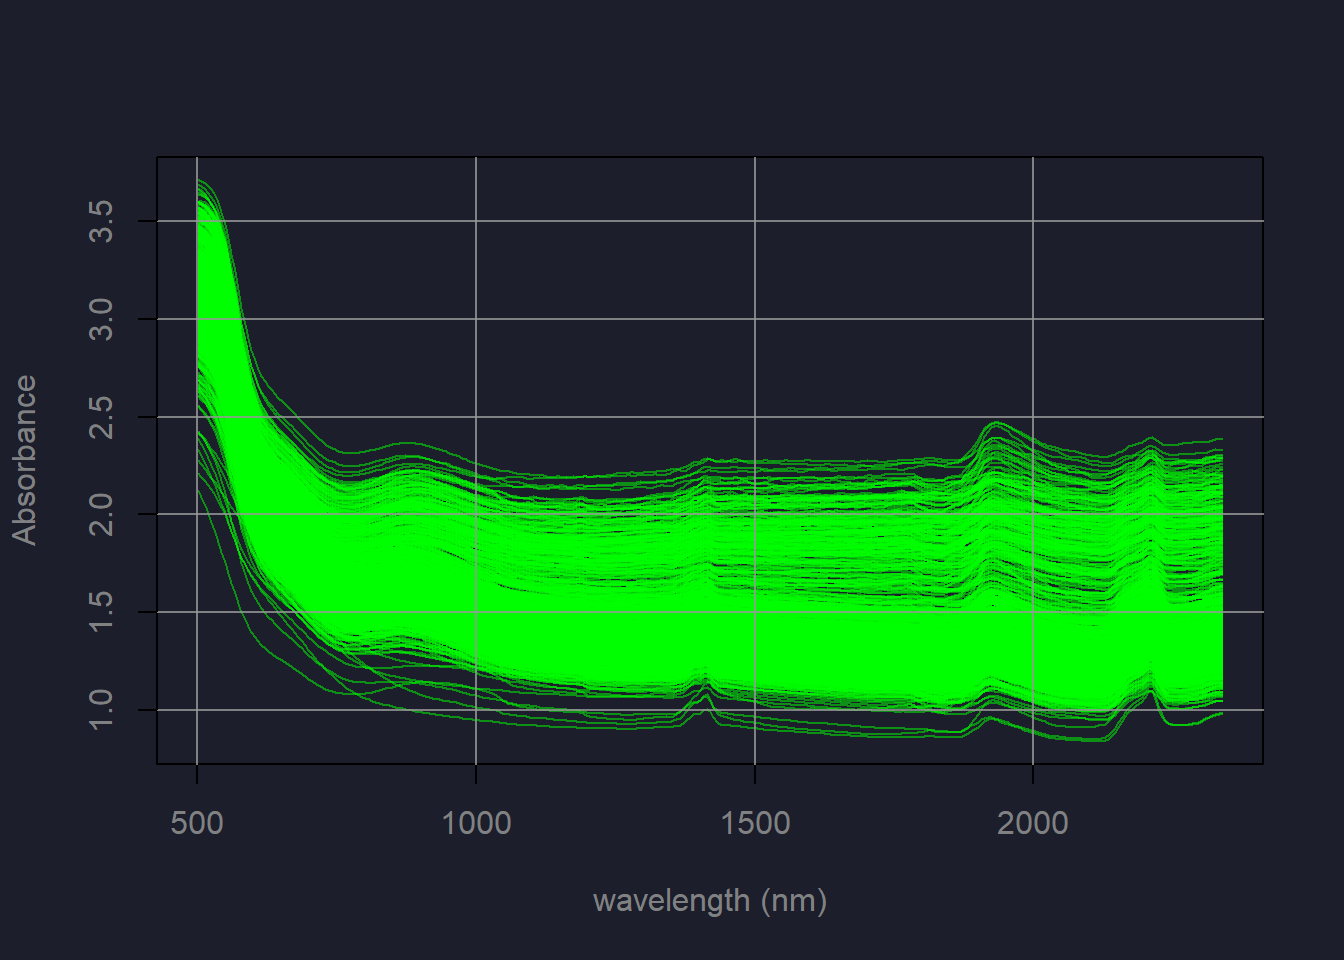
\includegraphics{soilmappingwithvnir_files/figure-latex/unnamed-chunk-5-1.pdf}
\caption{\label{fig:unnamed-chunk-5}Spectra in the SoilNIRSaoPaulo dataset}
\end{figure}

\begin{Shaded}
\begin{Highlighting}[]
\CommentTok{## reset the background color of your plots to the original color}
\KeywordTok{par}\NormalTok{(}\DataTypeTok{bg =}\NormalTok{ obg)}
\end{Highlighting}
\end{Shaded}

In addition you also need a \texttt{R} object of class (\texttt{SpatialPolygonsDataFrame} of the package \texttt{sp}) which contains the polygon of the study area. You can also download the file (polygon.rds) containing this object by clicking \href{https://github.com/l-ramirez-lopez/VNIR_spectroscopy_for_robust_soil_mapping/raw/master/polygon.rds}{here}.

\hypertarget{sampling}{%
\chapter{Sampling}\label{sampling}}

\begin{center}\rule{0.5\linewidth}{\linethickness}\end{center}

\hypertarget{optimal-calibration-set-size-identification}{%
\section{Optimal calibration set size identification}\label{optimal-calibration-set-size-identification}}

In this section we show how the optimal size for a calibration set is identified using the mean squared
Euclidean distance (\(msd\)) between estimates of the probability density functions (\(pdfs\)) of the whole set of samples and the pdfs of subsets with different sizes.\\
First we compute the principal components (PCs) of the NIR spectra of the whole set of calibration candidate samples. Then for each component we compute kernel density estimates (\(KDE\)):

\begin{Shaded}
\begin{Highlighting}[]
\CommentTok{## Apply standard normal variate }
\NormalTok{data}\OperatorTok{$}\NormalTok{spc_snv <-}\StringTok{ }\KeywordTok{standardNormalVariate}\NormalTok{(data}\OperatorTok{$}\NormalTok{spc)}

\CommentTok{## extract the validation samples into a new set/object}
\NormalTok{valida <-}\StringTok{ }\NormalTok{data[data}\OperatorTok{$}\NormalTok{set }\OperatorTok{==}\StringTok{ "validation"}\NormalTok{,]}

\CommentTok{## remove the validation samples from data}
\NormalTok{data <-}\StringTok{ }\NormalTok{data[data}\OperatorTok{$}\NormalTok{set }\OperatorTok{==}\StringTok{ "cal_candidate"}\NormalTok{,]}

\CommentTok{## --- 2. Perform a principal component analysis  ----}
\CommentTok{## Compress the data }
\NormalTok{pcaall <-}\StringTok{ }\KeywordTok{orthoProjection}\NormalTok{(}\DataTypeTok{Xr =}\NormalTok{ data}\OperatorTok{$}\NormalTok{spc_snv, }
                          \DataTypeTok{X2 =} \OtherTok{NULL}\NormalTok{, }
                          \DataTypeTok{Yr =} \OtherTok{NULL}\NormalTok{, }
                          \DataTypeTok{method =} \StringTok{"pca"}\NormalTok{, }
                          \DataTypeTok{pcSelection =} \KeywordTok{list}\NormalTok{(}\StringTok{"cumvar"}\NormalTok{, }\FloatTok{0.99}\NormalTok{), }
                          \DataTypeTok{center =} \OtherTok{TRUE}\NormalTok{, }
                          \DataTypeTok{scaled =} \OtherTok{FALSE}\NormalTok{)}
                          
\CommentTok{## standardize the socres}
\NormalTok{pcaall}\OperatorTok{$}\NormalTok{scores.std <-}\StringTok{ }\KeywordTok{sweep}\NormalTok{(pcaall}\OperatorTok{$}\NormalTok{scores, }\DataTypeTok{MARGIN =} \DecValTok{2}\NormalTok{, }\DataTypeTok{STATS =}\NormalTok{ pcaall}\OperatorTok{$}\NormalTok{sc.sdv, }\DataTypeTok{FUN =} \StringTok{"/"}\NormalTok{)}

\CommentTok{## compute the max and min of each score for the limits of the density estimations}
\NormalTok{max.sc <-}\StringTok{ }\KeywordTok{colMins}\NormalTok{(pcaall}\OperatorTok{$}\NormalTok{scores.std)}
\NormalTok{min.sc <-}\StringTok{ }\KeywordTok{colMaxs}\NormalTok{(pcaall}\OperatorTok{$}\NormalTok{scores.std)}

\CommentTok{## compute the mean and sd of each score for the comparisons with the samples}
\NormalTok{mean.sc <-}\StringTok{ }\KeywordTok{colMeans}\NormalTok{(pcaall}\OperatorTok{$}\NormalTok{scores.std)}
\NormalTok{sd.sc <-}\StringTok{ }\KeywordTok{colSds}\NormalTok{(pcaall}\OperatorTok{$}\NormalTok{scores.std)}

\CommentTok{# number of points in the density distribution}
\NormalTok{nxdens <-}\StringTok{ }\DecValTok{500}

\CommentTok{## matrix where the density values will be stored}
\NormalTok{ix <-}\StringTok{ }\DecValTok{1}
\NormalTok{sc.dens <-}\StringTok{ }\KeywordTok{data.frame}\NormalTok{(}\KeywordTok{seq}\NormalTok{(min.sc[ix], max.sc[ix], }\DataTypeTok{length =}\NormalTok{ nxdens), }
                      \KeywordTok{matrix}\NormalTok{(}\OtherTok{NA}\NormalTok{, nxdens, }\KeywordTok{length}\NormalTok{(min.sc)))}
\KeywordTok{colnames}\NormalTok{(sc.dens) <-}\StringTok{ }\KeywordTok{c}\NormalTok{(}\StringTok{"x"}\NormalTok{, }\KeywordTok{paste}\NormalTok{(}\StringTok{"densc"}\NormalTok{, }\DecValTok{1}\OperatorTok{:}\KeywordTok{length}\NormalTok{(min.sc), }\DataTypeTok{sep =} \StringTok{""}\NormalTok{))}

\CommentTok{## Kernel density estimates (KDE) of each component }
\NormalTok{d.bandwidths <-}\StringTok{ }\KeywordTok{rep}\NormalTok{(}\OtherTok{NA}\NormalTok{, }\KeywordTok{length}\NormalTok{(min.sc))}
\KeywordTok{names}\NormalTok{(d.bandwidths) <-}\StringTok{ }\KeywordTok{colnames}\NormalTok{(pcaall}\OperatorTok{$}\NormalTok{scores.std)}
\ControlFlowTok{for}\NormalTok{(i }\ControlFlowTok{in} \DecValTok{1}\OperatorTok{:}\KeywordTok{length}\NormalTok{(min.sc))\{}
\NormalTok{  idsty <-}\StringTok{ }\KeywordTok{density}\NormalTok{(pcaall}\OperatorTok{$}\NormalTok{scores.std[,i], }
                   \DataTypeTok{bw =} \StringTok{"nrd0"}\NormalTok{, }
                   \DataTypeTok{n =}\NormalTok{ nxdens, }\DataTypeTok{from =}\NormalTok{ min.sc[i], }\DataTypeTok{to =}\NormalTok{ max.sc[i], }
                   \DataTypeTok{kernel =} \StringTok{"gaussian"}\NormalTok{)}
\NormalTok{  sc.dens[,i}\OperatorTok{+}\DecValTok{1}\NormalTok{] <-}\StringTok{ }\NormalTok{idsty}\OperatorTok{$}\NormalTok{y}
\NormalTok{  d.bandwidths[i] <-}\StringTok{ }\NormalTok{idsty}\OperatorTok{$}\NormalTok{bw}
\NormalTok{\}}

\CommentTok{## Create the vector of different sample set sizes to be tested}
\NormalTok{css <-}\StringTok{ }\KeywordTok{seq}\NormalTok{(}\DecValTok{10}\NormalTok{, }\DecValTok{400}\NormalTok{, }\DataTypeTok{by =} \DecValTok{10}\NormalTok{)}
\end{Highlighting}
\end{Shaded}

Now we will iterate over the different calibration set sizes (\texttt{css}). We are going to use the LHS algorithm to select subsets from our set of candiate samples for calibartion. This is done using the (standardized) scores of the principal components (PCs) of the spectra (\texttt{pcaall\$scores.std}). For each calibration subset we'll compute the mean squared Euclidean distance (\(msd\)) between estimates of the probability density functions (\(pdfs\)) of the whole set of samples and the \(pdfs\) of samples in the subset. The \(msd\) is computed using kernel density estimates (\(KDE\)) of the \(pdfs\). To obtain reliable estimates of \(msd\) as a function of the sample set size, we will repeat 10 times (\texttt{repetitions}) the whole sampling procedure for each \texttt{css}, the final \(msd\) will be the the average of the \(msd\)s obtained at each iteration.
The following pseudo-code summarizes the procedure to compute the \(msd\) (see the `\emph{Calibration samples}' section in our paper for more details):

\begin{verbatim}
Input:  PCs of the whole set of candidate samples (p);
        KDEs of the PCs of the whole set of candidate samples;
Output: msd

1 for each repetition do:
2   for each proposed sampling size do:
3     select from the PCs a subset (s);
4     for each component in s and p:
5       compute the msd between KDE(s,component) and KDE(p,component);
6     end
7   end
8 end

9 aggregate the results of the msds obatined for all 
the repetition iterations for each sample set size
\end{verbatim}

First we'll compute the \(msd\)s for ecah repetition and we will write each set of results into our working directory.

\begin{Shaded}
\begin{Highlighting}[]
\CommentTok{## Sample with LHS (latin hypercube sampling)}

\CommentTok{## These three nested loops might take a while}
\CommentTok{## (aprox. 16 min per repetition, i.e. a bit more than a couple of hours }
\CommentTok{## for the whole thing)}
\CommentTok{## (for reducing the computation time the loops}
\CommentTok{## can be vectorized using the apply family of functions. }
\CommentTok{## Furtheromre parallelization of the loop for the repetitions}
\CommentTok{## can also be applied)}
\CommentTok{## We present the computations with nested loops for interpretability }
\CommentTok{## reasons}

\NormalTok{repetitions <-}\StringTok{ }\DecValTok{10}

\CommentTok{## root name for the results of each iteration}
\NormalTok{filerootname <-}\StringTok{ "6pcs_resultsclhs_rep"}

\CommentTok{## Create the data.frame where the results will be stored }
\CommentTok{## at each iteration}
\NormalTok{results.clhs <-}\StringTok{  }\KeywordTok{data.frame}\NormalTok{(}\DataTypeTok{css =}\NormalTok{ css, }
                            \DataTypeTok{msd =} \KeywordTok{rep}\NormalTok{(}\OtherTok{NA}\NormalTok{, }\KeywordTok{length}\NormalTok{(css)),}
                            \DataTypeTok{mndiff =} \KeywordTok{rep}\NormalTok{(}\OtherTok{NA}\NormalTok{, }\KeywordTok{length}\NormalTok{(css)),}
                            \DataTypeTok{sddiff =} \KeywordTok{rep}\NormalTok{(}\OtherTok{NA}\NormalTok{, }\KeywordTok{length}\NormalTok{(css)))}
\ControlFlowTok{for}\NormalTok{(k }\ControlFlowTok{in} \DecValTok{1}\OperatorTok{:}\NormalTok{repetitions)\{}
\NormalTok{  results.clhs[,}\OperatorTok{-}\DecValTok{1}\NormalTok{] <-}\StringTok{ }\OtherTok{NA}
  
  \CommentTok{## Define a file name}
\NormalTok{  fn <-}\StringTok{ }\KeywordTok{paste}\NormalTok{(filerootname, k,}\StringTok{".txt"}\NormalTok{, }\DataTypeTok{sep =} \StringTok{""}\NormalTok{)}
  \ControlFlowTok{if}\NormalTok{(fn }\OperatorTok\StringTok{ }\KeywordTok{list.files}\NormalTok{())\{}
\NormalTok{    results.clhs <-}\StringTok{ }\KeywordTok{read.table}\NormalTok{(fn, }\DataTypeTok{header =}\NormalTok{ T, }\DataTypeTok{sep =} \StringTok{"}\CharTok{\textbackslash{}t}\StringTok{"}\NormalTok{)}
\NormalTok{  \}}
  
\NormalTok{  iter.p <-}\StringTok{ }\DecValTok{1} \OperatorTok{+}\StringTok{ }\KeywordTok{sum}\NormalTok{(}\KeywordTok{rowSums}\NormalTok{(}\OperatorTok{!}\KeywordTok{is.na}\NormalTok{(results.clhs)) }\OperatorTok{==}\StringTok{ }\KeywordTok{ncol}\NormalTok{(results.clhs))}
  
  \ControlFlowTok{for}\NormalTok{(i }\ControlFlowTok{in}\NormalTok{ iter.p}\OperatorTok{:}\KeywordTok{length}\NormalTok{(css))\{}
    \KeywordTok{set.seed}\NormalTok{(k)}
\NormalTok{    i.calidx <-}\StringTok{ }\KeywordTok{clhs}\NormalTok{(}\DataTypeTok{x =} \KeywordTok{as.data.frame}\NormalTok{(pcaall}\OperatorTok{$}\NormalTok{scores.std),}
                     \DataTypeTok{size =}\NormalTok{ css[i], }
                     \DataTypeTok{iter =} \DecValTok{10000}\NormalTok{)}
    
    \CommentTok{## Compute the KDEs of each PC}
\NormalTok{    j.sc.dens <-}\StringTok{ }\NormalTok{msd.sc  <-}\StringTok{ }\NormalTok{sc.dens }
    \ControlFlowTok{for}\NormalTok{(j }\ControlFlowTok{in} \DecValTok{1}\OperatorTok{:}\KeywordTok{length}\NormalTok{(min.sc))\{}
      \CommentTok{## use the same bandwidth (bw) as in the whole set of candidates}
\NormalTok{      j.sc.dens[,j }\OperatorTok{+}\StringTok{ }\DecValTok{1}\NormalTok{] <-}\StringTok{ }\KeywordTok{density}\NormalTok{(}\DataTypeTok{x =}\NormalTok{ pcaall}\OperatorTok{$}\NormalTok{scores.std[i.calidx,j], }
                                   \DataTypeTok{bw =}\NormalTok{ d.bandwidths[j], }
                                   \DataTypeTok{n =}\NormalTok{ nxdens, }
                                   \DataTypeTok{from =}\NormalTok{ min.sc[j], }
                                   \DataTypeTok{to =}\NormalTok{ max.sc[j], }
                                   \DataTypeTok{kernel =} \StringTok{"gaussian"}\NormalTok{)}\OperatorTok{$}\NormalTok{y}
\NormalTok{    \}}
\NormalTok{    results.clhs}\OperatorTok{$}\NormalTok{msd[i] <-}\StringTok{ }\KeywordTok{mean}\NormalTok{(}\KeywordTok{colMeans}\NormalTok{((j.sc.dens[,}\OperatorTok{-}\DecValTok{1}\NormalTok{] }\OperatorTok{-}\StringTok{ }\NormalTok{sc.dens[,}\OperatorTok{-}\DecValTok{1}\NormalTok{])}\OperatorTok{^}\DecValTok{2}\NormalTok{, }\DataTypeTok{na.rm =}\NormalTok{ T))}
\NormalTok{    results.clhs}\OperatorTok{$}\NormalTok{mndiff[i] <-}\StringTok{ }\KeywordTok{mean}\NormalTok{(}\KeywordTok{abs}\NormalTok{(}\KeywordTok{colMeans}\NormalTok{(pcaall}\OperatorTok{$}\NormalTok{scores.std[i.calidx,])))}
\NormalTok{    results.clhs}\OperatorTok{$}\NormalTok{sddiff[i] <-}\StringTok{ }\KeywordTok{mean}\NormalTok{(}\KeywordTok{abs}\NormalTok{(}\KeywordTok{colSds}\NormalTok{(pcaall}\OperatorTok{$}\NormalTok{scores.std[i.calidx,]) }\OperatorTok{-}\StringTok{ }\DecValTok{1}\NormalTok{))}
    
    \CommentTok{## write the results obtained so far...}
    \ControlFlowTok{if}\NormalTok{(iter }\OperatorTok{==}\StringTok{ }\KeywordTok{length}\NormalTok{(nmsrepsclhs))\{}
\NormalTok{      final.clhs <-}\StringTok{ }\NormalTok{final.clhs}\OperatorTok{/}\NormalTok{iter}
      \KeywordTok{write.table}\NormalTok{(}\DataTypeTok{x =}\NormalTok{ final.clhs, }
                  \DataTypeTok{file =} \StringTok{"6pcs_final.clhs.txt"}\NormalTok{, }
                  \DataTypeTok{sep =} \StringTok{"}\CharTok{\textbackslash{}t}\StringTok{"}\NormalTok{, }
                  \DataTypeTok{row.names =} \OtherTok{FALSE}\NormalTok{)}
\NormalTok{    \}}
    
    \KeywordTok{print}\NormalTok{(results.clhs[}\DecValTok{1}\OperatorTok{:}\NormalTok{i,])}
\NormalTok{  \}}
\NormalTok{\}}
\end{Highlighting}
\end{Shaded}

After executing the above nested loops, you should have obtained 10 different *.txt files in your working directorty (in this case the root name of the files is 6pcs\_resultsclhs\_rep{[}n{]}.txt where {[}n{]} represents the repetition number). These files contain the \(msd\) results obtained at each repetition iteration.
Now we'll calculate the final \(msd\) as the average of the ones obtained at each repetition iteration.

\begin{Shaded}
\begin{Highlighting}[]
\CommentTok{## Specify a file name for the file where the final results will be stored}
\NormalTok{finalresultsfile <-}\StringTok{ "6pcs_final.clhs.txt"}

\NormalTok{nmsrepsclhs <-}\StringTok{ }\KeywordTok{paste}\NormalTok{(filerootname, }\DecValTok{1}\OperatorTok{:}\NormalTok{repetitions, }\StringTok{".txt"}\NormalTok{, }\DataTypeTok{sep =} \StringTok{""}\NormalTok{)}
\NormalTok{final.clhs <-}\StringTok{ }\DecValTok{0}
\ControlFlowTok{for}\NormalTok{(i }\ControlFlowTok{in}\NormalTok{ nmsrepsclhs)\{}
\NormalTok{  iter <-}\StringTok{ }\KeywordTok{which}\NormalTok{(i }\OperatorTok{==}\StringTok{ }\NormalTok{nmsrepsclhs)}
\NormalTok{  results.clhs <-}\StringTok{ }\KeywordTok{read.table}\NormalTok{(i, }\DataTypeTok{header =}\NormalTok{ T, }\DataTypeTok{sep =} \StringTok{"}\CharTok{\textbackslash{}t}\StringTok{"}\NormalTok{)}
\NormalTok{  results.clhs}\OperatorTok{$}\NormalTok{mndiff <-}\StringTok{ }\KeywordTok{abs}\NormalTok{(results.clhs}\OperatorTok{$}\NormalTok{mndiff)}
\NormalTok{  final.clhs <-}\StringTok{ }\NormalTok{final.clhs }\OperatorTok{+}\StringTok{ }\NormalTok{results.clhs}

  \CommentTok{## write a table with the final results }
  \ControlFlowTok{if}\NormalTok{(iter }\OperatorTok{==}\StringTok{ }\KeywordTok{length}\NormalTok{(nmsrepsclhs))\{}
\NormalTok{    final.clhs <-}\StringTok{ }\NormalTok{final.clhs}\OperatorTok{/}\NormalTok{iter}
    \KeywordTok{write.table}\NormalTok{(}\DataTypeTok{x =}\NormalTok{ final.clhs, }
                \DataTypeTok{file =}\NormalTok{ finalresultsfile, }
                \DataTypeTok{sep =} \StringTok{"}\CharTok{\textbackslash{}t}\StringTok{"}\NormalTok{, }
                \DataTypeTok{row.names =} \OtherTok{FALSE}\NormalTok{)}
\NormalTok{  \}}
\NormalTok{\}}

\CommentTok{## Compute the standard devitions of the msd results}
\NormalTok{final.clhs_sd <-}\StringTok{ }\DecValTok{0}
\ControlFlowTok{for}\NormalTok{(i }\ControlFlowTok{in}\NormalTok{ nmsrepsclhs)\{}
\NormalTok{  iter <-}\StringTok{ }\KeywordTok{which}\NormalTok{(i }\OperatorTok{==}\StringTok{ }\NormalTok{nmsrepsclhs)}
\NormalTok{  results.clhs <-}\StringTok{ }\KeywordTok{read.table}\NormalTok{(i, }\DataTypeTok{header =}\NormalTok{ T, }\DataTypeTok{sep =} \StringTok{"}\CharTok{\textbackslash{}t}\StringTok{"}\NormalTok{)}
\NormalTok{  results.clhs}\OperatorTok{$}\NormalTok{mndiff <-}\StringTok{ }\KeywordTok{abs}\NormalTok{(results.clhs}\OperatorTok{$}\NormalTok{mndiff)}
\NormalTok{  final.clhs_sd <-}\StringTok{ }\NormalTok{(results.clhs }\OperatorTok{-}\StringTok{ }\NormalTok{final.clhs_sd)}\OperatorTok{^}\DecValTok{2}
  \ControlFlowTok{if}\NormalTok{(iter }\OperatorTok{==}\StringTok{ }\KeywordTok{length}\NormalTok{(nmsrepsclhs))\{}
\NormalTok{    final.clhs_sd <-}\StringTok{ }\NormalTok{(final.clhs_sd}\OperatorTok{/}\NormalTok{iter)}\OperatorTok{^}\FloatTok{0.5}
\NormalTok{  \}}
\NormalTok{\}}
\end{Highlighting}
\end{Shaded}

After executing the above code, a file with the final \(msd\) estimations is writen in your working directory. In addition the standard deviations of the \(msd\) for the different set sizes was also computed and stored in the object \texttt{final.clhs\_sd}.

\hypertarget{plotting-the-results}{%
\section{Plotting the results}\label{plotting-the-results}}

To plot the \(msd\) results using \texttt{ggplot} (Figure 3 in our paper):

\begin{Shaded}
\begin{Highlighting}[]
\NormalTok{final.clhs_plot <-}\StringTok{ }\KeywordTok{data.frame}\NormalTok{(final.clhs[,}\DecValTok{1}\OperatorTok{:}\DecValTok{2}\NormalTok{], }
                              \DataTypeTok{sd_lower =}\NormalTok{ final.clhs[,}\DecValTok{2}\NormalTok{] }\OperatorTok{-}\StringTok{ }\NormalTok{final.clhs_sd[,}\DecValTok{2}\NormalTok{],}
                              \DataTypeTok{sd_upper =}\NormalTok{ final.clhs[,}\DecValTok{2}\NormalTok{] }\OperatorTok{+}\StringTok{ }\NormalTok{final.clhs_sd[,}\DecValTok{2}\NormalTok{])}

\NormalTok{p.tmp <-}\StringTok{ }\KeywordTok{ggplot}\NormalTok{(final.clhs_plot) }\OperatorTok{+}\StringTok{ }\KeywordTok{geom_line}\NormalTok{(}\KeywordTok{aes}\NormalTok{(}\DataTypeTok{x =}\NormalTok{ css, msd, }\DataTypeTok{colour =} \StringTok{"msd"}\NormalTok{)) }\OperatorTok{+}\StringTok{ }
\StringTok{  }\KeywordTok{theme_bw}\NormalTok{() }\OperatorTok{+}\StringTok{ }
\StringTok{  }\KeywordTok{theme}\NormalTok{(}\DataTypeTok{axis.title.y =} \KeywordTok{element_text}\NormalTok{(}\DataTypeTok{face=} \StringTok{"bold.italic"}\NormalTok{, }\DataTypeTok{colour =} \KeywordTok{grey}\NormalTok{(}\FloatTok{0.2}\NormalTok{), }\DataTypeTok{size=}\DecValTok{18}\NormalTok{),}
        \DataTypeTok{axis.text.y  =} \KeywordTok{element_text}\NormalTok{(}\DataTypeTok{angle=}\DecValTok{0}\NormalTok{, }\DataTypeTok{vjust =}\FloatTok{0.5}\NormalTok{, }\DataTypeTok{hjust =}\FloatTok{0.5}\NormalTok{, }\DataTypeTok{size=}\DecValTok{14}\NormalTok{), }
        \DataTypeTok{legend.title =} \KeywordTok{element_text}\NormalTok{(}\DataTypeTok{colour =} \StringTok{"white"}\NormalTok{, }\DataTypeTok{size=}\DecValTok{20}\NormalTok{)) }\OperatorTok{+}
\StringTok{  }\KeywordTok{theme}\NormalTok{(}\DataTypeTok{axis.title.x =} \KeywordTok{element_text}\NormalTok{(}\DataTypeTok{face=} \StringTok{"bold"}\NormalTok{, }\DataTypeTok{colour =} \KeywordTok{grey}\NormalTok{(}\FloatTok{0.2}\NormalTok{), }\DataTypeTok{size=}\DecValTok{18}\NormalTok{),}
        \DataTypeTok{axis.text.x  =} \KeywordTok{element_text}\NormalTok{(}\DataTypeTok{angle =} \DecValTok{0}\NormalTok{, }\DataTypeTok{vjust=}\DecValTok{0}\NormalTok{, }\DataTypeTok{size=}\DecValTok{14}\NormalTok{)) }\OperatorTok{+}
\StringTok{  }\KeywordTok{theme}\NormalTok{(}\DataTypeTok{legend.position =} \StringTok{"none"}\NormalTok{) }\OperatorTok{+}\StringTok{ }
\StringTok{  }\KeywordTok{theme}\NormalTok{(}\DataTypeTok{legend.text =} \KeywordTok{element_text}\NormalTok{(}\DataTypeTok{face=}\StringTok{"bold"}\NormalTok{, }\DataTypeTok{colour =} \KeywordTok{grey}\NormalTok{(}\FloatTok{0.2}\NormalTok{), }\DataTypeTok{size=}\DecValTok{18}\NormalTok{)) }\OperatorTok{+}
\StringTok{  }\KeywordTok{labs}\NormalTok{(}\DataTypeTok{y =} \StringTok{"msd"}\NormalTok{, }\DataTypeTok{x =} \StringTok{"Calibration set size"}\NormalTok{) }\OperatorTok{+}
\StringTok{  }\CommentTok{#coord_cartesian(ylim = c(0, 8)) + }
\StringTok{  }\KeywordTok{theme}\NormalTok{(}\DataTypeTok{strip.background =} \KeywordTok{element_rect}\NormalTok{(}\DataTypeTok{fill =} \StringTok{"grey"}\NormalTok{), }
        \DataTypeTok{strip.text.x =} \KeywordTok{element_text}\NormalTok{(}\DataTypeTok{size =} \DecValTok{16}\NormalTok{, }\DataTypeTok{colour =} \StringTok{"black"}\NormalTok{, }\DataTypeTok{angle =} \DecValTok{0}\NormalTok{)) }
        
\NormalTok{p.tmp }\OperatorTok{+}\StringTok{ }
\StringTok{  }\KeywordTok{geom_ribbon}\NormalTok{(}\KeywordTok{aes}\NormalTok{(}\DataTypeTok{ymin=}\NormalTok{sd_lower, }\DataTypeTok{ymax=}\NormalTok{sd_upper, }\DataTypeTok{x=}\NormalTok{css, }\DataTypeTok{colour =} \StringTok{"bands"}\NormalTok{), }\DataTypeTok{alpha =} \FloatTok{0.2}\NormalTok{) }\OperatorTok{+}
\StringTok{  }\KeywordTok{scale_colour_manual}\NormalTok{(}\DataTypeTok{name =} \StringTok{''}\NormalTok{, }\DataTypeTok{values =} \KeywordTok{c}\NormalTok{(}\StringTok{"bands"}\NormalTok{ =}\StringTok{ }\OtherTok{NA}\NormalTok{, }\StringTok{"msd"}\NormalTok{ =}\StringTok{ "black"}\NormalTok{))}
\end{Highlighting}
\end{Shaded}

\hypertarget{final-selection-of-the-calibration-set}{%
\section{Final selection of the calibration set}\label{final-selection-of-the-calibration-set}}

The previous analysis allows to infer an optimal calibration set size. This optimal size is indicated by the point at which no substantial reduction of the \(msd\) is observed. In our case this assestment was intuetively done by looking at the \(msd\) vs.~\(css\) plot. We set the optimal calibration set size (\texttt{ocss}) 180 samples:

\begin{Shaded}
\begin{Highlighting}[]
\CommentTok{# Optimal calibration sample set size}
\NormalTok{ocss <-}\StringTok{ }\DecValTok{180}
\end{Highlighting}
\end{Shaded}

Once the optimal calibration set size is identified, we can propose/sample different calibration sets (solutions) containing 180 samples. In our paper we proposed 10 different solutions and we selected the one that returned the mimimum \(msd\) (this subset will be then used as the final calibration set in later analyses):

\begin{Shaded}
\begin{Highlighting}[]
\CommentTok{## Compute the maximum and minimum of each score for the limits of the}
\CommentTok{## density estimations}
\NormalTok{max.sc <-}\StringTok{ }\KeywordTok{colMins}\NormalTok{(pcaall}\OperatorTok{$}\NormalTok{scores.std)}
\NormalTok{min.sc <-}\StringTok{ }\KeywordTok{colMaxs}\NormalTok{(pcaall}\OperatorTok{$}\NormalTok{scores.std)}

\CommentTok{## Compute the mean and standard deviation of each score for the comparisons}
\CommentTok{## with the samples}
\NormalTok{mean.sc <-}\StringTok{ }\KeywordTok{colMeans}\NormalTok{(pcaall}\OperatorTok{$}\NormalTok{scores.std)}
\NormalTok{sd.sc <-}\StringTok{ }\KeywordTok{colSds}\NormalTok{(pcaall}\OperatorTok{$}\NormalTok{scores.std)}

\CommentTok{## Set a number of solutions to test}
\NormalTok{solutions <-}\StringTok{ }\DecValTok{10}

\CommentTok{## object where the sample indices of the different solutions will be stored}
\NormalTok{calidx <-}\StringTok{ }\OtherTok{NULL}

\CommentTok{## object where the msds will be stored}
\NormalTok{results.clhs.ocss <-}\StringTok{ }\KeywordTok{rep}\NormalTok{(}\OtherTok{NA}\NormalTok{, }\DataTypeTok{length =}\NormalTok{ solutions)}

\ControlFlowTok{for}\NormalTok{ (i }\ControlFlowTok{in} \DecValTok{1}\OperatorTok{:}\NormalTok{solutions) \{}
                    \CommentTok{## set seed for the random number generation}
                    \KeywordTok{set.seed}\NormalTok{(}\KeywordTok{round}\NormalTok{(i }\OperatorTok{*}\StringTok{ }\KeywordTok{exp}\NormalTok{(}\DecValTok{4}\NormalTok{)))}
                    
                    \CommentTok{## sample the ith solution}
\NormalTok{                    i.calidx <-}\StringTok{ }\KeywordTok{clhs}\NormalTok{(}\DataTypeTok{x =} \KeywordTok{as.data.frame}\NormalTok{(pcaall}\OperatorTok{$}\NormalTok{scores.std), }\DataTypeTok{size =}\NormalTok{ ocss, }\DataTypeTok{iter =} \DecValTok{10000}\NormalTok{)}
                    
                    \CommentTok{## store the indices of the selected samples}
\NormalTok{                    calidx[[i]] <-}\StringTok{ }\NormalTok{i.calidx}
                    
                    \CommentTok{## Compute the KDEs}
\NormalTok{                    j.sc.dens <-}\StringTok{ }\NormalTok{msd.sc <-}\StringTok{ }\NormalTok{sc.dens}
                    \ControlFlowTok{for}\NormalTok{ (j }\ControlFlowTok{in} \DecValTok{1}\OperatorTok{:}\KeywordTok{length}\NormalTok{(min.sc)) \{}
\NormalTok{                                        j.sc.dens[, j }\OperatorTok{+}\StringTok{ }\DecValTok{1}\NormalTok{] <-}\StringTok{ }\KeywordTok{density}\NormalTok{(}\DataTypeTok{x =}\NormalTok{ pcaall}\OperatorTok{$}\NormalTok{scores.std[i.calidx, j], }\DataTypeTok{bw =}\NormalTok{ d.bandwidths[j], }
                                                            \DataTypeTok{n =}\NormalTok{ nxdens, }\DataTypeTok{from =}\NormalTok{ min.sc[j], }\DataTypeTok{to =}\NormalTok{ max.sc[j], }\DataTypeTok{kernel =} \StringTok{"gaussian"}\NormalTok{)}\OperatorTok{$}\NormalTok{y}
\NormalTok{                    \}}
                    \CommentTok{## compute the msds}
\NormalTok{                    results.clhs.ocss[i] <-}\StringTok{ }\KeywordTok{mean}\NormalTok{(}\KeywordTok{colMeans}\NormalTok{((j.sc.dens[, }\DecValTok{-1}\NormalTok{] }\OperatorTok{-}\StringTok{ }\NormalTok{sc.dens[, }\DecValTok{-1}\NormalTok{])}\OperatorTok{^}\DecValTok{2}\NormalTok{, }
                                        \DataTypeTok{na.rm =}\NormalTok{ T))}
\NormalTok{\}}

\CommentTok{## Identify the index of the best group}
\KeywordTok{plot}\NormalTok{(results.clhs.ocss)}

\CommentTok{## best solution}
\KeywordTok{which.min}\NormalTok{(results.clhs.ocss)}

\CommentTok{## get the indices of the samples in the final solution}
\NormalTok{calibration.idx <-}\StringTok{ }\NormalTok{calidx[[}\KeywordTok{which.min}\NormalTok{(results.clhs.ocss)]]}

\CommentTok{## get the IDs of the samples in the final solution}
\NormalTok{cal_smpls <-}\StringTok{ }\KeywordTok{as.character}\NormalTok{(data}\OperatorTok{$}\NormalTok{ID[calibration.idx])}
\end{Highlighting}
\end{Shaded}

Save the IDs of the selected calibration samples into your working directory

\begin{Shaded}
\begin{Highlighting}[]
\KeywordTok{writeLines}\NormalTok{(}\DataTypeTok{text =}\NormalTok{ cal_smpls, }\DataTypeTok{con =} \StringTok{"calibration_samples_ids.txt"}\NormalTok{, }\DataTypeTok{sep =} \StringTok{"}\CharTok{\textbackslash{}n}\StringTok{"}\NormalTok{)}
\end{Highlighting}
\end{Shaded}

\hypertarget{splitting-the-data}{%
\chapter{Splitting the data}\label{splitting-the-data}}

\begin{center}\rule{0.5\linewidth}{\linethickness}\end{center}

At this point we can split the data into calibration, validation, and predition sets:

\begin{itemize}
\item
  The calibration set comprises the samples identified in the previous section. The IDs of these samples are in the object \texttt{cal\_smpls}.
\item
  The validation set are the ones in the original set and that are labeled as \texttt{validation}. In the previous section the validation samples where extracted into a separate object (\texttt{valida}).
\item
  The prediction set includes all the samples not selected for calibration and that were initially labeled as \texttt{cal\_candidate}.
\end{itemize}

To split the data you can execute the following:

\begin{Shaded}
\begin{Highlighting}[]
\NormalTok{train <-}\StringTok{ }\NormalTok{data[}\KeywordTok{as.character}\NormalTok{(data}\OperatorTok{$}\NormalTok{ID) }\OperatorTok\StringTok{ }\NormalTok{cal_smpls, ]}
\NormalTok{pred <-}\StringTok{ }\NormalTok{data[}\OperatorTok{!}\NormalTok{(}\KeywordTok{as.character}\NormalTok{(data}\OperatorTok{$}\NormalTok{ID) }\OperatorTok\StringTok{ }\KeywordTok{c}\NormalTok{(cal_smpls)), ]}

\NormalTok{train}\OperatorTok{$}\NormalTok{layer <-}\StringTok{ }\KeywordTok{as.factor}\NormalTok{(}\KeywordTok{substr}\NormalTok{(train}\OperatorTok{$}\NormalTok{ID, }\DecValTok{1}\NormalTok{, }\DecValTok{1}\NormalTok{))}
\NormalTok{valida}\OperatorTok{$}\NormalTok{layer <-}\StringTok{ }\KeywordTok{as.factor}\NormalTok{(}\KeywordTok{substr}\NormalTok{(valida}\OperatorTok{$}\NormalTok{ID, }\DecValTok{1}\NormalTok{, }\DecValTok{1}\NormalTok{))}
\NormalTok{pred}\OperatorTok{$}\NormalTok{layer <-}\StringTok{ }\KeywordTok{as.factor}\NormalTok{(}\KeywordTok{substr}\NormalTok{(pred}\OperatorTok{$}\NormalTok{ID, }\DecValTok{1}\NormalTok{, }\DecValTok{1}\NormalTok{))}

\NormalTok{train}\OperatorTok{$}\NormalTok{ID <-}\StringTok{ }\KeywordTok{factor}\NormalTok{(train}\OperatorTok{$}\NormalTok{ID)}
\NormalTok{valida}\OperatorTok{$}\NormalTok{ID <-}\StringTok{ }\KeywordTok{factor}\NormalTok{(valida}\OperatorTok{$}\NormalTok{ID)}
\NormalTok{pred}\OperatorTok{$}\NormalTok{ID <-}\StringTok{ }\KeywordTok{factor}\NormalTok{(pred}\OperatorTok{$}\NormalTok{ID)}
\end{Highlighting}
\end{Shaded}

Optionally, we can get rid of all the unncessary data (\texttt{R} objects that will not be used from now on):

\begin{Shaded}
\begin{Highlighting}[]
\CommentTok{## necessary objects}
\NormalTok{reqobjects <-}\StringTok{ }\KeywordTok{c}\NormalTok{(}\StringTok{"train"}\NormalTok{, }\StringTok{"pred"}\NormalTok{, }\StringTok{"valida"}\NormalTok{, }\StringTok{"cal_smpls"}\NormalTok{, }\StringTok{"o2rm"}\NormalTok{)}

\CommentTok{## objects to be removed}
\NormalTok{o2rm <-}\StringTok{ }\KeywordTok{ls}\NormalTok{()[}\OperatorTok{!}\KeywordTok{ls}\NormalTok{() }\OperatorTok\StringTok{ }\NormalTok{reqobjects]}

\CommentTok{## remove the objects}
\KeywordTok{rm}\NormalTok{(}\DataTypeTok{list =}\NormalTok{ o2rm)}
\end{Highlighting}
\end{Shaded}

Alternatively\ldots{}

\begin{Shaded}
\begin{Highlighting}[]
\CommentTok{## If you have saved the IDs of the calibration samples into your working}
\CommentTok{## directory you can:}
\NormalTok{cal_smpls <-}\StringTok{ }\KeywordTok{readLines}\NormalTok{(}\StringTok{"calibration_samples_ids.txt"}\NormalTok{)}
\end{Highlighting}
\end{Shaded}

and then\ldots{}

\begin{Shaded}
\begin{Highlighting}[]
\CommentTok{## necessary objects}
\NormalTok{reqobjects <-}\StringTok{ }\KeywordTok{c}\NormalTok{(}\StringTok{"cal_smpls"}\NormalTok{, }\StringTok{"o2rm"}\NormalTok{)}

\CommentTok{## objects to be removed}
\NormalTok{o2rm <-}\StringTok{ }\KeywordTok{ls}\NormalTok{()[}\OperatorTok{!}\KeywordTok{ls}\NormalTok{() }\OperatorTok\StringTok{ }\NormalTok{reqobjects]}

\CommentTok{## read again the data}
\NormalTok{nirfile <-}\StringTok{ }\KeywordTok{file}\NormalTok{(}\StringTok{"https://github.com/l-ramirez-lopez/VNIR_spectroscopy_for_robust_soil_mapping/raw/master/SoilNIRSaoPaulo.rds"}\NormalTok{)}
\NormalTok{data <-}\StringTok{ }\KeywordTok{readRDS}\NormalTok{(nirfile)}

\CommentTok{## extract the validation samples into a new set/object}
\NormalTok{valida <-}\StringTok{ }\NormalTok{data[data}\OperatorTok{$}\NormalTok{set }\OperatorTok{==}\StringTok{ "validation"}\NormalTok{, ]}
\NormalTok{data <-}\StringTok{ }\NormalTok{data[data}\OperatorTok{$}\NormalTok{set }\OperatorTok{==}\StringTok{ "cal_candidate"}\NormalTok{, ]}

\NormalTok{train <-}\StringTok{ }\NormalTok{data[}\KeywordTok{as.character}\NormalTok{(data}\OperatorTok{$}\NormalTok{ID) }\OperatorTok\StringTok{ }\NormalTok{cal_smpls, ]}
\NormalTok{pred <-}\StringTok{ }\NormalTok{data[}\OperatorTok{!}\NormalTok{(}\KeywordTok{as.character}\NormalTok{(data}\OperatorTok{$}\NormalTok{ID) }\OperatorTok\StringTok{ }\KeywordTok{c}\NormalTok{(cal_smpls)), ]}

\NormalTok{train}\OperatorTok{$}\NormalTok{layer <-}\StringTok{ }\KeywordTok{as.factor}\NormalTok{(}\KeywordTok{substr}\NormalTok{(train}\OperatorTok{$}\NormalTok{ID, }\DecValTok{1}\NormalTok{, }\DecValTok{1}\NormalTok{))}
\NormalTok{valida}\OperatorTok{$}\NormalTok{layer <-}\StringTok{ }\KeywordTok{as.factor}\NormalTok{(}\KeywordTok{substr}\NormalTok{(valida}\OperatorTok{$}\NormalTok{ID, }\DecValTok{1}\NormalTok{, }\DecValTok{1}\NormalTok{))}
\NormalTok{pred}\OperatorTok{$}\NormalTok{layer <-}\StringTok{ }\KeywordTok{as.factor}\NormalTok{(}\KeywordTok{substr}\NormalTok{(pred}\OperatorTok{$}\NormalTok{ID, }\DecValTok{1}\NormalTok{, }\DecValTok{1}\NormalTok{))}

\NormalTok{train}\OperatorTok{$}\NormalTok{ID <-}\StringTok{ }\KeywordTok{factor}\NormalTok{(train}\OperatorTok{$}\NormalTok{ID)}
\NormalTok{valida}\OperatorTok{$}\NormalTok{ID <-}\StringTok{ }\KeywordTok{factor}\NormalTok{(valida}\OperatorTok{$}\NormalTok{ID)}
\NormalTok{pred}\OperatorTok{$}\NormalTok{ID <-}\StringTok{ }\KeywordTok{factor}\NormalTok{(pred}\OperatorTok{$}\NormalTok{ID)}
\end{Highlighting}
\end{Shaded}

\hypertarget{transformation-of-the-particle-size-data}{%
\chapter{Transformation of the particle-size data}\label{transformation-of-the-particle-size-data}}

\begin{center}\rule{0.5\linewidth}{\linethickness}\end{center}

Sand, silt and clay contents are reported as proportions that sum to 100\%. However, models formulated for each of these fractions do not guarantee that their individual predictions sum to 100\%. To avoid this compositional constraint, the particle-size data (\(V = {clay, silt, sand}\)) for both depths (\(l = {A: 0–0.2 m, B: 0.8–1.0 m}\)) were transformed using the additive log-ratio (\(alr\)) transformation (Odeh et al., 2003):
\[Y_{l,i} = \frac{V_{l,i}}{V_{l,r}} \quad \forall \quad i = 1,2,.. (r -1) \quad \forall \quad l \in (A,B)\]\\
where \(Y_{l,i}\) is the resulting transformed variable, \(V_{l,i}\) is the ith variable of the set of compositional variables (silt and clay contents) at depth \(l\), \(V_{l,r}\) designates a reference compositional variable at depth
\(l\) and \(r\) is the total number of compositional variables. In ou paper, we used the sand content as reference (\(V_{l,r}\)).

\begin{Shaded}
\begin{Highlighting}[]
\CommentTok{## The above equation can be simply applied in two lines of code}

\CommentTok{## Calibration dataset}
\CommentTok{## alr for silt contnet}
\NormalTok{train}\OperatorTok{$}\NormalTok{alr_Silt <-}\StringTok{ }\KeywordTok{log}\NormalTok{(train}\OperatorTok{$}\NormalTok{Silt}\OperatorTok{/}\NormalTok{train}\OperatorTok{$}\NormalTok{Sand)}
\CommentTok{## alr for clay contnet}
\NormalTok{train}\OperatorTok{$}\NormalTok{alr_Clay <-}\StringTok{ }\KeywordTok{log}\NormalTok{(train}\OperatorTok{$}\NormalTok{Clay}\OperatorTok{/}\NormalTok{train}\OperatorTok{$}\NormalTok{Sand)}

\CommentTok{## Validation dataset}
\CommentTok{## alr for silt contnet}
\NormalTok{valida}\OperatorTok{$}\NormalTok{alr_Silt <-}\StringTok{ }\KeywordTok{log}\NormalTok{(valida}\OperatorTok{$}\NormalTok{Silt}\OperatorTok{/}\NormalTok{valida}\OperatorTok{$}\NormalTok{Sand)}
\CommentTok{## alr for clay contnet}
\NormalTok{valida}\OperatorTok{$}\NormalTok{alr_Clay <-}\StringTok{ }\KeywordTok{log}\NormalTok{(valida}\OperatorTok{$}\NormalTok{Clay}\OperatorTok{/}\NormalTok{valida}\OperatorTok{$}\NormalTok{Sand)}

\CommentTok{## Prediction dataset}
\CommentTok{## alr for silt contnet}
\NormalTok{pred}\OperatorTok{$}\NormalTok{alr_Silt <-}\StringTok{ }\KeywordTok{log}\NormalTok{(pred}\OperatorTok{$}\NormalTok{Silt}\OperatorTok{/}\NormalTok{pred}\OperatorTok{$}\NormalTok{Sand)}
\CommentTok{## alr for clay contnet}
\NormalTok{pred}\OperatorTok{$}\NormalTok{alr_Clay <-}\StringTok{ }\KeywordTok{log}\NormalTok{(pred}\OperatorTok{$}\NormalTok{Clay}\OperatorTok{/}\NormalTok{pred}\OperatorTok{$}\NormalTok{Sand)}
\end{Highlighting}
\end{Shaded}

\hypertarget{visnir-modelling-and-predictions}{%
\chapter{Vis--NIR modelling and predictions}\label{visnir-modelling-and-predictions}}

\begin{center}\rule{0.5\linewidth}{\linethickness}\end{center}

A prediction model based on vis--NIR spectra was fitted for each soil property using the selected optimal calibration subset. Each model was developed using a memory-based learning (MBL) algorithm (from the \texttt{resemble} package). Please check the paper for additional details on the MBL lagorithm used (see section \emph{Vis--NIR modelling and predictions} subsections 1-3).

\hypertarget{calibration-and-validation}{%
\section{Calibration and validation}\label{calibration-and-validation}}

First define some basic aspects of the MBL which will be commmon to all the properties for which NIR modeling is going to be performed.

\begin{Shaded}
\begin{Highlighting}[]
\CommentTok{## Add to the train data a variable indicating to what sampling point each}
\CommentTok{## sample belongs to. This variable will be used internally by the mbl}
\CommentTok{## function during the internal validations.}
\NormalTok{train}\OperatorTok{$}\NormalTok{samplegroup <-}\StringTok{ }\KeywordTok{substr}\NormalTok{(train}\OperatorTok{$}\NormalTok{ID, }\DecValTok{2}\NormalTok{, }\DecValTok{100}\NormalTok{)}

\CommentTok{## Dissimilarity metric: partial least squares (pls)}
\NormalTok{dmetric <-}\StringTok{ "pls"}

\CommentTok{## Threshold distances to be tested Note: the number of threshold distances}
\CommentTok{## tested here is large, it could be reduced}
\NormalTok{diss2test <-}\StringTok{ }\KeywordTok{seq}\NormalTok{(}\FloatTok{0.3}\NormalTok{, }\FloatTok{1.5}\NormalTok{, }\DataTypeTok{by =} \FloatTok{0.05}\NormalTok{)}

\CommentTok{## Define the minimum and maximum number of neighbors that must be retained}
\CommentTok{## for each local model.  Example: If with a given threshold distance only 70}
\CommentTok{## neighbors are selected, then the function will be fored to take the}
\CommentTok{## especified minimum number of neighbors to be included in the model. In}
\CommentTok{## this case 120.  We also set that the maximum number of neighbors that can}
\CommentTok{## be included can be all the samples in the calibration set.}
\NormalTok{kminmax <-}\StringTok{ }\KeywordTok{c}\NormalTok{(}\DecValTok{120}\NormalTok{, }\KeywordTok{nrow}\NormalTok{(train}\OperatorTok{$}\NormalTok{spc))}

\CommentTok{## Regression method: Weighted average pls (wapls)}
\NormalTok{rmethod <-}\StringTok{ "wapls1"}

\CommentTok{## set the maximum and minimum number of pls factors for the local wapls}
\CommentTok{## regressions}
\NormalTok{pls.f <-}\StringTok{ }\KeywordTok{c}\NormalTok{(}\DataTypeTok{minpls =} \DecValTok{5}\NormalTok{, }\DataTypeTok{maxpls =} \DecValTok{20}\NormalTok{)}

\CommentTok{## Adjust some additional parameters that control some aspects of the mbl}
\NormalTok{ctrl <-}\StringTok{ }\KeywordTok{mblControl}\NormalTok{(}\DataTypeTok{sm =}\NormalTok{ dmetric, }\DataTypeTok{pcSelection =} \KeywordTok{list}\NormalTok{(}\StringTok{"opc"}\NormalTok{, }\DecValTok{40}\NormalTok{), }\DataTypeTok{valMethod =} \StringTok{"NNv"}\NormalTok{, }
                    \DataTypeTok{returnDiss =} \OtherTok{TRUE}\NormalTok{, }\DataTypeTok{scaled =} \OtherTok{FALSE}\NormalTok{, }\DataTypeTok{center =} \OtherTok{TRUE}\NormalTok{)}
\end{Highlighting}
\end{Shaded}

We also create some \texttt{data.frames} were we are going to store the prediction results for the validation set

\begin{Shaded}
\begin{Highlighting}[]
\CommentTok{## Create a data frame and store the validation results Squared correlation}
\CommentTok{## coefficient (R2) Root mean squared error (RMSE) Mean error (ME) (particle}
\CommentTok{## size predictions are also back-transformed to the original space to report}
\CommentTok{## the R2, RMSE and ME).}
\NormalTok{valrestuls <-}\StringTok{ }\KeywordTok{data.frame}\NormalTok{(}\DataTypeTok{Property =} \KeywordTok{c}\NormalTok{(}\StringTok{"Ca"}\NormalTok{, }\StringTok{"alr_clay"}\NormalTok{, }\StringTok{"alr_silt"}\NormalTok{, }\StringTok{"Clay"}\NormalTok{, }
                    \StringTok{"Silt"}\NormalTok{, }\StringTok{"Sand"}\NormalTok{), }\DataTypeTok{RMSE =} \OtherTok{NA}\NormalTok{, }\DataTypeTok{R2 =} \OtherTok{NA}\NormalTok{, }\DataTypeTok{ME =} \OtherTok{NA}\NormalTok{)}

\CommentTok{## Create a data frame and store the variance of the residuals for each layer}
\CommentTok{## (this will be later used for geostatistical analyses)}
\NormalTok{residualvariances <-}\StringTok{ }\KeywordTok{data.frame}\NormalTok{(}\DataTypeTok{Property =} \KeywordTok{c}\NormalTok{(}\StringTok{"Ca"}\NormalTok{, }\StringTok{"alr_Clay"}\NormalTok{, }\StringTok{"alr_Silt"}\NormalTok{), }
                    \DataTypeTok{layerA =} \OtherTok{NA}\NormalTok{, }\DataTypeTok{layerB =} \OtherTok{NA}\NormalTok{, }\DataTypeTok{layersAB =} \OtherTok{NA}\NormalTok{)}
\end{Highlighting}
\end{Shaded}

Now we perfom MBL and predictions for soil exchangeable Ca\textsuperscript{2+}:

\begin{Shaded}
\begin{Highlighting}[]
\CommentTok{## Run the MBL and find the optimal threshold distance for neighbor selection}
\CommentTok{## and predict Ca for validation - MBL fits a wapls model to each sample in}
\CommentTok{## Xu using the calibration samples \{Yr,Xr\} - The internal validation}
\CommentTok{## predictions these are predictions of the nearest samples of each Xu found}
\CommentTok{## in Xr - Nearest neighbor validation (NNv) -}
\NormalTok{sbl_ca <-}\StringTok{ }\KeywordTok{mbl}\NormalTok{(}\DataTypeTok{Yr =}\NormalTok{ train}\OperatorTok{$}\NormalTok{Ca, }\DataTypeTok{Xr =}\NormalTok{ train}\OperatorTok{$}\NormalTok{spc, }\DataTypeTok{Xu =}\NormalTok{ valida}\OperatorTok{$}\NormalTok{spc, }\DataTypeTok{mblCtrl =}\NormalTok{ ctrl, }
                    \DataTypeTok{group =}\NormalTok{ train}\OperatorTok{$}\NormalTok{samplegroup, }\DataTypeTok{dissUsage =} \StringTok{"none"}\NormalTok{, }\DataTypeTok{k.diss =}\NormalTok{ diss2test, }\DataTypeTok{k.range =}\NormalTok{ kminmax, }
                    \DataTypeTok{pls.c =}\NormalTok{ pls.f, }\DataTypeTok{method =}\NormalTok{ rmethod)}
\NormalTok{sbl_ca}

\CommentTok{## Best threshold distance}
\NormalTok{idx.best.ca <-}\StringTok{ }\KeywordTok{which.min}\NormalTok{(sbl_ca}\OperatorTok{$}\NormalTok{nnValStats}\OperatorTok{$}\NormalTok{st.rmse)}
\NormalTok{best.kdiss.ca <-}\StringTok{ }\NormalTok{sbl_ca}\OperatorTok{$}\NormalTok{nnValStats}\OperatorTok{$}\NormalTok{k.diss[idx.best.ca]}

\CommentTok{## Get the predicted values for the validation set}
\NormalTok{pred_valCa <-}\StringTok{ }\KeywordTok{getPredictions}\NormalTok{(sbl_ca)[, idx.best.ca]}

\CommentTok{## R2}
\NormalTok{valrestuls}\OperatorTok{$}\NormalTok{R2[valrestuls}\OperatorTok{$}\NormalTok{Property }\OperatorTok{==}\StringTok{ "Ca"}\NormalTok{] <-}\StringTok{ }\KeywordTok{cor}\NormalTok{(valida}\OperatorTok{$}\NormalTok{Ca, pred_valCa)}\OperatorTok{^}\DecValTok{2}
\CommentTok{# RMSE}
\NormalTok{valrestuls}\OperatorTok{$}\NormalTok{RMSE[valrestuls}\OperatorTok{$}\NormalTok{Property }\OperatorTok{==}\StringTok{ "Ca"}\NormalTok{] <-}\StringTok{ }\KeywordTok{mean}\NormalTok{((valida}\OperatorTok{$}\NormalTok{Ca }\OperatorTok{-}\StringTok{ }\NormalTok{pred_valCa)}\OperatorTok{^}\DecValTok{2}\NormalTok{)}\OperatorTok{^}\FloatTok{0.5}
\CommentTok{# ME}
\NormalTok{valrestuls}\OperatorTok{$}\NormalTok{ME[valrestuls}\OperatorTok{$}\NormalTok{Property }\OperatorTok{==}\StringTok{ "Ca"}\NormalTok{] <-}\StringTok{ }\KeywordTok{mean}\NormalTok{(valida}\OperatorTok{$}\NormalTok{Ca }\OperatorTok{-}\StringTok{ }\NormalTok{pred_valCa)}

\CommentTok{## Residual variances layer A}
\NormalTok{residualvariances}\OperatorTok{$}\NormalTok{layerA[residualvariances}\OperatorTok{$}\NormalTok{Property }\OperatorTok{==}\StringTok{ "Ca"}\NormalTok{] <-}\StringTok{ }\KeywordTok{var}\NormalTok{(valida}\OperatorTok{$}\NormalTok{Ca[valida}\OperatorTok{$}\NormalTok{layer }\OperatorTok{==}\StringTok{ }
\StringTok{                    "A"}\NormalTok{] }\OperatorTok{-}\StringTok{ }\NormalTok{pred_valCa[valida}\OperatorTok{$}\NormalTok{layer }\OperatorTok{==}\StringTok{ "A"}\NormalTok{])}
\CommentTok{## layer B}
\NormalTok{residualvariances}\OperatorTok{$}\NormalTok{layerB[residualvariances}\OperatorTok{$}\NormalTok{Property }\OperatorTok{==}\StringTok{ "Ca"}\NormalTok{] <-}\StringTok{ }\KeywordTok{var}\NormalTok{(valida}\OperatorTok{$}\NormalTok{Ca[valida}\OperatorTok{$}\NormalTok{layer }\OperatorTok{==}\StringTok{ }
\StringTok{                    "B"}\NormalTok{] }\OperatorTok{-}\StringTok{ }\NormalTok{pred_valCa[valida}\OperatorTok{$}\NormalTok{layer }\OperatorTok{==}\StringTok{ "B"}\NormalTok{])}
\CommentTok{## layers A and B}
\NormalTok{residualvariances}\OperatorTok{$}\NormalTok{layersAB[residualvariances}\OperatorTok{$}\NormalTok{Property }\OperatorTok{==}\StringTok{ "Ca"}\NormalTok{] <-}\StringTok{ }\KeywordTok{var}\NormalTok{(valida}\OperatorTok{$}\NormalTok{Ca }\OperatorTok{-}\StringTok{ }
\StringTok{                    }\NormalTok{pred_valCa)}
\end{Highlighting}
\end{Shaded}

MBL and predictions for \(alr(clay)\)\ldots{}

\begin{Shaded}
\begin{Highlighting}[]
\NormalTok{sbl_alrclay <-}\StringTok{ }\KeywordTok{mbl}\NormalTok{(}\DataTypeTok{Yr =}\NormalTok{ train}\OperatorTok{$}\NormalTok{alr_Clay, }\DataTypeTok{Xr =}\NormalTok{ train}\OperatorTok{$}\NormalTok{spc, }\DataTypeTok{Xu =}\NormalTok{ valida}\OperatorTok{$}\NormalTok{spc, }\DataTypeTok{mblCtrl =}\NormalTok{ ctrl, }
                    \DataTypeTok{group =}\NormalTok{ train}\OperatorTok{$}\NormalTok{samplegroup, }\DataTypeTok{dissUsage =} \StringTok{"none"}\NormalTok{, }\DataTypeTok{k.diss =}\NormalTok{ diss2test, }\DataTypeTok{k.range =}\NormalTok{ kminmax, }
                    \DataTypeTok{pls.c =}\NormalTok{ pls.f, }\DataTypeTok{method =}\NormalTok{ rmethod)}

\CommentTok{## Best threshold distance}
\NormalTok{idx.best.alrclay <-}\StringTok{ }\KeywordTok{which.min}\NormalTok{(sbl_alrclay}\OperatorTok{$}\NormalTok{nnValStats}\OperatorTok{$}\NormalTok{st.rmse)}
\NormalTok{best.kdiss.alrclay <-}\StringTok{ }\NormalTok{sbl_alrclay}\OperatorTok{$}\NormalTok{nnValStats}\OperatorTok{$}\NormalTok{k.diss[idx.best.alrclay]}

\CommentTok{## Get the predicted values for the validation set}
\NormalTok{pred_val_alrclay <-}\StringTok{ }\KeywordTok{getPredictions}\NormalTok{(sbl_alrclay)[, idx.best.alrclay]}

\CommentTok{## R2}
\NormalTok{valrestuls}\OperatorTok{$}\NormalTok{R2[valrestuls}\OperatorTok{$}\NormalTok{Property }\OperatorTok{==}\StringTok{ "alr_clay"}\NormalTok{] <-}\StringTok{ }\KeywordTok{cor}\NormalTok{(valida}\OperatorTok{$}\NormalTok{alr_Clay, pred_val_alrclay)}\OperatorTok{^}\DecValTok{2}
\CommentTok{# RMSE}
\NormalTok{valrestuls}\OperatorTok{$}\NormalTok{RMSE[valrestuls}\OperatorTok{$}\NormalTok{Property }\OperatorTok{==}\StringTok{ "alr_clay"}\NormalTok{] <-}\StringTok{ }\KeywordTok{mean}\NormalTok{((valida}\OperatorTok{$}\NormalTok{alr_Clay }\OperatorTok{-}\StringTok{ }
\StringTok{                    }\NormalTok{pred_val_alrclay)}\OperatorTok{^}\DecValTok{2}\NormalTok{)}\OperatorTok{^}\FloatTok{0.5}
\CommentTok{# ME}
\NormalTok{valrestuls}\OperatorTok{$}\NormalTok{ME[valrestuls}\OperatorTok{$}\NormalTok{Property }\OperatorTok{==}\StringTok{ "alr_clay"}\NormalTok{] <-}\StringTok{ }\KeywordTok{mean}\NormalTok{(valida}\OperatorTok{$}\NormalTok{alr_Clay }\OperatorTok{-}\StringTok{ }\NormalTok{pred_val_alrclay)}

\CommentTok{## Residual variances layer A}
\NormalTok{residualvariances}\OperatorTok{$}\NormalTok{layerA[residualvariances}\OperatorTok{$}\NormalTok{Property }\OperatorTok{==}\StringTok{ "alr_Clay"}\NormalTok{] <-}\StringTok{ }\KeywordTok{var}\NormalTok{(valida}\OperatorTok{$}\NormalTok{alr_Clay[valida}\OperatorTok{$}\NormalTok{layer }\OperatorTok{==}\StringTok{ }
\StringTok{                    "A"}\NormalTok{] }\OperatorTok{-}\StringTok{ }\NormalTok{pred_val_alrclay[valida}\OperatorTok{$}\NormalTok{layer }\OperatorTok{==}\StringTok{ "A"}\NormalTok{])}
\CommentTok{## layer B}
\NormalTok{residualvariances}\OperatorTok{$}\NormalTok{layerB[residualvariances}\OperatorTok{$}\NormalTok{Property }\OperatorTok{==}\StringTok{ "alr_Clay"}\NormalTok{] <-}\StringTok{ }\KeywordTok{var}\NormalTok{(valida}\OperatorTok{$}\NormalTok{alr_Clay[valida}\OperatorTok{$}\NormalTok{layer }\OperatorTok{==}\StringTok{ }
\StringTok{                    "B"}\NormalTok{] }\OperatorTok{-}\StringTok{ }\NormalTok{pred_val_alrclay[valida}\OperatorTok{$}\NormalTok{layer }\OperatorTok{==}\StringTok{ "B"}\NormalTok{])}
\CommentTok{## layers A and B}
\NormalTok{residualvariances}\OperatorTok{$}\NormalTok{layersAB[residualvariances}\OperatorTok{$}\NormalTok{Property }\OperatorTok{==}\StringTok{ "alr_Clay"}\NormalTok{] <-}\StringTok{ }\KeywordTok{var}\NormalTok{(valida}\OperatorTok{$}\NormalTok{alr_Clay }\OperatorTok{-}\StringTok{ }
\StringTok{                    }\NormalTok{pred_val_alrclay)}
\end{Highlighting}
\end{Shaded}

\ldots and \(alr(silt)\)\ldots{}

\begin{Shaded}
\begin{Highlighting}[]
\NormalTok{sbl_alrsilt <-}\StringTok{ }\KeywordTok{mbl}\NormalTok{(}\DataTypeTok{Yr =}\NormalTok{ train}\OperatorTok{$}\NormalTok{alr_Silt, }\DataTypeTok{Xr =}\NormalTok{ train}\OperatorTok{$}\NormalTok{spc, }\DataTypeTok{Xu =}\NormalTok{ valida}\OperatorTok{$}\NormalTok{spc, }\DataTypeTok{mblCtrl =}\NormalTok{ ctrl, }
                    \DataTypeTok{group =}\NormalTok{ train}\OperatorTok{$}\NormalTok{samplegroup, }\DataTypeTok{dissUsage =} \StringTok{"none"}\NormalTok{, }\DataTypeTok{k.diss =}\NormalTok{ diss2test, }\DataTypeTok{k.range =}\NormalTok{ kminmax, }
                    \DataTypeTok{pls.c =}\NormalTok{ pls.f, }\DataTypeTok{method =}\NormalTok{ rmethod)}

\CommentTok{## Best threshold distance}
\NormalTok{idx.best.alrsilt <-}\StringTok{ }\KeywordTok{which.min}\NormalTok{(sbl_alrsilt}\OperatorTok{$}\NormalTok{nnValStats}\OperatorTok{$}\NormalTok{st.rmse)}
\NormalTok{best.kdiss.alrsilt <-}\StringTok{ }\NormalTok{sbl_alrsilt}\OperatorTok{$}\NormalTok{nnValStats}\OperatorTok{$}\NormalTok{k.diss[idx.best.alrsilt]}

\CommentTok{## Get the predicted values for the validation set}
\NormalTok{pred_val_alrsilt <-}\StringTok{ }\KeywordTok{getPredictions}\NormalTok{(sbl_alrsilt)[, idx.best.alrsilt]}

\CommentTok{## R2}
\NormalTok{valrestuls}\OperatorTok{$}\NormalTok{R2[valrestuls}\OperatorTok{$}\NormalTok{Property }\OperatorTok{==}\StringTok{ "alr_silt"}\NormalTok{] <-}\StringTok{ }\KeywordTok{cor}\NormalTok{(valida}\OperatorTok{$}\NormalTok{alr_Clay, pred_val_alrsilt)}\OperatorTok{^}\DecValTok{2}
\CommentTok{# RMSE}
\NormalTok{valrestuls}\OperatorTok{$}\NormalTok{RMSE[valrestuls}\OperatorTok{$}\NormalTok{Property }\OperatorTok{==}\StringTok{ "alr_silt"}\NormalTok{] <-}\StringTok{ }\KeywordTok{mean}\NormalTok{((valida}\OperatorTok{$}\NormalTok{alr_Clay }\OperatorTok{-}\StringTok{ }
\StringTok{                    }\NormalTok{pred_val_alrsilt)}\OperatorTok{^}\DecValTok{2}\NormalTok{)}\OperatorTok{^}\FloatTok{0.5}
\CommentTok{# ME}
\NormalTok{valrestuls}\OperatorTok{$}\NormalTok{ME[valrestuls}\OperatorTok{$}\NormalTok{Property }\OperatorTok{==}\StringTok{ "alr_silt"}\NormalTok{] <-}\StringTok{ }\KeywordTok{mean}\NormalTok{(valida}\OperatorTok{$}\NormalTok{alr_Clay }\OperatorTok{-}\StringTok{ }\NormalTok{pred_val_alrsilt)}

\CommentTok{## Residual variances layer A}
\NormalTok{residualvariances}\OperatorTok{$}\NormalTok{layerA[residualvariances}\OperatorTok{$}\NormalTok{Property }\OperatorTok{==}\StringTok{ "alr_Silt"}\NormalTok{] <-}\StringTok{ }\KeywordTok{var}\NormalTok{(valida}\OperatorTok{$}\NormalTok{alr_Silt[valida}\OperatorTok{$}\NormalTok{layer }\OperatorTok{==}\StringTok{ }
\StringTok{                    "A"}\NormalTok{] }\OperatorTok{-}\StringTok{ }\NormalTok{pred_val_alrsilt[valida}\OperatorTok{$}\NormalTok{layer }\OperatorTok{==}\StringTok{ "A"}\NormalTok{])}
\CommentTok{## layer B}
\NormalTok{residualvariances}\OperatorTok{$}\NormalTok{layerB[residualvariances}\OperatorTok{$}\NormalTok{Property }\OperatorTok{==}\StringTok{ "alr_Silt"}\NormalTok{] <-}\StringTok{ }\KeywordTok{var}\NormalTok{(valida}\OperatorTok{$}\NormalTok{alr_Silt[valida}\OperatorTok{$}\NormalTok{layer }\OperatorTok{==}\StringTok{ }
\StringTok{                    "B"}\NormalTok{] }\OperatorTok{-}\StringTok{ }\NormalTok{pred_val_alrsilt[valida}\OperatorTok{$}\NormalTok{layer }\OperatorTok{==}\StringTok{ "B"}\NormalTok{])}
\CommentTok{## layers A and B}
\NormalTok{residualvariances}\OperatorTok{$}\NormalTok{layersAB[residualvariances}\OperatorTok{$}\NormalTok{Property }\OperatorTok{==}\StringTok{ "alr_Silt"}\NormalTok{] <-}\StringTok{ }\KeywordTok{var}\NormalTok{(valida}\OperatorTok{$}\NormalTok{alr_Silt }\OperatorTok{-}\StringTok{ }
\StringTok{                    }\NormalTok{pred_val_alrsilt)}
\end{Highlighting}
\end{Shaded}

Save the table of the variance of the residuals into your working directory. This data will be later used in the spatial analyses.

\begin{Shaded}
\begin{Highlighting}[]
\KeywordTok{write.table}\NormalTok{(}\DataTypeTok{x =}\NormalTok{ residualvariances, }\DataTypeTok{file =} \StringTok{"vnir_residual_variances.txt"}\NormalTok{, }\DataTypeTok{sep =} \StringTok{"}\CharTok{\textbackslash{}t}\StringTok{"}\NormalTok{, }
                    \DataTypeTok{row.names =} \OtherTok{FALSE}\NormalTok{)}
\end{Highlighting}
\end{Shaded}

To asses the accuracies and precisions of the predictions (in the validation set) for particle-size distribution, we need to back-transform the additive log-ratio transformed variables to the original clay, silt and sand contents:

\begin{Shaded}
\begin{Highlighting}[]
\CommentTok{## Alr back-transformations Clay contents}
\NormalTok{valClay_alr <-}\StringTok{ }\DecValTok{100} \OperatorTok{*}\StringTok{ }\KeywordTok{exp}\NormalTok{(pred_val_alrclay)}\OperatorTok{/}\NormalTok{(}\DecValTok{1} \OperatorTok{+}\StringTok{ }\KeywordTok{exp}\NormalTok{(pred_val_alrclay) }\OperatorTok{+}\StringTok{ }\KeywordTok{exp}\NormalTok{(pred_val_alrsilt))}
\CommentTok{## Silt contents}
\NormalTok{valSilt_alr <-}\StringTok{ }\DecValTok{100} \OperatorTok{*}\StringTok{ }\KeywordTok{exp}\NormalTok{(pred_val_alrsilt)}\OperatorTok{/}\NormalTok{(}\DecValTok{1} \OperatorTok{+}\StringTok{ }\KeywordTok{exp}\NormalTok{(pred_val_alrclay) }\OperatorTok{+}\StringTok{ }\KeywordTok{exp}\NormalTok{(pred_val_alrsilt))}
\CommentTok{## Sand contents}
\NormalTok{valSand_alr <-}\StringTok{ }\DecValTok{100} \OperatorTok{*}\StringTok{ }\DecValTok{1}\OperatorTok{/}\NormalTok{(}\DecValTok{1} \OperatorTok{+}\StringTok{ }\KeywordTok{exp}\NormalTok{(pred_val_alrclay) }\OperatorTok{+}\StringTok{ }\KeywordTok{exp}\NormalTok{(pred_val_alrsilt))}
\end{Highlighting}
\end{Shaded}

Now we can compute the parameters to asses accuracies and precisions:

\begin{Shaded}
\begin{Highlighting}[]
\CommentTok{## Clay content R2}
\NormalTok{valrestuls}\OperatorTok{$}\NormalTok{R2[valrestuls}\OperatorTok{$}\NormalTok{Property }\OperatorTok{==}\StringTok{ "Clay"}\NormalTok{] <-}\StringTok{ }\NormalTok{(}\KeywordTok{cor}\NormalTok{(valida}\OperatorTok{$}\NormalTok{Clay, valClay_alr))}\OperatorTok{^}\DecValTok{2}
\CommentTok{# RMSE}
\NormalTok{valrestuls}\OperatorTok{$}\NormalTok{RMSE[valrestuls}\OperatorTok{$}\NormalTok{Property }\OperatorTok{==}\StringTok{ "Clay"}\NormalTok{] <-}\StringTok{ }\KeywordTok{mean}\NormalTok{((valida}\OperatorTok{$}\NormalTok{Clay }\OperatorTok{-}\StringTok{ }\NormalTok{valClay_alr)}\OperatorTok{^}\DecValTok{2}\NormalTok{)}\OperatorTok{^}\FloatTok{0.5}
\CommentTok{# ME}
\NormalTok{valrestuls}\OperatorTok{$}\NormalTok{ME[valrestuls}\OperatorTok{$}\NormalTok{Property }\OperatorTok{==}\StringTok{ "Clay"}\NormalTok{] <-}\StringTok{ }\KeywordTok{mean}\NormalTok{(valida}\OperatorTok{$}\NormalTok{Clay }\OperatorTok{-}\StringTok{ }\NormalTok{valClay_alr)}

\CommentTok{## Silt content R2}
\NormalTok{valrestuls}\OperatorTok{$}\NormalTok{R2[valrestuls}\OperatorTok{$}\NormalTok{Property }\OperatorTok{==}\StringTok{ "Silt"}\NormalTok{] <-}\StringTok{ }\NormalTok{(}\KeywordTok{cor}\NormalTok{(valida}\OperatorTok{$}\NormalTok{Silt, valSilt_alr))}\OperatorTok{^}\DecValTok{2}
\CommentTok{# RMSE}
\NormalTok{valrestuls}\OperatorTok{$}\NormalTok{RMSE[valrestuls}\OperatorTok{$}\NormalTok{Property }\OperatorTok{==}\StringTok{ "Silt"}\NormalTok{] <-}\StringTok{ }\KeywordTok{mean}\NormalTok{((valida}\OperatorTok{$}\NormalTok{Silt }\OperatorTok{-}\StringTok{ }\NormalTok{valSilt_alr)}\OperatorTok{^}\DecValTok{2}\NormalTok{)}\OperatorTok{^}\FloatTok{0.5}
\CommentTok{# ME}
\NormalTok{valrestuls}\OperatorTok{$}\NormalTok{ME[valrestuls}\OperatorTok{$}\NormalTok{Property }\OperatorTok{==}\StringTok{ "Silt"}\NormalTok{] <-}\StringTok{ }\KeywordTok{mean}\NormalTok{(valida}\OperatorTok{$}\NormalTok{Silt }\OperatorTok{-}\StringTok{ }\NormalTok{valSilt_alr)}

\CommentTok{## Sand content R2}
\NormalTok{valrestuls}\OperatorTok{$}\NormalTok{R2[valrestuls}\OperatorTok{$}\NormalTok{Property }\OperatorTok{==}\StringTok{ "Sand"}\NormalTok{] <-}\StringTok{ }\NormalTok{(}\KeywordTok{cor}\NormalTok{(valida}\OperatorTok{$}\NormalTok{Sand, valSand_alr))}\OperatorTok{^}\DecValTok{2}
\CommentTok{# RMSE}
\NormalTok{valrestuls}\OperatorTok{$}\NormalTok{RMSE[valrestuls}\OperatorTok{$}\NormalTok{Property }\OperatorTok{==}\StringTok{ "Sand"}\NormalTok{] <-}\StringTok{ }\KeywordTok{mean}\NormalTok{((valida}\OperatorTok{$}\NormalTok{Sand }\OperatorTok{-}\StringTok{ }\NormalTok{valSand_alr)}\OperatorTok{^}\DecValTok{2}\NormalTok{)}\OperatorTok{^}\FloatTok{0.5}
\CommentTok{# ME}
\NormalTok{valrestuls}\OperatorTok{$}\NormalTok{ME[valrestuls}\OperatorTok{$}\NormalTok{Property }\OperatorTok{==}\StringTok{ "Sand"}\NormalTok{] <-}\StringTok{ }\KeywordTok{mean}\NormalTok{(valida}\OperatorTok{$}\NormalTok{Sand }\OperatorTok{-}\StringTok{ }\NormalTok{valSand_alr)}
\end{Highlighting}
\end{Shaded}

Examine the \texttt{valrestuls} object\ldots{}

\begin{Shaded}
\begin{Highlighting}[]
\NormalTok{valrestuls}
\end{Highlighting}
\end{Shaded}

\hypertarget{property-predictions-in-the-prediction-set}{%
\section{Property predictions in the prediction set}\label{property-predictions-in-the-prediction-set}}

After validating the vis-NIR models we can apply them to the prediction set.
We can start by creating a \texttt{data.frame} where the predictions will be stored. In this \texttt{data.frame} the predicted values will be stored under the following variable names: \texttt{Ca\_spec}, \texttt{alr\_Clay\_spec} and \texttt{alr\_Silt\_spec}:

\begin{Shaded}
\begin{Highlighting}[]
\NormalTok{vnirpredictions <-}\StringTok{ }\KeywordTok{data.frame}\NormalTok{(}\DataTypeTok{Ca_spec =} \KeywordTok{rep}\NormalTok{(}\OtherTok{NA}\NormalTok{, }\KeywordTok{nrow}\NormalTok{(pred)), }\DataTypeTok{alr_Clay_spec =} \KeywordTok{rep}\NormalTok{(}\OtherTok{NA}\NormalTok{, }
                    \KeywordTok{nrow}\NormalTok{(pred)), }\DataTypeTok{alr_Silt_spec =} \KeywordTok{rep}\NormalTok{(}\OtherTok{NA}\NormalTok{, }\KeywordTok{nrow}\NormalTok{(pred)))}

\NormalTok{vnirpredictions <-}\StringTok{ }\KeywordTok{data.frame}\NormalTok{(}\DataTypeTok{Ca_spec =} \KeywordTok{rep}\NormalTok{(}\OtherTok{NA}\NormalTok{, }\KeywordTok{nrow}\NormalTok{(pred)), }\DataTypeTok{alr_Clay_spec =} \KeywordTok{rep}\NormalTok{(}\OtherTok{NA}\NormalTok{, }
                    \KeywordTok{nrow}\NormalTok{(pred)), }\DataTypeTok{alr_Silt_spec =} \KeywordTok{rep}\NormalTok{(}\OtherTok{NA}\NormalTok{, }\KeywordTok{nrow}\NormalTok{(pred)))}

\CommentTok{## Add additional relevant information from the original prediction set}
\NormalTok{vnirpredictions <-}\StringTok{ }\KeywordTok{cbind}\NormalTok{(pred[, }\KeywordTok{c}\NormalTok{(}\StringTok{"ID"}\NormalTok{, }\StringTok{"POINT_X"}\NormalTok{, }\StringTok{"POINT_Y"}\NormalTok{, }\StringTok{"set"}\NormalTok{, }\StringTok{"Ca"}\NormalTok{, }\StringTok{"Clay"}\NormalTok{, }
                    \StringTok{"Silt"}\NormalTok{, }\StringTok{"Sand"}\NormalTok{, }\StringTok{"alr_Clay"}\NormalTok{, }\StringTok{"alr_Silt"}\NormalTok{)], vnirpredictions)}

\CommentTok{## Re-encode the set variable to 'prediction'}
\NormalTok{vnirpredictions}\OperatorTok{$}\NormalTok{set <-}\StringTok{ }\KeywordTok{factor}\NormalTok{(}\StringTok{"prediction"}\NormalTok{)}
\end{Highlighting}
\end{Shaded}

For exchangeable Ca\textsuperscript{2+} predictions\ldots{}

\begin{Shaded}
\begin{Highlighting}[]
\CommentTok{# Predict Ca in the prediction set based on the optimized threshold distance}
\CommentTok{# for neighbor selection}
\NormalTok{sbl_ca_pred <-}\StringTok{ }\KeywordTok{mbl}\NormalTok{(}\DataTypeTok{Yr =}\NormalTok{ train}\OperatorTok{$}\NormalTok{Ca, }\DataTypeTok{Xr =}\NormalTok{ train}\OperatorTok{$}\NormalTok{spc, }\DataTypeTok{Xu =}\NormalTok{ pred}\OperatorTok{$}\NormalTok{spc, }\DataTypeTok{mblCtrl =}\NormalTok{ ctrl, }
                    \DataTypeTok{group =}\NormalTok{ train}\OperatorTok{$}\NormalTok{samplegroup, }\DataTypeTok{dissUsage =} \StringTok{"none"}\NormalTok{, }\DataTypeTok{k.diss =}\NormalTok{ best.kdiss.ca, }\DataTypeTok{k.range =}\NormalTok{ kminmax, }
                    \DataTypeTok{pls.c =}\NormalTok{ pls.f, }\DataTypeTok{method =}\NormalTok{ rmethod)}
\CommentTok{## get the predicted values and store them in nirpredictions}
\NormalTok{vnirpredictions}\OperatorTok{$}\NormalTok{Ca_spec <-}\StringTok{ }\KeywordTok{getPredictions}\NormalTok{(sbl_ca_pred)[, }\DecValTok{1}\NormalTok{]}
\end{Highlighting}
\end{Shaded}

For \(alr(clay)\) predictions\ldots{}

\begin{Shaded}
\begin{Highlighting}[]
\NormalTok{sbl_alrclay_pred <-}\StringTok{ }\KeywordTok{mbl}\NormalTok{(}\DataTypeTok{Yr =}\NormalTok{ train}\OperatorTok{$}\NormalTok{alr_Clay, }\DataTypeTok{Xr =}\NormalTok{ train}\OperatorTok{$}\NormalTok{spc, }\DataTypeTok{Xu =}\NormalTok{ pred}\OperatorTok{$}\NormalTok{spc, }
                    \DataTypeTok{mblCtrl =}\NormalTok{ ctrl, }\DataTypeTok{group =}\NormalTok{ train}\OperatorTok{$}\NormalTok{samplegroup, }\DataTypeTok{dissUsage =} \StringTok{"none"}\NormalTok{, }\DataTypeTok{k.diss =}\NormalTok{ best.kdiss.alrclay, }
                    \DataTypeTok{k.range =}\NormalTok{ kminmax, }\DataTypeTok{pls.c =}\NormalTok{ pls.f, }\DataTypeTok{method =}\NormalTok{ rmethod)}
\CommentTok{## get the predicted values and store them in nirpredictions}
\NormalTok{vnirpredictions}\OperatorTok{$}\NormalTok{alr_Clay_spec <-}\StringTok{ }\KeywordTok{getPredictions}\NormalTok{(sbl_alrclay_pred)[, }\DecValTok{1}\NormalTok{]}
\end{Highlighting}
\end{Shaded}

For \(alr(silt)\) predictions\ldots{}

\begin{Shaded}
\begin{Highlighting}[]
\NormalTok{sbl_alrsilt_pred <-}\StringTok{ }\KeywordTok{mbl}\NormalTok{(}\DataTypeTok{Yr =}\NormalTok{ train}\OperatorTok{$}\NormalTok{alr_Silt, }\DataTypeTok{Xr =}\NormalTok{ train}\OperatorTok{$}\NormalTok{spc, }\DataTypeTok{Xu =}\NormalTok{ pred}\OperatorTok{$}\NormalTok{spc, }
                    \DataTypeTok{mblCtrl =}\NormalTok{ ctrl, }\DataTypeTok{group =}\NormalTok{ train}\OperatorTok{$}\NormalTok{samplegroup, }\DataTypeTok{dissUsage =} \StringTok{"none"}\NormalTok{, }\DataTypeTok{k.diss =}\NormalTok{ best.kdiss.alrsilt, }
                    \DataTypeTok{k.range =}\NormalTok{ kminmax, }\DataTypeTok{pls.c =}\NormalTok{ pls.f, }\DataTypeTok{method =}\NormalTok{ rmethod)}
\CommentTok{## get the predicted values and store them in nirpredictions}
\NormalTok{vnirpredictions}\OperatorTok{$}\NormalTok{alr_Silt_spec <-}\StringTok{ }\KeywordTok{getPredictions}\NormalTok{(sbl_alrsilt_pred)[, }\DecValTok{1}\NormalTok{]}
\end{Highlighting}
\end{Shaded}

Examine the \texttt{vnirpredictions} object\ldots{}

\begin{Shaded}
\begin{Highlighting}[]
\NormalTok{vnirpredictions}
\KeywordTok{summary}\NormalTok{(vnirpredictions)}
\end{Highlighting}
\end{Shaded}

\hypertarget{prepare-the-vis-nir-augmented-dataset}{%
\chapter{Prepare the vis-NIR augmented dataset}\label{prepare-the-vis-nir-augmented-dataset}}

\begin{center}\rule{0.5\linewidth}{\linethickness}\end{center}

Here we'll create the data that will be used for Spatial modelling. This dataset will contain

\begin{itemize}
\tightlist
\item
  Nr: The arbitrary sample number.
\item
  ID: The \texttt{factor} indicating the sample IDs.\\
\item
  POINT\_X: The X (geographical) coordinate.
\item
  POINT\_Y: The Y (geographical) coordinate.
\item
  layer: A \texttt{factor} indicating the depth layer at which the sample was collected (A: 0-20 cm and B: 80-100 cm).
\item
  set: A \texttt{factor} indicating whether the sample was used for vis-NIR calibrations (\texttt{train}), for vis-NIR predictions (\texttt{prediction}) or if it belongs to model's validation (\texttt{validation}). The samples labeled as validation are the same samples initially labeled as validation in the original dataset.
\item
  Ca: The exchangeable Calcium content in the sample (\(mmol_{c}\) \(kg^{−1}\), measured by conventional laboratory methods)
\item
  Clay: The percentage of clay contnet in the soil sample (measured by conventional laboratory methods).
\item
  Silt: The percentage of silt contnet in the soil sample (measured by conventional laboratory methods).
\item
  Sand: The percentage of sand contnet in the soil sample (measured by conventional laboratory methods).
\item
  alr\_Clay: The additive log-ratio transformed clay contnets (measured by conventional laboratory methods).
\item
  alr\_Silt: The additive log-ratio transformed silt contnets (measured by conventional laboratory methods).
\item
  Ca\_spec: This is the vis-NIR augmented exchangeable Ca\textsuperscript{2+} contents.
\item
  alr\_Clay\_spec: This is the vis-NIR augmented additive log-ratio transformed clay contnets.\\
\item
  alr\_Silt\_spec: This is the vis-NIR augmented additive log-ratio transformed silt contnets.
\end{itemize}

For the vis-NIR augmented variables (alr\_Clay\_spc, alr\_Silt\_spc and Ca\_spec) there are three classes of values:

\begin{itemize}
\item
  The values of the samples that are labeled as \texttt{train} come from the conventional laboratory methods (e.g.~for Ca\_spec the values of these samples for this variable are identical to the corresponding values in the variable Ca).
\item
  The values of the samples that are labeled as \texttt{prediction} come from the predictions done with the respective vis-NIR model.
\item
  The values of the samples that are labeled as \texttt{validation} are treated as missing (i.e.~\texttt{NA}s).
\end{itemize}

\begin{Shaded}
\begin{Highlighting}[]
\CommentTok{## samples for the set 'prediction'}
\NormalTok{vnirpredictions}

\CommentTok{## samples for the set 'train'}
\NormalTok{vnirtrain <-}\StringTok{ }\NormalTok{train[, }\KeywordTok{c}\NormalTok{(}\StringTok{"ID"}\NormalTok{, }\StringTok{"POINT_X"}\NormalTok{, }\StringTok{"POINT_Y"}\NormalTok{, }\StringTok{"set"}\NormalTok{, }\StringTok{"Ca"}\NormalTok{, }\StringTok{"Clay"}\NormalTok{, }\StringTok{"Silt"}\NormalTok{, }
                    \StringTok{"Sand"}\NormalTok{, }\StringTok{"alr_Clay"}\NormalTok{, }\StringTok{"alr_Silt"}\NormalTok{)]}
\NormalTok{vnirtrain}\OperatorTok{$}\NormalTok{set <-}\StringTok{ }\KeywordTok{factor}\NormalTok{(}\StringTok{"train"}\NormalTok{)}
\NormalTok{vnirtrain}\OperatorTok{$}\NormalTok{Ca_spec <-}\StringTok{ }\NormalTok{vnirtrain}\OperatorTok{$}\NormalTok{Ca}
\NormalTok{vnirtrain}\OperatorTok{$}\NormalTok{alr_Clay_spec <-}\StringTok{ }\NormalTok{vnirtrain}\OperatorTok{$}\NormalTok{alr_Clay}
\NormalTok{vnirtrain}\OperatorTok{$}\NormalTok{alr_Silt_spec <-}\StringTok{ }\NormalTok{vnirtrain}\OperatorTok{$}\NormalTok{alr_Silt}

\CommentTok{## samples for the set 'validation'}
\NormalTok{vnirvalidation <-}\StringTok{ }\NormalTok{valida[, }\KeywordTok{c}\NormalTok{(}\StringTok{"ID"}\NormalTok{, }\StringTok{"POINT_X"}\NormalTok{, }\StringTok{"POINT_Y"}\NormalTok{, }\StringTok{"set"}\NormalTok{, }\StringTok{"Ca"}\NormalTok{, }\StringTok{"Clay"}\NormalTok{, }
                    \StringTok{"Silt"}\NormalTok{, }\StringTok{"Sand"}\NormalTok{, }\StringTok{"alr_Clay"}\NormalTok{, }\StringTok{"alr_Silt"}\NormalTok{)]}
\NormalTok{vnirvalidation}\OperatorTok{$}\NormalTok{set <-}\StringTok{ }\KeywordTok{factor}\NormalTok{(vnirvalidation}\OperatorTok{$}\NormalTok{set)}
\NormalTok{vnirvalidation}\OperatorTok{$}\NormalTok{Ca_spec <-}\StringTok{ }\OtherTok{NA}
\NormalTok{vnirvalidation}\OperatorTok{$}\NormalTok{alr_Clay_spec <-}\StringTok{ }\OtherTok{NA}
\NormalTok{vnirvalidation}\OperatorTok{$}\NormalTok{alr_Silt_spec <-}\StringTok{ }\OtherTok{NA}
\end{Highlighting}
\end{Shaded}

Now create a single \texttt{data.frame} containing the three data sets\ldots{}

\begin{Shaded}
\begin{Highlighting}[]
\NormalTok{vniraugmented <-}\StringTok{ }\KeywordTok{rbind}\NormalTok{(vnirtrain, vnirpredictions, vnirvalidation)}

\NormalTok{vniraugmented}\OperatorTok{$}\NormalTok{layer <-}\StringTok{ }\KeywordTok{factor}\NormalTok{(}\KeywordTok{substr}\NormalTok{(vniraugmented}\OperatorTok{$}\NormalTok{ID, }\DecValTok{1}\NormalTok{, }\DecValTok{1}\NormalTok{))}

\CommentTok{## Reorganize the variables}
\NormalTok{vniraugmented <-}\StringTok{ }\NormalTok{vniraugmented[, }\KeywordTok{c}\NormalTok{(}\StringTok{"ID"}\NormalTok{, }\StringTok{"POINT_X"}\NormalTok{, }\StringTok{"POINT_Y"}\NormalTok{, }\StringTok{"layer"}\NormalTok{, }\StringTok{"set"}\NormalTok{, }
                    \StringTok{"Ca"}\NormalTok{, }\StringTok{"Clay"}\NormalTok{, }\StringTok{"Silt"}\NormalTok{, }\StringTok{"Sand"}\NormalTok{, }\StringTok{"alr_Clay"}\NormalTok{, }\StringTok{"alr_Silt"}\NormalTok{, }\StringTok{"Ca_spec"}\NormalTok{, }\StringTok{"alr_Clay_spec"}\NormalTok{, }
                    \StringTok{"alr_Silt_spec"}\NormalTok{)]}
\end{Highlighting}
\end{Shaded}

Compute some statistics for the final data set\ldots{}

\begin{Shaded}
\begin{Highlighting}[]
\CommentTok{## Names of the properties}
\NormalTok{props <-}\StringTok{ }\KeywordTok{c}\NormalTok{(}\StringTok{"Ca"}\NormalTok{, }\StringTok{"Clay"}\NormalTok{, }\StringTok{"Silt"}\NormalTok{, }\StringTok{"Sand"}\NormalTok{, }\StringTok{"alr_Clay"}\NormalTok{, }\StringTok{"alr_Silt"}\NormalTok{, }\StringTok{"Ca_spec"}\NormalTok{, }
                    \StringTok{"alr_Clay_spec"}\NormalTok{, }\StringTok{"alr_Silt_spec"}\NormalTok{)}

\CommentTok{## Compute the statistics: mean, standard deviation and the quantiles ('0%',}
\CommentTok{## '25%', '50%', '75%' and'100%')}
\NormalTok{statsprops <-}\StringTok{ }\KeywordTok{aggregate}\NormalTok{(vniraugmented[, props], }\DataTypeTok{by =} \KeywordTok{list}\NormalTok{(}\DataTypeTok{set =}\NormalTok{ vniraugmented}\OperatorTok{$}\NormalTok{set, }
                    \DataTypeTok{layer =}\NormalTok{ vniraugmented}\OperatorTok{$}\NormalTok{layer), }\DataTypeTok{FUN =} \ControlFlowTok{function}\NormalTok{(x) \{}
                    \KeywordTok{c}\NormalTok{(}\DataTypeTok{mean =} \KeywordTok{mean}\NormalTok{(}\KeywordTok{as.matrix}\NormalTok{(x), }\DataTypeTok{na.rm =} \OtherTok{TRUE}\NormalTok{), }\DataTypeTok{sd =} \KeywordTok{sd}\NormalTok{(}\KeywordTok{as.matrix}\NormalTok{(x), }\DataTypeTok{na.rm =} \OtherTok{TRUE}\NormalTok{), }
                                        \KeywordTok{quantile}\NormalTok{(x, }\DataTypeTok{na.rm =} \OtherTok{TRUE}\NormalTok{))}
\NormalTok{\})}

\CommentTok{## Reorganize the object containing the results of the statistics}
\NormalTok{statsprops <-}\StringTok{ }\KeywordTok{lapply}\NormalTok{(props, }\DataTypeTok{FUN =} \ControlFlowTok{function}\NormalTok{(x, object, ids) \{}
\NormalTok{                    object <-}\StringTok{ }\KeywordTok{cbind}\NormalTok{(object[, keep], }\KeywordTok{as.data.frame}\NormalTok{(statsquant[[x]]))}
                    
\NormalTok{\}, }\DataTypeTok{object =}\NormalTok{ statsprops, }\DataTypeTok{ids =} \KeywordTok{c}\NormalTok{(}\StringTok{"set"}\NormalTok{, }\StringTok{"layer"}\NormalTok{))}
\KeywordTok{names}\NormalTok{(statsprops) <-}\StringTok{ }\NormalTok{props}

\NormalTok{statsprops <-}\StringTok{ }\KeywordTok{do.call}\NormalTok{(}\StringTok{"rbind"}\NormalTok{, statsprops)}
\NormalTok{statsprops}\OperatorTok{$}\NormalTok{property <-}\StringTok{ }\KeywordTok{gsub}\NormalTok{(}\StringTok{".[0-9]"}\NormalTok{, }\StringTok{""}\NormalTok{, }\KeywordTok{rownames}\NormalTok{(statsprops))}
\NormalTok{statsprops[}\KeywordTok{is.na}\NormalTok{(statsprops)] <-}\StringTok{ }\OtherTok{NA}

\CommentTok{## Reorganize the order of the variables}
\NormalTok{statsprops <-}\StringTok{ }\NormalTok{statsprops[, }\KeywordTok{c}\NormalTok{(}\StringTok{"set"}\NormalTok{, }\StringTok{"layer"}\NormalTok{, }\StringTok{"property"}\NormalTok{, }\StringTok{"mean"}\NormalTok{, }\StringTok{"sd"}\NormalTok{, }\StringTok{"0%"}\NormalTok{, }
                    \StringTok{"25%"}\NormalTok{, }\StringTok{"50%"}\NormalTok{, }\StringTok{"75%"}\NormalTok{, }\StringTok{"100%"}\NormalTok{)]}

\NormalTok{statsprops}
\end{Highlighting}
\end{Shaded}

Optionally, save this data in your working directory

\begin{Shaded}
\begin{Highlighting}[]
\KeywordTok{write.table}\NormalTok{(}\DataTypeTok{x =}\NormalTok{ vniraugmented, }\DataTypeTok{file =} \StringTok{"vniraugmented.txt"}\NormalTok{, }\DataTypeTok{sep =} \StringTok{"}\CharTok{\textbackslash{}t}\StringTok{"}\NormalTok{, }\DataTypeTok{row.names =} \OtherTok{FALSE}\NormalTok{)}
\end{Highlighting}
\end{Shaded}

\hypertarget{spatial-modeling}{%
\chapter{Spatial modeling}\label{spatial-modeling}}

\begin{center}\rule{0.5\linewidth}{\linethickness}\end{center}

In case you have previosly saved both, the vis-NIR augmented data set and the table of the variance of the residuals into your working directory, and you do not have these data in your \texttt{R} enviroment you can execute the code below:

\begin{Shaded}
\begin{Highlighting}[]
\CommentTok{## vniraugmented.txt is spuppposed to be saved in your working directory}
\NormalTok{vniraugmented <-}\StringTok{ }\KeywordTok{read.table}\NormalTok{(}\DataTypeTok{file =} \StringTok{"vniraugmented.txt"}\NormalTok{, }\DataTypeTok{header =} \OtherTok{TRUE}\NormalTok{, }\DataTypeTok{sep =} \StringTok{"}\CharTok{\textbackslash{}t}\StringTok{"}\NormalTok{)}
\end{Highlighting}
\end{Shaded}

If you have saved the table of the variance of the residuals into your working directory you can execute the code below:

\begin{Shaded}
\begin{Highlighting}[]
\CommentTok{## vnir_residual_variances.txt is spuppposed to be saved in your working}
\CommentTok{## directory}
\NormalTok{residualvariances <-}\StringTok{ }\KeywordTok{read.table}\NormalTok{(}\DataTypeTok{file =} \StringTok{"vnir_residual_variances.txt"}\NormalTok{, }\DataTypeTok{header =} \OtherTok{TRUE}\NormalTok{, }
                    \DataTypeTok{sep =} \StringTok{"}\CharTok{\textbackslash{}t}\StringTok{"}\NormalTok{)}
\end{Highlighting}
\end{Shaded}

Alternatively, you can clean your \texttt{R} enviroment and leave only the data that will be used for the spatial analyses:

\begin{Shaded}
\begin{Highlighting}[]
\CommentTok{## necessary objects}
\NormalTok{reqobjects2 <-}\StringTok{ }\KeywordTok{c}\NormalTok{(}\StringTok{"vniraugmented"}\NormalTok{, }\StringTok{"residualvariances"}\NormalTok{)}

\CommentTok{## objects to be removed}
\NormalTok{o2rm2 <-}\StringTok{ }\KeywordTok{ls}\NormalTok{()[}\OperatorTok{!}\KeywordTok{ls}\NormalTok{() }\OperatorTok\StringTok{ }\NormalTok{reqobjects2]}

\CommentTok{## remove the objects}
\KeywordTok{rm}\NormalTok{(}\DataTypeTok{list =}\NormalTok{ o2rm2)}
\end{Highlighting}
\end{Shaded}

Split the data and organize it by layers and spatial fit and validation sets

\begin{Shaded}
\begin{Highlighting}[]
\NormalTok{vniraugmented <-}\StringTok{ }\KeywordTok{as_tibble}\NormalTok{(vniraugmented)}

\CommentTok{## split the data sets by layer and by spatial fit and spatial validation}
\NormalTok{fitlayera <-}\StringTok{ }\NormalTok{vniraugmented }\OperatorTok\StringTok{ }\KeywordTok{filter}\NormalTok{(layer }\OperatorTok{==}\StringTok{ "A"}\NormalTok{, set }\OperatorTok{!=}\StringTok{ "validation"}\NormalTok{)}
\NormalTok{fitlayerb <-}\StringTok{ }\NormalTok{vniraugmented }\OperatorTok\StringTok{ }\KeywordTok{filter}\NormalTok{(layer }\OperatorTok{==}\StringTok{ "B"}\NormalTok{, set }\OperatorTok{!=}\StringTok{ "validation"}\NormalTok{)}

\NormalTok{vallayera <-}\StringTok{ }\NormalTok{vniraugmented }\OperatorTok\StringTok{ }\KeywordTok{filter}\NormalTok{(layer }\OperatorTok{==}\StringTok{ "A"}\NormalTok{, set }\OperatorTok{==}\StringTok{ "validation"}\NormalTok{)}
\NormalTok{vallayerb <-}\StringTok{ }\NormalTok{vniraugmented }\OperatorTok\StringTok{ }\KeywordTok{filter}\NormalTok{(layer }\OperatorTok{==}\StringTok{ "B"}\NormalTok{, set }\OperatorTok{==}\StringTok{ "validation"}\NormalTok{)}

\KeywordTok{plot}\NormalTok{(vallayera}\OperatorTok{$}\NormalTok{POINT_X, vallayera}\OperatorTok{$}\NormalTok{POINT_Y, }\DataTypeTok{xlab =} \StringTok{"X"}\NormalTok{, }\DataTypeTok{ylab =} \StringTok{"Y"}\NormalTok{)}
\KeywordTok{points}\NormalTok{(fitlayera}\OperatorTok{$}\NormalTok{POINT_X, fitlayera}\OperatorTok{$}\NormalTok{POINT_Y, }\DataTypeTok{col =} \StringTok{"red"}\NormalTok{, }\DataTypeTok{cex =} \FloatTok{1.5}\NormalTok{)}
\end{Highlighting}
\end{Shaded}

\hypertarget{robust-fitting-of-the-spatial-models}{%
\section{Robust fitting of the spatial models}\label{robust-fitting-of-the-spatial-models}}

Specify some basic aspects/parameters required for fitting the spatial models\ldots{}

\begin{Shaded}
\begin{Highlighting}[]
\CommentTok{## Define a lag distance for the estimation of the variagram}
\NormalTok{lagdist <-}\StringTok{ }\KeywordTok{seq}\NormalTok{(}\DecValTok{0}\NormalTok{, }\DecValTok{1500}\NormalTok{, }\DataTypeTok{by =} \DecValTok{100}\NormalTok{)}

\CommentTok{## Choose the variogram model}
\NormalTok{varmodel <-}\StringTok{ "RMexp"}

\CommentTok{## Define what parameters need to be adjusted to fit the geo model}
\NormalTok{fitparam <-}\StringTok{ }\KeywordTok{default.fit.param}\NormalTok{(}\DataTypeTok{scale =} \OtherTok{FALSE}\NormalTok{, }\DataTypeTok{alpha =} \OtherTok{TRUE}\NormalTok{, }\DataTypeTok{variance =} \OtherTok{FALSE}\NormalTok{)}

\CommentTok{## A tuning constant for the robust REML algorithm for the spatial models}
\CommentTok{## (see tuniing.psi parameter of the georob function)}
\NormalTok{tpsi <-}\StringTok{ }\DecValTok{2000}

\CommentTok{## Control some aspects of the spatial predictions}
\NormalTok{gcntrl <-}\StringTok{ }\KeywordTok{control.predict.georob}\NormalTok{(}\DataTypeTok{extended.output =} \OtherTok{TRUE}\NormalTok{, }\DataTypeTok{full.covmat =} \OtherTok{TRUE}\NormalTok{)}
\end{Highlighting}
\end{Shaded}

Define the tables where the fitted variogram parameters will be stored

\begin{Shaded}
\begin{Highlighting}[]
\CommentTok{## The variables for which a spatial model will be fitted}
\NormalTok{gprops <-}\StringTok{ }\KeywordTok{c}\NormalTok{(}\StringTok{"Ca"}\NormalTok{, }\StringTok{"alr_Clay"}\NormalTok{, }\StringTok{"alr_Silt"}\NormalTok{, }\StringTok{"Ca_spec"}\NormalTok{, }\StringTok{"alr_Clay_spec"}\NormalTok{, }\StringTok{"alr_Silt_spec"}\NormalTok{)}

\CommentTok{## names of the variogram parameters}
\NormalTok{varparamames <-}\StringTok{ }\KeywordTok{c}\NormalTok{(}\StringTok{"variance"}\NormalTok{, }\StringTok{"snugget"}\NormalTok{, }\StringTok{"nugget"}\NormalTok{, }\StringTok{"scale"}\NormalTok{)}

\CommentTok{## Create the table}
\NormalTok{variogtablea <-}\StringTok{ }\KeywordTok{data.frame}\NormalTok{(}\DataTypeTok{properties =}\NormalTok{ gprops, }\DataTypeTok{data =} \KeywordTok{rep}\NormalTok{(}\KeywordTok{c}\NormalTok{(}\StringTok{"Laboratory"}\NormalTok{, }\StringTok{"vis-NIR augmented"}\NormalTok{), }
                    \DataTypeTok{each =} \KeywordTok{length}\NormalTok{(gprops)}\OperatorTok{/}\DecValTok{2}\NormalTok{), }\DataTypeTok{variance =} \OtherTok{NA}\NormalTok{, }\DataTypeTok{snugget =} \OtherTok{NA}\NormalTok{, }\DataTypeTok{nugget =} \OtherTok{NA}\NormalTok{, }\DataTypeTok{scale =} \OtherTok{NA}\NormalTok{)}
\NormalTok{variogtableb <-}\StringTok{ }\NormalTok{variogtablea}
\end{Highlighting}
\end{Shaded}

\hypertarget{laboratory-based-data}{%
\subsection{Laboratory-based data}\label{laboratory-based-data}}

Here we fit the spatial models of the soil properties whose values comes from conventional laboratory analyes only\ldots{}

\hypertarget{layer-a}{%
\subsubsection{Layer A}\label{layer-a}}

Exchangeable Ca\textsuperscript{2+}\ldots{}

\begin{Shaded}
\begin{Highlighting}[]
\CommentTok{## Check the sample variogram}
\NormalTok{vario_Ca_lab_a <-}\StringTok{ }\KeywordTok{sample.variogram}\NormalTok{(}\DataTypeTok{object =}\NormalTok{ fitlayera}\OperatorTok{$}\NormalTok{Ca, }\DataTypeTok{locations =}\NormalTok{ fitlayera[, }
                    \KeywordTok{c}\NormalTok{(}\StringTok{"POINT_X"}\NormalTok{, }\StringTok{"POINT_Y"}\NormalTok{)], }\DataTypeTok{lag.dist.def =}\NormalTok{ lagdist, }\DataTypeTok{estimator =} \StringTok{"matheron"}\NormalTok{)}
\CommentTok{## Plot the sample variogram}
\KeywordTok{plot}\NormalTok{(}\DataTypeTok{x =}\NormalTok{ vario_Ca_lab_a}\OperatorTok{$}\NormalTok{lag.dist, }\DataTypeTok{y =}\NormalTok{ vario_Ca_lab_a}\OperatorTok{$}\NormalTok{gamma, }\DataTypeTok{ylim =} \KeywordTok{c}\NormalTok{(}\DecValTok{0}\NormalTok{, }\KeywordTok{max}\NormalTok{(vario_Ca_lab_a}\OperatorTok{$}\NormalTok{gamma)), }
                    \DataTypeTok{xlab =} \StringTok{"lag distance"}\NormalTok{, }\DataTypeTok{ylab =} \StringTok{"gamma"}\NormalTok{, }\DataTypeTok{pch =} \DecValTok{16}\NormalTok{, }\DataTypeTok{col =} \StringTok{"red"}\NormalTok{, }\DataTypeTok{main =} \StringTok{"Ca, laboratory - Layer A"}\NormalTok{)}
\KeywordTok{grid}\NormalTok{()}

\CommentTok{## Check the plot above to select some starting values of the variogram}
\CommentTok{## parameters}
\NormalTok{startp_Ca_lab_a <-}\StringTok{ }\KeywordTok{c}\NormalTok{(}\DataTypeTok{variance =} \DecValTok{135}\NormalTok{, }\DataTypeTok{nugget =} \DecValTok{10}\NormalTok{, }\DataTypeTok{scale =} \DecValTok{920}\NormalTok{)}
\CommentTok{## Fit}
\NormalTok{Ca_lab_a <-}\StringTok{ }\KeywordTok{georob}\NormalTok{(Ca }\OperatorTok{~}\StringTok{ }\DecValTok{1}\NormalTok{, }\DataTypeTok{data =}\NormalTok{ fitlayera, }\DataTypeTok{locations =} \OperatorTok{~}\NormalTok{POINT_X }\OperatorTok{+}\StringTok{ }\NormalTok{POINT_Y, }
                    \DataTypeTok{variogram.model =}\NormalTok{ varmodel, }\DataTypeTok{param =}\NormalTok{ startp_Ca_lab_a, }\DataTypeTok{fit.param =}\NormalTok{ fitparam, }
                    \DataTypeTok{tuning.psi =}\NormalTok{ tpsi)}
\KeywordTok{summary}\NormalTok{(Ca_lab_a)}

\CommentTok{## Store the variogram parameters}
\NormalTok{variogtablea[variogtablea}\OperatorTok{$}\NormalTok{properties }\OperatorTok{==}\StringTok{ "Ca"}\NormalTok{, varparamames] <-}\StringTok{ }\NormalTok{Ca_lab_a}\OperatorTok{$}\NormalTok{variogram.object[[}\DecValTok{1}\NormalTok{]]}\OperatorTok{$}\NormalTok{param[varparamames]}
\end{Highlighting}
\end{Shaded}

\(alr(clay)\)

\begin{Shaded}
\begin{Highlighting}[]
\CommentTok{## Check the sample variogram}
\NormalTok{vario_alr_Clay_lab_a <-}\StringTok{ }\KeywordTok{sample.variogram}\NormalTok{(}\DataTypeTok{object =}\NormalTok{ fitlayera}\OperatorTok{$}\NormalTok{alr_Clay, }\DataTypeTok{locations =}\NormalTok{ fitlayera[, }
                    \KeywordTok{c}\NormalTok{(}\StringTok{"POINT_X"}\NormalTok{, }\StringTok{"POINT_Y"}\NormalTok{)], }\DataTypeTok{lag.dist.def =}\NormalTok{ lagdist, }\DataTypeTok{estimator =} \StringTok{"matheron"}\NormalTok{)}
\CommentTok{## Plot the sample variogram}
\KeywordTok{plot}\NormalTok{(}\DataTypeTok{x =}\NormalTok{ vario_alr_Clay_lab_a}\OperatorTok{$}\NormalTok{lag.dist, }\DataTypeTok{y =}\NormalTok{ vario_alr_Clay_lab_a}\OperatorTok{$}\NormalTok{gamma, }\DataTypeTok{ylim =} \KeywordTok{c}\NormalTok{(}\DecValTok{0}\NormalTok{, }
                    \KeywordTok{max}\NormalTok{(vario_alr_Clay_lab_a}\OperatorTok{$}\NormalTok{gamma)), }\DataTypeTok{xlab =} \StringTok{"lag distance"}\NormalTok{, }\DataTypeTok{ylab =} \StringTok{"gamma"}\NormalTok{, }
                    \DataTypeTok{pch =} \DecValTok{16}\NormalTok{, }\DataTypeTok{col =} \StringTok{"red"}\NormalTok{, }\DataTypeTok{main =} \StringTok{"alr(clay) laboratory - Layer A"}\NormalTok{)}
\KeywordTok{grid}\NormalTok{()}

\CommentTok{## Check the plot above to select some starting values of the variogram}
\CommentTok{## parameters}
\NormalTok{startp_alr_Clay_lab_a <-}\StringTok{ }\KeywordTok{c}\NormalTok{(}\DataTypeTok{variance =} \FloatTok{0.8}\NormalTok{, }\DataTypeTok{nugget =} \FloatTok{0.3}\NormalTok{, }\DataTypeTok{scale =} \DecValTok{1220}\NormalTok{)}

\CommentTok{## Fit}
\NormalTok{alr_Clay_lab_a <-}\StringTok{ }\KeywordTok{georob}\NormalTok{(alr_Clay }\OperatorTok{~}\StringTok{ }\DecValTok{1}\NormalTok{, }\DataTypeTok{data =}\NormalTok{ fitlayera, }\DataTypeTok{locations =} \OperatorTok{~}\NormalTok{POINT_X }\OperatorTok{+}\StringTok{ }
\StringTok{                    }\NormalTok{POINT_Y, }\DataTypeTok{variogram.model =}\NormalTok{ varmodel, }\DataTypeTok{param =}\NormalTok{ startp_alr_Clay_lab_a, }\DataTypeTok{fit.param =}\NormalTok{ fitparam, }
                    \DataTypeTok{tuning.psi =}\NormalTok{ tpsi)}
\KeywordTok{summary}\NormalTok{(alr_Clay_lab_a)}
\CommentTok{## Store the variogram parameters}
\NormalTok{variogtablea[variogtablea}\OperatorTok{$}\NormalTok{properties }\OperatorTok{==}\StringTok{ "alr_Clay"}\NormalTok{, varparamames] <-}\StringTok{ }\NormalTok{alr_Clay_lab_a}\OperatorTok{$}\NormalTok{variogram.object[[}\DecValTok{1}\NormalTok{]]}\OperatorTok{$}\NormalTok{param[varparamames]}
\end{Highlighting}
\end{Shaded}

\(alr(silt)\)

\begin{Shaded}
\begin{Highlighting}[]
\CommentTok{## Check the sample variogram}
\NormalTok{vario_alr_Silt_lab_a <-}\StringTok{ }\KeywordTok{sample.variogram}\NormalTok{(}\DataTypeTok{object =}\NormalTok{ fitlayera}\OperatorTok{$}\NormalTok{alr_Silt, }\DataTypeTok{locations =}\NormalTok{ fitlayera[, }
                    \KeywordTok{c}\NormalTok{(}\StringTok{"POINT_X"}\NormalTok{, }\StringTok{"POINT_Y"}\NormalTok{)], }\DataTypeTok{lag.dist.def =}\NormalTok{ lagdist, }\DataTypeTok{estimator =} \StringTok{"matheron"}\NormalTok{)}
\CommentTok{## Plot the sample variogram}
\KeywordTok{plot}\NormalTok{(}\DataTypeTok{x =}\NormalTok{ vario_alr_Silt_lab_a}\OperatorTok{$}\NormalTok{lag.dist, }\DataTypeTok{y =}\NormalTok{ vario_alr_Silt_lab_a}\OperatorTok{$}\NormalTok{gamma, }\DataTypeTok{ylim =} \KeywordTok{c}\NormalTok{(}\DecValTok{0}\NormalTok{, }
                    \KeywordTok{max}\NormalTok{(vario_alr_Silt_lab_a}\OperatorTok{$}\NormalTok{gamma)), }\DataTypeTok{xlab =} \StringTok{"lag distance"}\NormalTok{, }\DataTypeTok{ylab =} \StringTok{"gamma"}\NormalTok{, }
                    \DataTypeTok{pch =} \DecValTok{16}\NormalTok{, }\DataTypeTok{col =} \StringTok{"red"}\NormalTok{, }\DataTypeTok{main =} \StringTok{"alr(silt) laboratory - Layer A"}\NormalTok{)}
\KeywordTok{grid}\NormalTok{()}

\CommentTok{## Check the plot above to select some starting values of the variogram}
\CommentTok{## parameters}
\NormalTok{startp_alr_Silt_lab_a <-}\StringTok{ }\KeywordTok{c}\NormalTok{(}\DataTypeTok{variance =} \FloatTok{1.31}\NormalTok{, }\DataTypeTok{nugget =} \FloatTok{0.3}\NormalTok{, }\DataTypeTok{scale =} \DecValTok{812}\NormalTok{)}

\CommentTok{## Fit}
\NormalTok{alr_Silt_lab_a <-}\StringTok{ }\KeywordTok{georob}\NormalTok{(alr_Silt }\OperatorTok{~}\StringTok{ }\DecValTok{1}\NormalTok{, }\DataTypeTok{data =}\NormalTok{ fitlayera, }\DataTypeTok{locations =} \OperatorTok{~}\NormalTok{POINT_X }\OperatorTok{+}\StringTok{ }
\StringTok{                    }\NormalTok{POINT_Y, }\DataTypeTok{variogram.model =}\NormalTok{ varmodel, }\DataTypeTok{param =}\NormalTok{ startp_alr_Silt_lab_a, }\DataTypeTok{fit.param =}\NormalTok{ fitparam, }
                    \DataTypeTok{tuning.psi =}\NormalTok{ tpsi)}
\KeywordTok{summary}\NormalTok{(alr_Silt_lab_a)}
\CommentTok{## Store the variogram parameters}
\NormalTok{variogtablea[variogtablea}\OperatorTok{$}\NormalTok{properties }\OperatorTok{==}\StringTok{ "alr_Silt"}\NormalTok{, varparamames] <-}\StringTok{ }\NormalTok{alr_Silt_lab_a}\OperatorTok{$}\NormalTok{variogram.object[[}\DecValTok{1}\NormalTok{]]}\OperatorTok{$}\NormalTok{param[varparamames]}
\end{Highlighting}
\end{Shaded}

\hypertarget{layer-b}{%
\subsubsection{Layer B}\label{layer-b}}

Exchangeable Ca\textsuperscript{2+}\ldots{}

\begin{Shaded}
\begin{Highlighting}[]
\CommentTok{## Check the sample variogram}
\NormalTok{vario_Ca_lab_b <-}\StringTok{ }\KeywordTok{sample.variogram}\NormalTok{(}\DataTypeTok{object =}\NormalTok{ fitlayerb}\OperatorTok{$}\NormalTok{Ca, }\DataTypeTok{locations =}\NormalTok{ fitlayerb[, }
                    \KeywordTok{c}\NormalTok{(}\StringTok{"POINT_X"}\NormalTok{, }\StringTok{"POINT_Y"}\NormalTok{)], }\DataTypeTok{lag.dist.def =}\NormalTok{ lagdist, }\DataTypeTok{estimator =} \StringTok{"matheron"}\NormalTok{)}
\CommentTok{## Plot the sample variogram}
\KeywordTok{plot}\NormalTok{(}\DataTypeTok{x =}\NormalTok{ vario_Ca_lab_b}\OperatorTok{$}\NormalTok{lag.dist, }\DataTypeTok{y =}\NormalTok{ vario_Ca_lab_b}\OperatorTok{$}\NormalTok{gamma, }\DataTypeTok{ylim =} \KeywordTok{c}\NormalTok{(}\DecValTok{0}\NormalTok{, }\KeywordTok{max}\NormalTok{(vario_Ca_lab_b}\OperatorTok{$}\NormalTok{gamma)), }
                    \DataTypeTok{xlab =} \StringTok{"lag distance"}\NormalTok{, }\DataTypeTok{ylab =} \StringTok{"gamma"}\NormalTok{, }\DataTypeTok{pch =} \DecValTok{16}\NormalTok{, }\DataTypeTok{col =} \StringTok{"red"}\NormalTok{, }\DataTypeTok{main =} \StringTok{"Ca, laboratory - Layer B"}\NormalTok{)}
\KeywordTok{grid}\NormalTok{()}

\CommentTok{## Check the plot above to select some starting values of the variogram}
\CommentTok{## parameters}
\NormalTok{startp_Ca_lab_b <-}\StringTok{ }\KeywordTok{c}\NormalTok{(}\DataTypeTok{variance =} \DecValTok{127}\NormalTok{, }\DataTypeTok{nugget =} \FloatTok{0.1}\NormalTok{, }\DataTypeTok{scale =} \DecValTok{850}\NormalTok{)}
\CommentTok{## Fit}
\NormalTok{Ca_lab_b <-}\StringTok{ }\KeywordTok{georob}\NormalTok{(Ca }\OperatorTok{~}\StringTok{ }\DecValTok{1}\NormalTok{, }\DataTypeTok{data =}\NormalTok{ fitlayerb, }\DataTypeTok{locations =} \OperatorTok{~}\NormalTok{POINT_X }\OperatorTok{+}\StringTok{ }\NormalTok{POINT_Y, }
                    \DataTypeTok{variogram.model =}\NormalTok{ varmodel, }\DataTypeTok{param =}\NormalTok{ startp_Ca_lab_b, }\DataTypeTok{fit.param =}\NormalTok{ fitparam, }
                    \DataTypeTok{tuning.psi =}\NormalTok{ tpsi)}
\KeywordTok{summary}\NormalTok{(Ca_lab_b)}
\CommentTok{## Store the variogram parameters}
\NormalTok{variogtableb[variogtableb}\OperatorTok{$}\NormalTok{properties }\OperatorTok{==}\StringTok{ "Ca"}\NormalTok{, varparamames] <-}\StringTok{ }\NormalTok{Ca_lab_b}\OperatorTok{$}\NormalTok{variogram.object[[}\DecValTok{1}\NormalTok{]]}\OperatorTok{$}\NormalTok{param[varparamames]}
\end{Highlighting}
\end{Shaded}

\(alr(clay)\)

\begin{Shaded}
\begin{Highlighting}[]
\CommentTok{## Check the sample variogram}
\NormalTok{vario_alr_Clay_lab_b <-}\StringTok{ }\KeywordTok{sample.variogram}\NormalTok{(}\DataTypeTok{object =}\NormalTok{ fitlayerb}\OperatorTok{$}\NormalTok{alr_Clay, }\DataTypeTok{locations =}\NormalTok{ fitlayerb[, }
                    \KeywordTok{c}\NormalTok{(}\StringTok{"POINT_X"}\NormalTok{, }\StringTok{"POINT_Y"}\NormalTok{)], }\DataTypeTok{lag.dist.def =}\NormalTok{ lagdist, }\DataTypeTok{estimator =} \StringTok{"matheron"}\NormalTok{)}
\CommentTok{## Plot the sample variogram}
\KeywordTok{plot}\NormalTok{(}\DataTypeTok{x =}\NormalTok{ vario_alr_Clay_lab_b}\OperatorTok{$}\NormalTok{lag.dist, }\DataTypeTok{y =}\NormalTok{ vario_alr_Clay_lab_b}\OperatorTok{$}\NormalTok{gamma, }\DataTypeTok{ylim =} \KeywordTok{c}\NormalTok{(}\DecValTok{0}\NormalTok{, }
                    \KeywordTok{max}\NormalTok{(vario_alr_Clay_lab_b}\OperatorTok{$}\NormalTok{gamma)), }\DataTypeTok{xlab =} \StringTok{"lag distance"}\NormalTok{, }\DataTypeTok{ylab =} \StringTok{"gamma"}\NormalTok{, }
                    \DataTypeTok{pch =} \DecValTok{16}\NormalTok{, }\DataTypeTok{col =} \StringTok{"red"}\NormalTok{, }\DataTypeTok{main =} \StringTok{"alr(clay) laboratory - Layer B"}\NormalTok{)}
\KeywordTok{grid}\NormalTok{()}

\CommentTok{## Check the plot above to select some starting values of the variogram}
\CommentTok{## parameters}
\NormalTok{startp_alr_Clay_lab_b <-}\StringTok{ }\KeywordTok{c}\NormalTok{(}\DataTypeTok{variance =} \FloatTok{1.17}\NormalTok{, }\DataTypeTok{nugget =} \FloatTok{0.1}\NormalTok{, }\DataTypeTok{scale =} \DecValTok{973}\NormalTok{, }\DataTypeTok{alpha =} \FloatTok{0.69}\NormalTok{)}
\CommentTok{## Fit}
\NormalTok{alr_Clay_lab_b <-}\StringTok{ }\KeywordTok{georob}\NormalTok{(alr_Clay }\OperatorTok{~}\StringTok{ }\DecValTok{1}\NormalTok{, }\DataTypeTok{data =}\NormalTok{ fitlayerb, }\DataTypeTok{locations =} \OperatorTok{~}\NormalTok{POINT_X }\OperatorTok{+}\StringTok{ }
\StringTok{                    }\NormalTok{POINT_Y, }\DataTypeTok{variogram.model =}\NormalTok{ varmodel, }\DataTypeTok{param =}\NormalTok{ startp_alr_Clay_lab_b, }\DataTypeTok{fit.param =}\NormalTok{ fitparam, }
                    \DataTypeTok{tuning.psi =}\NormalTok{ tpsi)}
\KeywordTok{summary}\NormalTok{(alr_Clay_lab_b)}
\CommentTok{## Store the variogram parameters}
\NormalTok{variogtableb[variogtableb}\OperatorTok{$}\NormalTok{properties }\OperatorTok{==}\StringTok{ "alr_Clay"}\NormalTok{, varparamames] <-}\StringTok{ }\NormalTok{alr_Clay_lab_b}\OperatorTok{$}\NormalTok{variogram.object[[}\DecValTok{1}\NormalTok{]]}\OperatorTok{$}\NormalTok{param[varparamames]}
\end{Highlighting}
\end{Shaded}

\(alr(silt)\)

\begin{Shaded}
\begin{Highlighting}[]
\CommentTok{## Check the sample variogram}
\NormalTok{vario_alr_Silt_lab_b <-}\StringTok{ }\KeywordTok{sample.variogram}\NormalTok{(}\DataTypeTok{object =}\NormalTok{ fitlayerb}\OperatorTok{$}\NormalTok{alr_Silt, }\DataTypeTok{locations =}\NormalTok{ fitlayerb[, }
                    \KeywordTok{c}\NormalTok{(}\StringTok{"POINT_X"}\NormalTok{, }\StringTok{"POINT_Y"}\NormalTok{)], }\DataTypeTok{lag.dist.def =}\NormalTok{ lagdist, }\DataTypeTok{estimator =} \StringTok{"matheron"}\NormalTok{)}
\CommentTok{## Plot the sample variogram}
\KeywordTok{plot}\NormalTok{(}\DataTypeTok{x =}\NormalTok{ vario_alr_Silt_lab_b}\OperatorTok{$}\NormalTok{lag.dist, }\DataTypeTok{y =}\NormalTok{ vario_alr_Silt_lab_b}\OperatorTok{$}\NormalTok{gamma, }\DataTypeTok{ylim =} \KeywordTok{c}\NormalTok{(}\DecValTok{0}\NormalTok{, }
                    \KeywordTok{max}\NormalTok{(vario_alr_Silt_lab_b}\OperatorTok{$}\NormalTok{gamma)), }\DataTypeTok{xlab =} \StringTok{"lag distance"}\NormalTok{, }\DataTypeTok{ylab =} \StringTok{"gamma"}\NormalTok{, }
                    \DataTypeTok{pch =} \DecValTok{16}\NormalTok{, }\DataTypeTok{col =} \StringTok{"red"}\NormalTok{, }\DataTypeTok{main =} \StringTok{"alr(silt) laboratory - Layer B"}\NormalTok{)}
\KeywordTok{grid}\NormalTok{()}

\CommentTok{## Check the plot above to select some starting values of the variogram}
\CommentTok{## parameters}
\NormalTok{startp_alr_Silt_lab_b <-}\StringTok{ }\KeywordTok{c}\NormalTok{(}\DataTypeTok{variance =} \FloatTok{1.1}\NormalTok{, }\DataTypeTok{nugget =} \FloatTok{0.2}\NormalTok{, }\DataTypeTok{scale =} \DecValTok{423}\NormalTok{)}

\CommentTok{## Fit}
\NormalTok{alr_Silt_lab_b <-}\StringTok{ }\KeywordTok{georob}\NormalTok{(alr_Silt }\OperatorTok{~}\StringTok{ }\DecValTok{1}\NormalTok{, }\DataTypeTok{data =}\NormalTok{ fitlayerb, }\DataTypeTok{locations =} \OperatorTok{~}\NormalTok{POINT_X }\OperatorTok{+}\StringTok{ }
\StringTok{                    }\NormalTok{POINT_Y, }\DataTypeTok{variogram.model =}\NormalTok{ varmodel, }\DataTypeTok{param =}\NormalTok{ startp_alr_Silt_lab_b, }\DataTypeTok{fit.param =}\NormalTok{ fitparam, }
                    \DataTypeTok{tuning.psi =}\NormalTok{ tpsi)}
\KeywordTok{summary}\NormalTok{(alr_Silt_lab_b)}
\CommentTok{## Store the variogram parameters}
\NormalTok{variogtableb[variogtableb}\OperatorTok{$}\NormalTok{properties }\OperatorTok{==}\StringTok{ "alr_Silt"}\NormalTok{, varparamames] <-}\StringTok{ }\NormalTok{alr_Silt_lab_b}\OperatorTok{$}\NormalTok{variogram.object[[}\DecValTok{1}\NormalTok{]]}\OperatorTok{$}\NormalTok{param[varparamames]}
\end{Highlighting}
\end{Shaded}

\hypertarget{augmented-vis-nir-data}{%
\subsection{Augmented vis-NIR data}\label{augmented-vis-nir-data}}

Here we fit the spatial models of the soil properties whose values come from the vis-NIR augmented data\ldots{}

\hypertarget{layer-a-1}{%
\subsubsection{Layer A}\label{layer-a-1}}

Exchangeable Ca\textsuperscript{2+} (vis-NIR augmented) \ldots{}

\begin{Shaded}
\begin{Highlighting}[]
\CommentTok{# Check the sample variogram}
\NormalTok{vario_Ca_spec_a <-}\StringTok{ }\KeywordTok{sample.variogram}\NormalTok{(}\DataTypeTok{object =}\NormalTok{ fitlayera}\OperatorTok{$}\NormalTok{Ca_spec, }\DataTypeTok{locations =}\NormalTok{ fitlayera[, }
                    \KeywordTok{c}\NormalTok{(}\StringTok{"POINT_X"}\NormalTok{, }\StringTok{"POINT_Y"}\NormalTok{)], }\DataTypeTok{lag.dist.def =}\NormalTok{ lagdist, }\DataTypeTok{estimator =} \StringTok{"matheron"}\NormalTok{)}
\CommentTok{## Plot the sample variogram}
\KeywordTok{plot}\NormalTok{(}\DataTypeTok{x =}\NormalTok{ vario_Ca_spec_a}\OperatorTok{$}\NormalTok{lag.dist, }\DataTypeTok{y =}\NormalTok{ vario_Ca_spec_a}\OperatorTok{$}\NormalTok{gamma, }\DataTypeTok{ylim =} \KeywordTok{c}\NormalTok{(}\DecValTok{0}\NormalTok{, }\KeywordTok{max}\NormalTok{(vario_Ca_spec_a}\OperatorTok{$}\NormalTok{gamma)), }
                    \DataTypeTok{xlab =} \StringTok{"lag distance"}\NormalTok{, }\DataTypeTok{ylab =} \StringTok{"gamma"}\NormalTok{, }\DataTypeTok{pch =} \DecValTok{16}\NormalTok{, }\DataTypeTok{col =} \StringTok{"red"}\NormalTok{, }\DataTypeTok{main =} \StringTok{"Ca, vis-NIR augmented - Layer A"}\NormalTok{)}
\KeywordTok{grid}\NormalTok{()}

\CommentTok{## Check the plot above to select some starting values of the variogram}
\CommentTok{## parameters}
\NormalTok{startp_Ca_spec_a <-}\StringTok{ }\KeywordTok{c}\NormalTok{(}\DataTypeTok{variance =} \DecValTok{112}\NormalTok{, }\DataTypeTok{nugget =} \DecValTok{1}\NormalTok{, }\DataTypeTok{scale =} \DecValTok{1023}\NormalTok{)}
\CommentTok{## Fit}
\NormalTok{Ca_spec_a <-}\StringTok{ }\KeywordTok{georob}\NormalTok{(Ca }\OperatorTok{~}\StringTok{ }\DecValTok{1}\NormalTok{, }\DataTypeTok{data =}\NormalTok{ fitlayera, }\DataTypeTok{locations =} \OperatorTok{~}\NormalTok{POINT_X }\OperatorTok{+}\StringTok{ }\NormalTok{POINT_Y, }
                    \DataTypeTok{variogram.model =}\NormalTok{ varmodel, }\DataTypeTok{param =}\NormalTok{ startp_Ca_spec_a, }\DataTypeTok{fit.param =}\NormalTok{ fitparam, }
                    \DataTypeTok{tuning.psi =}\NormalTok{ tpsi)}
\KeywordTok{summary}\NormalTok{(Ca_spec_a)}
\CommentTok{## Store the variogram parameters}
\NormalTok{variogtablea[variogtablea}\OperatorTok{$}\NormalTok{properties }\OperatorTok{==}\StringTok{ "Ca_spec"}\NormalTok{, varparamames] <-}\StringTok{ }\NormalTok{Ca_spec_a}\OperatorTok{$}\NormalTok{variogram.object[[}\DecValTok{1}\NormalTok{]]}\OperatorTok{$}\NormalTok{param[varparamames]}
\end{Highlighting}
\end{Shaded}

\(alr(clay)\) (vis-NIR augmented)

\begin{Shaded}
\begin{Highlighting}[]
\CommentTok{## Check the sample variogram}
\NormalTok{vario_alr_Clay_spec_a <-}\StringTok{ }\KeywordTok{sample.variogram}\NormalTok{(}\DataTypeTok{object =}\NormalTok{ fitlayera}\OperatorTok{$}\NormalTok{alr_Clay_spec, }
                    \DataTypeTok{locations =}\NormalTok{ fitlayera[, }\KeywordTok{c}\NormalTok{(}\StringTok{"POINT_X"}\NormalTok{, }\StringTok{"POINT_Y"}\NormalTok{)], }\DataTypeTok{lag.dist.def =}\NormalTok{ lagdist, }
                    \DataTypeTok{estimator =} \StringTok{"matheron"}\NormalTok{)}
\CommentTok{## Plot the sample variogram}
\KeywordTok{plot}\NormalTok{(}\DataTypeTok{x =}\NormalTok{ vario_alr_Clay_spec_a}\OperatorTok{$}\NormalTok{lag.dist, }\DataTypeTok{y =}\NormalTok{ vario_alr_Clay_spec_a}\OperatorTok{$}\NormalTok{gamma, }\DataTypeTok{ylim =} \KeywordTok{c}\NormalTok{(}\DecValTok{0}\NormalTok{, }
                    \KeywordTok{max}\NormalTok{(vario_alr_Clay_spec_a}\OperatorTok{$}\NormalTok{gamma)), }\DataTypeTok{xlab =} \StringTok{"lag distance"}\NormalTok{, }\DataTypeTok{ylab =} \StringTok{"gamma"}\NormalTok{, }
                    \DataTypeTok{pch =} \DecValTok{16}\NormalTok{, }\DataTypeTok{col =} \StringTok{"red"}\NormalTok{, }\DataTypeTok{main =} \StringTok{"alr(clay) vis-NIR augmented - Layer A"}\NormalTok{)}
\KeywordTok{grid}\NormalTok{()}

\CommentTok{## Check the plot above to select some starting values of the variogram}
\CommentTok{## parameters}
\NormalTok{startp_alr_Clay_spec_a <-}\StringTok{ }\KeywordTok{c}\NormalTok{(}\DataTypeTok{variance =} \FloatTok{1.134}\NormalTok{, }\DataTypeTok{nugget =} \FloatTok{0.1}\NormalTok{, }\DataTypeTok{scale =} \DecValTok{955}\NormalTok{)}

\CommentTok{## Fit}
\NormalTok{alr_Clay_spec_a <-}\StringTok{ }\KeywordTok{georob}\NormalTok{(alr_Clay_spec }\OperatorTok{~}\StringTok{ }\DecValTok{1}\NormalTok{, }\DataTypeTok{data =}\NormalTok{ fitlayera, }\DataTypeTok{locations =} \OperatorTok{~}\NormalTok{POINT_X }\OperatorTok{+}\StringTok{ }
\StringTok{                    }\NormalTok{POINT_Y, }\DataTypeTok{variogram.model =}\NormalTok{ varmodel, }\DataTypeTok{param =}\NormalTok{ startp_alr_Clay_spec_a, }\DataTypeTok{fit.param =}\NormalTok{ fitparam, }
                    \DataTypeTok{tuning.psi =}\NormalTok{ tpsi)}
\KeywordTok{summary}\NormalTok{(alr_Clay_spec_a)}
\CommentTok{## Store the variogram parameters}
\NormalTok{variogtablea[variogtablea}\OperatorTok{$}\NormalTok{properties }\OperatorTok{==}\StringTok{ "alr_Clay_spec"}\NormalTok{, varparamames] <-}\StringTok{ }\NormalTok{alr_Clay_spec_a}\OperatorTok{$}\NormalTok{variogram.object[[}\DecValTok{1}\NormalTok{]]}\OperatorTok{$}\NormalTok{param[varparamames]}
\end{Highlighting}
\end{Shaded}

\(alr(silt)\) (vis-NIR augmented)

\begin{Shaded}
\begin{Highlighting}[]
\CommentTok{## Check the sample variogram}
\NormalTok{vario_alr_Silt_spec_a <-}\StringTok{ }\KeywordTok{sample.variogram}\NormalTok{(}\DataTypeTok{object =}\NormalTok{ fitlayera}\OperatorTok{$}\NormalTok{alr_Silt_spec, }
                    \DataTypeTok{locations =}\NormalTok{ fitlayera[, }\KeywordTok{c}\NormalTok{(}\StringTok{"POINT_X"}\NormalTok{, }\StringTok{"POINT_Y"}\NormalTok{)], }\DataTypeTok{lag.dist.def =}\NormalTok{ lagdist, }
                    \DataTypeTok{estimator =} \StringTok{"matheron"}\NormalTok{)}
\CommentTok{## Plot the sample variogram}
\KeywordTok{plot}\NormalTok{(}\DataTypeTok{x =}\NormalTok{ vario_alr_Silt_spec_a}\OperatorTok{$}\NormalTok{lag.dist, }\DataTypeTok{y =}\NormalTok{ vario_alr_Silt_spec_a}\OperatorTok{$}\NormalTok{gamma, }\DataTypeTok{ylim =} \KeywordTok{c}\NormalTok{(}\DecValTok{0}\NormalTok{, }
                    \KeywordTok{max}\NormalTok{(vario_alr_Silt_spec_a}\OperatorTok{$}\NormalTok{gamma)), }\DataTypeTok{xlab =} \StringTok{"lag distance"}\NormalTok{, }\DataTypeTok{ylab =} \StringTok{"gamma"}\NormalTok{, }
                    \DataTypeTok{pch =} \DecValTok{16}\NormalTok{, }\DataTypeTok{col =} \StringTok{"red"}\NormalTok{, }\DataTypeTok{main =} \StringTok{"alr(silt) vis-NIR augmented - Layer A"}\NormalTok{)}
\KeywordTok{grid}\NormalTok{()}

\CommentTok{## Check the plot above to select some starting values of the variogram}
\CommentTok{## parameters}
\NormalTok{startp_alr_Silt_spec_a <-}\StringTok{ }\KeywordTok{c}\NormalTok{(}\DataTypeTok{variance =} \FloatTok{0.845}\NormalTok{, }\DataTypeTok{nugget =} \FloatTok{0.1}\NormalTok{, }\DataTypeTok{scale =} \DecValTok{1282}\NormalTok{)}

\CommentTok{## Fit}
\NormalTok{alr_Silt_spec_a <-}\StringTok{ }\KeywordTok{georob}\NormalTok{(alr_Silt_spec }\OperatorTok{~}\StringTok{ }\DecValTok{1}\NormalTok{, }\DataTypeTok{data =}\NormalTok{ fitlayera, }\DataTypeTok{locations =} \OperatorTok{~}\NormalTok{POINT_X }\OperatorTok{+}\StringTok{ }
\StringTok{                    }\NormalTok{POINT_Y, }\DataTypeTok{variogram.model =}\NormalTok{ varmodel, }\DataTypeTok{param =}\NormalTok{ startp_alr_Silt_spec_a, }\DataTypeTok{fit.param =}\NormalTok{ fitparam, }
                    \DataTypeTok{tuning.psi =}\NormalTok{ tpsi)}
\KeywordTok{summary}\NormalTok{(alr_Silt_spec_a)}
\CommentTok{## Store the variogram parameters}
\NormalTok{variogtablea[variogtablea}\OperatorTok{$}\NormalTok{properties }\OperatorTok{==}\StringTok{ "alr_Silt_spec"}\NormalTok{, varparamames] <-}\StringTok{ }\NormalTok{alr_Silt_spec_a}\OperatorTok{$}\NormalTok{variogram.object[[}\DecValTok{1}\NormalTok{]]}\OperatorTok{$}\NormalTok{param[varparamames]}
\end{Highlighting}
\end{Shaded}

\hypertarget{layer-b-1}{%
\subsubsection{Layer B}\label{layer-b-1}}

Exchangeable Ca\textsuperscript{2+} (vis-NIR augmented) \ldots{}

\begin{Shaded}
\begin{Highlighting}[]
\CommentTok{## Check the sample variogram}
\NormalTok{vario_Ca_spec_b <-}\StringTok{ }\KeywordTok{sample.variogram}\NormalTok{(}\DataTypeTok{object =}\NormalTok{ fitlayerb}\OperatorTok{$}\NormalTok{Ca_spec, }\DataTypeTok{locations =}\NormalTok{ fitlayerb[, }
                    \KeywordTok{c}\NormalTok{(}\StringTok{"POINT_X"}\NormalTok{, }\StringTok{"POINT_Y"}\NormalTok{)], }\DataTypeTok{lag.dist.def =}\NormalTok{ lagdist, }\DataTypeTok{estimator =} \StringTok{"matheron"}\NormalTok{)}
\CommentTok{## Plot the sample variogram}
\KeywordTok{plot}\NormalTok{(}\DataTypeTok{x =}\NormalTok{ vario_Ca_spec_b}\OperatorTok{$}\NormalTok{lag.dist, }\DataTypeTok{y =}\NormalTok{ vario_Ca_spec_b}\OperatorTok{$}\NormalTok{gamma, }\DataTypeTok{ylim =} \KeywordTok{c}\NormalTok{(}\DecValTok{0}\NormalTok{, }\KeywordTok{max}\NormalTok{(vario_Ca_spec_b}\OperatorTok{$}\NormalTok{gamma)), }
                    \DataTypeTok{xlab =} \StringTok{"lag distance"}\NormalTok{, }\DataTypeTok{ylab =} \StringTok{"gamma"}\NormalTok{, }\DataTypeTok{pch =} \DecValTok{16}\NormalTok{, }\DataTypeTok{col =} \StringTok{"red"}\NormalTok{, }\DataTypeTok{main =} \StringTok{"Ca, vis-NIR augmented - Layer B"}\NormalTok{)}
\KeywordTok{grid}\NormalTok{()}

\CommentTok{## Check the plot above to select some starting values of the variogram}
\CommentTok{## parameters}
\NormalTok{startp_Ca_spec_b <-}\StringTok{ }\KeywordTok{c}\NormalTok{(}\DataTypeTok{variance =} \DecValTok{142}\NormalTok{, }\DataTypeTok{nugget =} \FloatTok{0.1}\NormalTok{, }\DataTypeTok{scale =} \DecValTok{1025}\NormalTok{)}
\CommentTok{## Fit}
\NormalTok{Ca_spec_b <-}\StringTok{ }\KeywordTok{georob}\NormalTok{(Ca }\OperatorTok{~}\StringTok{ }\DecValTok{1}\NormalTok{, }\DataTypeTok{data =}\NormalTok{ fitlayerb, }\DataTypeTok{locations =} \OperatorTok{~}\NormalTok{POINT_X }\OperatorTok{+}\StringTok{ }\NormalTok{POINT_Y, }
                    \DataTypeTok{variogram.model =}\NormalTok{ varmodel, }\DataTypeTok{param =}\NormalTok{ startp_Ca_spec_b, }\DataTypeTok{fit.param =}\NormalTok{ fitparam, }
                    \DataTypeTok{tuning.psi =}\NormalTok{ tpsi)}
\KeywordTok{summary}\NormalTok{(Ca_spec_b)}
\CommentTok{## Store the variogram parameters}
\NormalTok{variogtableb[variogtableb}\OperatorTok{$}\NormalTok{properties }\OperatorTok{==}\StringTok{ "Ca_spec"}\NormalTok{, varparamames] <-}\StringTok{ }\NormalTok{Ca_spec_b}\OperatorTok{$}\NormalTok{variogram.object[[}\DecValTok{1}\NormalTok{]]}\OperatorTok{$}\NormalTok{param[varparamames]}
\end{Highlighting}
\end{Shaded}

\(alr(clay)\) (vis-NIR augmented)

\begin{Shaded}
\begin{Highlighting}[]
\CommentTok{## Check the sample variogram}
\NormalTok{vario_alr_Clay_spec_b <-}\StringTok{ }\KeywordTok{sample.variogram}\NormalTok{(}\DataTypeTok{object =}\NormalTok{ fitlayerb}\OperatorTok{$}\NormalTok{alr_Clay_spec, }
                    \DataTypeTok{locations =}\NormalTok{ fitlayerb[, }\KeywordTok{c}\NormalTok{(}\StringTok{"POINT_X"}\NormalTok{, }\StringTok{"POINT_Y"}\NormalTok{)], }\DataTypeTok{lag.dist.def =}\NormalTok{ lagdist, }
                    \DataTypeTok{estimator =} \StringTok{"matheron"}\NormalTok{)}
\CommentTok{## Plot the sample variogram}
\KeywordTok{plot}\NormalTok{(}\DataTypeTok{x =}\NormalTok{ vario_alr_Clay_spec_b}\OperatorTok{$}\NormalTok{lag.dist, }\DataTypeTok{y =}\NormalTok{ vario_alr_Clay_spec_b}\OperatorTok{$}\NormalTok{gamma, }\DataTypeTok{ylim =} \KeywordTok{c}\NormalTok{(}\DecValTok{0}\NormalTok{, }
                    \KeywordTok{max}\NormalTok{(vario_alr_Clay_spec_b}\OperatorTok{$}\NormalTok{gamma)), }\DataTypeTok{xlab =} \StringTok{"lag distance"}\NormalTok{, }\DataTypeTok{ylab =} \StringTok{"gamma"}\NormalTok{, }
                    \DataTypeTok{pch =} \DecValTok{16}\NormalTok{, }\DataTypeTok{col =} \StringTok{"red"}\NormalTok{, }\DataTypeTok{main =} \StringTok{"alr(clay) vis-NIR augmented - Layer B"}\NormalTok{)}
\KeywordTok{grid}\NormalTok{()}

\CommentTok{## Check the plot above to select some starting values of the variogram}
\CommentTok{## parameters}
\NormalTok{startp_alr_Clay_spec_b <-}\StringTok{ }\KeywordTok{c}\NormalTok{(}\DataTypeTok{variance =} \FloatTok{1.21}\NormalTok{, }\DataTypeTok{nugget =} \FloatTok{0.1}\NormalTok{, }\DataTypeTok{scale =} \DecValTok{1000}\NormalTok{, }\DataTypeTok{alpha =} \FloatTok{0.68}\NormalTok{)}
\CommentTok{## Fit}
\NormalTok{alr_Clay_spec_b <-}\StringTok{ }\KeywordTok{georob}\NormalTok{(alr_Clay_spec }\OperatorTok{~}\StringTok{ }\DecValTok{1}\NormalTok{, }\DataTypeTok{data =}\NormalTok{ fitlayerb, }\DataTypeTok{locations =} \OperatorTok{~}\NormalTok{POINT_X }\OperatorTok{+}\StringTok{ }
\StringTok{                    }\NormalTok{POINT_Y, }\DataTypeTok{variogram.model =}\NormalTok{ varmodel, }\DataTypeTok{param =}\NormalTok{ startp_alr_Clay_spec_b, }\DataTypeTok{fit.param =}\NormalTok{ fitparam, }
                    \DataTypeTok{tuning.psi =}\NormalTok{ tpsi)}
\KeywordTok{summary}\NormalTok{(alr_Clay_spec_b)}
\CommentTok{## Store the variogram parameters}
\NormalTok{variogtableb[variogtableb}\OperatorTok{$}\NormalTok{properties }\OperatorTok{==}\StringTok{ "alr_Clay_spec"}\NormalTok{, varparamames] <-}\StringTok{ }\NormalTok{alr_Clay_spec_b}\OperatorTok{$}\NormalTok{variogram.object[[}\DecValTok{1}\NormalTok{]]}\OperatorTok{$}\NormalTok{param[varparamames]}
\end{Highlighting}
\end{Shaded}

\(alr(silt)\) (vis-NIR augmented)

\begin{Shaded}
\begin{Highlighting}[]
\CommentTok{## Check the sample variogram}
\NormalTok{vario_alr_Silt_spec_b <-}\StringTok{ }\KeywordTok{sample.variogram}\NormalTok{(}\DataTypeTok{object =}\NormalTok{ fitlayerb}\OperatorTok{$}\NormalTok{alr_Silt_spec, }
                    \DataTypeTok{locations =}\NormalTok{ fitlayerb[, }\KeywordTok{c}\NormalTok{(}\StringTok{"POINT_X"}\NormalTok{, }\StringTok{"POINT_Y"}\NormalTok{)], }\DataTypeTok{lag.dist.def =}\NormalTok{ lagdist, }
                    \DataTypeTok{estimator =} \StringTok{"matheron"}\NormalTok{)}
\CommentTok{## Plot the sample variogram}
\KeywordTok{plot}\NormalTok{(}\DataTypeTok{x =}\NormalTok{ vario_alr_Silt_spec_b}\OperatorTok{$}\NormalTok{lag.dist, }\DataTypeTok{y =}\NormalTok{ vario_alr_Silt_spec_b}\OperatorTok{$}\NormalTok{gamma, }\DataTypeTok{ylim =} \KeywordTok{c}\NormalTok{(}\DecValTok{0}\NormalTok{, }
                    \KeywordTok{max}\NormalTok{(vario_alr_Silt_spec_b}\OperatorTok{$}\NormalTok{gamma)), }\DataTypeTok{xlab =} \StringTok{"lag distance"}\NormalTok{, }\DataTypeTok{ylab =} \StringTok{"gamma"}\NormalTok{, }
                    \DataTypeTok{pch =} \DecValTok{16}\NormalTok{, }\DataTypeTok{col =} \StringTok{"red"}\NormalTok{, }\DataTypeTok{main =} \StringTok{"alr(silt) vis-NIR augmented - Layer B"}\NormalTok{)}
\KeywordTok{grid}\NormalTok{()}

\CommentTok{## Check the plot above to select some starting values of the variogram}
\CommentTok{## parameters}
\NormalTok{startp_alr_Silt_spec_b <-}\StringTok{ }\KeywordTok{c}\NormalTok{(}\DataTypeTok{variance =} \FloatTok{1.43}\NormalTok{, }\DataTypeTok{nugget =} \FloatTok{0.1}\NormalTok{, }\DataTypeTok{scale =} \DecValTok{850}\NormalTok{, }\DataTypeTok{alpha =} \FloatTok{0.63}\NormalTok{)}
\CommentTok{## Fit}
\NormalTok{alr_Silt_spec_b <-}\StringTok{ }\KeywordTok{georob}\NormalTok{(alr_Silt_spec }\OperatorTok{~}\StringTok{ }\DecValTok{1}\NormalTok{, }\DataTypeTok{data =}\NormalTok{ fitlayerb, }\DataTypeTok{locations =} \OperatorTok{~}\NormalTok{POINT_X }\OperatorTok{+}\StringTok{ }
\StringTok{                    }\NormalTok{POINT_Y, }\DataTypeTok{variogram.model =}\NormalTok{ varmodel, }\DataTypeTok{param =}\NormalTok{ startp_alr_Silt_spec_b, }\DataTypeTok{fit.param =}\NormalTok{ fitparam, }
                    \DataTypeTok{tuning.psi =}\NormalTok{ tpsi)}
\KeywordTok{summary}\NormalTok{(alr_Silt_spec_b)}
\CommentTok{## Store the variogram parameters}
\NormalTok{variogtableb[variogtableb}\OperatorTok{$}\NormalTok{properties }\OperatorTok{==}\StringTok{ "alr_Silt_spec"}\NormalTok{, varparamames] <-}\StringTok{ }\NormalTok{alr_Silt_spec_b}\OperatorTok{$}\NormalTok{variogram.object[[}\DecValTok{1}\NormalTok{]]}\OperatorTok{$}\NormalTok{param[varparamames]}
\end{Highlighting}
\end{Shaded}

\hypertarget{accounting-for-vis-nir-model-errors-in-the-spatial-models}{%
\section{Accounting for vis-NIR model errors in the spatial models}\label{accounting-for-vis-nir-model-errors-in-the-spatial-models}}

Our vis-NIR models (used to create the vis-NIR augmented data) have an error which we estimated in previous sections and which is stored in the \texttt{residualvariances} object. The uncertainty of these models was propagated through spatial predictions in order to obtain more realistic performance results of the spatial predictions. We followed the approach given in Viscarra Rossel et al.~(2016b) where the variance of the residuals of the vis-NIR predictions at each layer is used for propagating the vis-NIR erros (see section \emph{Spectroscopicmodel error} in our paper).
For the vis-NIR augmented data we assume that the uncertainty of the whole set is given by the variances of the predictions. However, this dataset contains both, laboratory data (aprox. 26\%) and vis-NIR predicted data (aprox. 74\%), therefore the variance we assume here is expected to be larger than the actual one in the augmented data. You can try to account for this.

\begin{Shaded}
\begin{Highlighting}[]
\CommentTok{## Add the residual variances to the snugget parameter of the variograms}
\CommentTok{## corresponding to the vis-NIR augmented data Note that snugget was 0 for}
\CommentTok{## all the fitted variograms Ca (layer A)}
\NormalTok{variogtablea}\OperatorTok{$}\NormalTok{snugget[variogtablea}\OperatorTok{$}\NormalTok{properties }\OperatorTok{==}\StringTok{ "Ca_spec"}\NormalTok{] <-}\StringTok{ }\NormalTok{residualvariances}\OperatorTok{$}\NormalTok{layerA[residualvariances}\OperatorTok{$}\NormalTok{Property }\OperatorTok{==}\StringTok{ }
\StringTok{                    "Ca"}\NormalTok{]}
\CommentTok{## alr(clay) (layer A)}
\NormalTok{variogtablea}\OperatorTok{$}\NormalTok{snugget[variogtablea}\OperatorTok{$}\NormalTok{properties }\OperatorTok{==}\StringTok{ "alr_Clay_spec"}\NormalTok{] <-}\StringTok{ }\NormalTok{residualvariances}\OperatorTok{$}\NormalTok{layerA[residualvariances}\OperatorTok{$}\NormalTok{Property }\OperatorTok{==}\StringTok{ }
\StringTok{                    "alr_Clay"}\NormalTok{]}
\CommentTok{## alr(silt) (layer A)}
\NormalTok{variogtablea}\OperatorTok{$}\NormalTok{snugget[variogtablea}\OperatorTok{$}\NormalTok{properties }\OperatorTok{==}\StringTok{ "alr_Silt_spec"}\NormalTok{] <-}\StringTok{ }\NormalTok{residualvariances}\OperatorTok{$}\NormalTok{layerA[residualvariances}\OperatorTok{$}\NormalTok{Property }\OperatorTok{==}\StringTok{ }
\StringTok{                    "alr_Silt"}\NormalTok{]}

\CommentTok{## Ca (layer B)}
\NormalTok{variogtableb}\OperatorTok{$}\NormalTok{snugget[variogtableb}\OperatorTok{$}\NormalTok{properties }\OperatorTok{==}\StringTok{ "Ca_spec"}\NormalTok{] <-}\StringTok{ }\NormalTok{residualvariances}\OperatorTok{$}\NormalTok{layerB[residualvariances}\OperatorTok{$}\NormalTok{Property }\OperatorTok{==}\StringTok{ }
\StringTok{                    "Ca"}\NormalTok{]}
\CommentTok{## alr(clay) (layer B)}
\NormalTok{variogtableb}\OperatorTok{$}\NormalTok{snugget[variogtableb}\OperatorTok{$}\NormalTok{properties }\OperatorTok{==}\StringTok{ "alr_Clay_spec"}\NormalTok{] <-}\StringTok{ }\NormalTok{residualvariances}\OperatorTok{$}\NormalTok{layerB[residualvariances}\OperatorTok{$}\NormalTok{Property }\OperatorTok{==}\StringTok{ }
\StringTok{                    "alr_Clay"}\NormalTok{]}
\CommentTok{## alr(silt) (layer B)}
\NormalTok{variogtableb}\OperatorTok{$}\NormalTok{snugget[variogtableb}\OperatorTok{$}\NormalTok{properties }\OperatorTok{==}\StringTok{ "alr_Silt_spec"}\NormalTok{] <-}\StringTok{ }\NormalTok{residualvariances}\OperatorTok{$}\NormalTok{layerB[residualvariances}\OperatorTok{$}\NormalTok{Property }\OperatorTok{==}\StringTok{ }
\StringTok{                    "alr_Silt"}\NormalTok{]}
\end{Highlighting}
\end{Shaded}

\hypertarget{validation-of-the-spatial-models}{%
\section{Validation of the spatial models}\label{validation-of-the-spatial-models}}

Create a \texttt{data.frame} for each layer to store the predictions in the validation set and another two to store the validation results\ldots{}

\begin{Shaded}
\begin{Highlighting}[]
\CommentTok{## The final variables to be predicted. In the case of Clay, silt and Sand}
\CommentTok{## they are estimated from the predictions of alr(clay) and alr(silt)}
\NormalTok{bprops <-}\StringTok{ }\KeywordTok{c}\NormalTok{(}\StringTok{"Ca"}\NormalTok{, }\StringTok{"Clay"}\NormalTok{, }\StringTok{"Silt"}\NormalTok{, }\StringTok{"Sand"}\NormalTok{, }\StringTok{"Ca_spec"}\NormalTok{, }\StringTok{"Clay_spec"}\NormalTok{, }\StringTok{"Silt_spec"}\NormalTok{, }
                    \StringTok{"Sand_spec"}\NormalTok{)}

\CommentTok{## a quick function to create columns of a given length (lg)}
\NormalTok{idfcol <-}\StringTok{ }\ControlFlowTok{function}\NormalTok{(x, lg) \{}
                    \KeywordTok{data.frame}\NormalTok{(lg, }\DataTypeTok{fix.empty.names =} \OtherTok{FALSE}\NormalTok{)}
\NormalTok{\}}

\CommentTok{## object where the spatial predictions will be stored}
\NormalTok{sppredsvala <-}\StringTok{ }\KeywordTok{sapply}\NormalTok{(}\KeywordTok{c}\NormalTok{(}\StringTok{"ID"}\NormalTok{, bprops), }\DataTypeTok{FUN =}\NormalTok{ idfcol, }\DataTypeTok{lg =} \KeywordTok{rep}\NormalTok{(}\OtherTok{NA}\NormalTok{, }\KeywordTok{nrow}\NormalTok{(vallayera)))}
\NormalTok{sppredsvala <-}\StringTok{ }\KeywordTok{data.frame}\NormalTok{(}\KeywordTok{do.call}\NormalTok{(}\StringTok{"cbind"}\NormalTok{, sppredsvala))}
\NormalTok{sppredsvala}\OperatorTok{$}\NormalTok{ID <-}\StringTok{ }\NormalTok{vallayera}\OperatorTok{$}\NormalTok{ID}

\NormalTok{sppredsvalb <-}\StringTok{ }\KeywordTok{sapply}\NormalTok{(}\KeywordTok{c}\NormalTok{(}\StringTok{"ID"}\NormalTok{, bprops), }\DataTypeTok{FUN =}\NormalTok{ idfcol, }\DataTypeTok{lg =} \KeywordTok{rep}\NormalTok{(}\OtherTok{NA}\NormalTok{, }\KeywordTok{nrow}\NormalTok{(vallayerb)))}
\NormalTok{sppredsvalb <-}\StringTok{ }\KeywordTok{data.frame}\NormalTok{(}\KeywordTok{do.call}\NormalTok{(}\StringTok{"cbind"}\NormalTok{, sppredsvalb))}
\NormalTok{sppredsvalb}\OperatorTok{$}\NormalTok{ID <-}\StringTok{ }\NormalTok{vallayerb}\OperatorTok{$}\NormalTok{ID}

\CommentTok{## object where the validation of the spatial predictions will be stored}
\NormalTok{spvala <-}\StringTok{ }\KeywordTok{data.frame}\NormalTok{(}\DataTypeTok{properties =}\NormalTok{ bprops, }\DataTypeTok{data =} \KeywordTok{rep}\NormalTok{(}\KeywordTok{c}\NormalTok{(}\StringTok{"Laboratory"}\NormalTok{, }\StringTok{"vis-NIR augmented"}\NormalTok{), }
                    \DataTypeTok{each =} \KeywordTok{length}\NormalTok{(bprops)}\OperatorTok{/}\DecValTok{2}\NormalTok{), }\DataTypeTok{R2 =} \OtherTok{NA}\NormalTok{, }\DataTypeTok{RMSE =} \OtherTok{NA}\NormalTok{, }\DataTypeTok{ME =} \OtherTok{NA}\NormalTok{)}
\NormalTok{spvalb <-}\StringTok{ }\NormalTok{spvala}
\end{Highlighting}
\end{Shaded}

\hypertarget{laboratory-based-data-1}{%
\subsection{Laboratory-based data}\label{laboratory-based-data-1}}

\hypertarget{layer-a-2}{%
\subsubsection{Layer A}\label{layer-a-2}}

Exchangeable Ca\textsuperscript{2+}\ldots{}

\begin{Shaded}
\begin{Highlighting}[]
\NormalTok{pred_Ca_lab_a <-}\StringTok{ }\KeywordTok{predict}\NormalTok{(Ca_lab_a, }\DataTypeTok{newdata =} \KeywordTok{as.data.frame}\NormalTok{(vallayera), }\DataTypeTok{control =}\NormalTok{ gcntrl)}

\NormalTok{sppredsvala}\OperatorTok{$}\NormalTok{Ca <-}\StringTok{ }\NormalTok{pred_Ca_lab_a}\OperatorTok{$}\NormalTok{pred}\OperatorTok{$}\NormalTok{pred}

\NormalTok{spvala}\OperatorTok{$}\NormalTok{R2[spvala}\OperatorTok{$}\NormalTok{properties }\OperatorTok{==}\StringTok{ "Ca"}\NormalTok{] <-}\StringTok{ }\KeywordTok{cor}\NormalTok{(vallayera}\OperatorTok{$}\NormalTok{Ca, sppredsvala}\OperatorTok{$}\NormalTok{Ca)}\OperatorTok{^}\DecValTok{2}
\NormalTok{spvala}\OperatorTok{$}\NormalTok{RMSE[spvala}\OperatorTok{$}\NormalTok{properties }\OperatorTok{==}\StringTok{ "Ca"}\NormalTok{] <-}\StringTok{ }\KeywordTok{mean}\NormalTok{((vallayera}\OperatorTok{$}\NormalTok{Ca }\OperatorTok{-}\StringTok{ }\NormalTok{sppredsvala}\OperatorTok{$}\NormalTok{Ca)}\OperatorTok{^}\DecValTok{2}\NormalTok{)}\OperatorTok{^}\FloatTok{0.5}
\NormalTok{spvala}\OperatorTok{$}\NormalTok{ME[spvala}\OperatorTok{$}\NormalTok{properties }\OperatorTok{==}\StringTok{ "Ca"}\NormalTok{] <-}\StringTok{ }\KeywordTok{mean}\NormalTok{(vallayera}\OperatorTok{$}\NormalTok{Ca }\OperatorTok{-}\StringTok{ }\NormalTok{sppredsvala}\OperatorTok{$}\NormalTok{Ca)}
\end{Highlighting}
\end{Shaded}

Estimation of clay, silt and sand contents from the predictions of \(alr(clay)\) and \(alr(silt)\)\ldots{}

\begin{Shaded}
\begin{Highlighting}[]
\CommentTok{## predict alr(clay)}
\NormalTok{pred_alr_Clay_lab_a <-}\StringTok{ }\KeywordTok{predict}\NormalTok{(alr_Clay_lab_a, }\DataTypeTok{newdata =} \KeywordTok{as.data.frame}\NormalTok{(vallayera), }
                    \DataTypeTok{control =}\NormalTok{ gcntrl)}
\CommentTok{## predict alr(silt)}
\NormalTok{pred_alr_Silt_lab_a <-}\StringTok{ }\KeywordTok{predict}\NormalTok{(alr_Silt_lab_a, }\DataTypeTok{newdata =} \KeywordTok{as.data.frame}\NormalTok{(vallayera), }
                    \DataTypeTok{control =}\NormalTok{ gcntrl)}

\CommentTok{## Back-transfrom to clay, silt and sand contents}
\NormalTok{dvr.Silt <-}\StringTok{ }\KeywordTok{exp}\NormalTok{(pred_alr_Silt_lab_a}\OperatorTok{$}\NormalTok{pred}\OperatorTok{$}\NormalTok{pred }\OperatorTok{+}\StringTok{ }\NormalTok{(}\FloatTok{0.5} \OperatorTok{*}\StringTok{ }\NormalTok{(pred_alr_Silt_lab_a}\OperatorTok{$}\NormalTok{pred}\OperatorTok{$}\NormalTok{var.target }\OperatorTok{-}\StringTok{ }
\StringTok{                    }\NormalTok{pred_alr_Silt_lab_a}\OperatorTok{$}\NormalTok{pred}\OperatorTok{$}\NormalTok{cov.pred.target)))}
\NormalTok{dvr.Clay <-}\StringTok{ }\KeywordTok{exp}\NormalTok{(pred_alr_Clay_lab_a}\OperatorTok{$}\NormalTok{pred}\OperatorTok{$}\NormalTok{pred }\OperatorTok{+}\StringTok{ }\NormalTok{(}\FloatTok{0.5} \OperatorTok{*}\StringTok{ }\NormalTok{(pred_alr_Clay_lab_a}\OperatorTok{$}\NormalTok{pred}\OperatorTok{$}\NormalTok{var.target }\OperatorTok{-}\StringTok{ }
\StringTok{                    }\NormalTok{pred_alr_Clay_lab_a}\OperatorTok{$}\NormalTok{pred}\OperatorTok{$}\NormalTok{cov.pred.target)))}
\NormalTok{dvn.pred <-}\StringTok{ }\DecValTok{1} \OperatorTok{+}\StringTok{ }\NormalTok{dvr.Silt }\OperatorTok{+}\StringTok{ }\NormalTok{dvr.Clay}

\CommentTok{## Store the back-transformed values}
\NormalTok{sppredsvala}\OperatorTok{$}\NormalTok{Clay <-}\StringTok{ }\DecValTok{100} \OperatorTok{*}\StringTok{ }\NormalTok{(dvr.Clay}\OperatorTok{/}\NormalTok{dvn.pred)}
\NormalTok{sppredsvala}\OperatorTok{$}\NormalTok{Silt <-}\StringTok{ }\DecValTok{100} \OperatorTok{*}\StringTok{ }\NormalTok{(dvr.Silt}\OperatorTok{/}\NormalTok{dvn.pred)}
\NormalTok{sppredsvala}\OperatorTok{$}\NormalTok{Sand <-}\StringTok{ }\DecValTok{100}\OperatorTok{/}\NormalTok{dvn.pred}

\CommentTok{## Estimate the validation parameters for Clay}
\NormalTok{spvala}\OperatorTok{$}\NormalTok{R2[spvala}\OperatorTok{$}\NormalTok{properties }\OperatorTok{==}\StringTok{ "Clay"}\NormalTok{] <-}\StringTok{ }\KeywordTok{cor}\NormalTok{(vallayera}\OperatorTok{$}\NormalTok{Clay, sppredsvala}\OperatorTok{$}\NormalTok{Clay)}\OperatorTok{^}\DecValTok{2}
\NormalTok{spvala}\OperatorTok{$}\NormalTok{RMSE[spvala}\OperatorTok{$}\NormalTok{properties }\OperatorTok{==}\StringTok{ "Clay"}\NormalTok{] <-}\StringTok{ }\KeywordTok{mean}\NormalTok{((vallayera}\OperatorTok{$}\NormalTok{Clay }\OperatorTok{-}\StringTok{ }\NormalTok{sppredsvala}\OperatorTok{$}\NormalTok{Clay)}\OperatorTok{^}\DecValTok{2}\NormalTok{)}\OperatorTok{^}\FloatTok{0.5}
\NormalTok{spvala}\OperatorTok{$}\NormalTok{ME[spvala}\OperatorTok{$}\NormalTok{properties }\OperatorTok{==}\StringTok{ "Clay"}\NormalTok{] <-}\StringTok{ }\KeywordTok{mean}\NormalTok{(vallayera}\OperatorTok{$}\NormalTok{Clay }\OperatorTok{-}\StringTok{ }\NormalTok{sppredsvala}\OperatorTok{$}\NormalTok{Clay)}
\CommentTok{## Silt}
\NormalTok{spvala}\OperatorTok{$}\NormalTok{R2[spvala}\OperatorTok{$}\NormalTok{properties }\OperatorTok{==}\StringTok{ "Silt"}\NormalTok{] <-}\StringTok{ }\KeywordTok{cor}\NormalTok{(vallayera}\OperatorTok{$}\NormalTok{Silt, sppredsvala}\OperatorTok{$}\NormalTok{Silt)}\OperatorTok{^}\DecValTok{2}
\NormalTok{spvala}\OperatorTok{$}\NormalTok{RMSE[spvala}\OperatorTok{$}\NormalTok{properties }\OperatorTok{==}\StringTok{ "Silt"}\NormalTok{] <-}\StringTok{ }\KeywordTok{mean}\NormalTok{((vallayera}\OperatorTok{$}\NormalTok{Silt }\OperatorTok{-}\StringTok{ }\NormalTok{sppredsvala}\OperatorTok{$}\NormalTok{Silt)}\OperatorTok{^}\DecValTok{2}\NormalTok{)}\OperatorTok{^}\FloatTok{0.5}
\NormalTok{spvala}\OperatorTok{$}\NormalTok{ME[spvala}\OperatorTok{$}\NormalTok{properties }\OperatorTok{==}\StringTok{ "Silt"}\NormalTok{] <-}\StringTok{ }\KeywordTok{mean}\NormalTok{(vallayera}\OperatorTok{$}\NormalTok{Silt }\OperatorTok{-}\StringTok{ }\NormalTok{sppredsvala}\OperatorTok{$}\NormalTok{Silt)}
\CommentTok{## Sand}
\NormalTok{spvala}\OperatorTok{$}\NormalTok{R2[spvala}\OperatorTok{$}\NormalTok{properties }\OperatorTok{==}\StringTok{ "Sand"}\NormalTok{] <-}\StringTok{ }\KeywordTok{cor}\NormalTok{(vallayera}\OperatorTok{$}\NormalTok{Sand, sppredsvala}\OperatorTok{$}\NormalTok{Sand)}\OperatorTok{^}\DecValTok{2}
\NormalTok{spvala}\OperatorTok{$}\NormalTok{RMSE[spvala}\OperatorTok{$}\NormalTok{properties }\OperatorTok{==}\StringTok{ "Sand"}\NormalTok{] <-}\StringTok{ }\KeywordTok{mean}\NormalTok{((vallayera}\OperatorTok{$}\NormalTok{Sand }\OperatorTok{-}\StringTok{ }\NormalTok{sppredsvala}\OperatorTok{$}\NormalTok{Sand)}\OperatorTok{^}\DecValTok{2}\NormalTok{)}\OperatorTok{^}\FloatTok{0.5}
\NormalTok{spvala}\OperatorTok{$}\NormalTok{ME[spvala}\OperatorTok{$}\NormalTok{properties }\OperatorTok{==}\StringTok{ "Sand"}\NormalTok{] <-}\StringTok{ }\KeywordTok{mean}\NormalTok{(vallayera}\OperatorTok{$}\NormalTok{Sand }\OperatorTok{-}\StringTok{ }\NormalTok{sppredsvala}\OperatorTok{$}\NormalTok{Sand)}
\end{Highlighting}
\end{Shaded}

\hypertarget{layer-b-2}{%
\subsubsection{Layer B}\label{layer-b-2}}

Exchangeable Ca\textsuperscript{2+}\ldots{}

\begin{Shaded}
\begin{Highlighting}[]
\NormalTok{pred_Ca_lab_b <-}\StringTok{ }\KeywordTok{predict}\NormalTok{(Ca_lab_b, }\DataTypeTok{newdata =} \KeywordTok{as.data.frame}\NormalTok{(vallayerb), }\DataTypeTok{control =}\NormalTok{ gcntrl)}

\NormalTok{sppredsvalb}\OperatorTok{$}\NormalTok{Ca <-}\StringTok{ }\NormalTok{pred_Ca_lab_b}\OperatorTok{$}\NormalTok{pred}\OperatorTok{$}\NormalTok{pred}

\NormalTok{spvalb}\OperatorTok{$}\NormalTok{R2[spvala}\OperatorTok{$}\NormalTok{properties }\OperatorTok{==}\StringTok{ "Ca"}\NormalTok{] <-}\StringTok{ }\KeywordTok{cor}\NormalTok{(vallayerb}\OperatorTok{$}\NormalTok{Ca, sppredsvalb}\OperatorTok{$}\NormalTok{Ca)}\OperatorTok{^}\DecValTok{2}
\NormalTok{spvalb}\OperatorTok{$}\NormalTok{RMSE[spvala}\OperatorTok{$}\NormalTok{properties }\OperatorTok{==}\StringTok{ "Ca"}\NormalTok{] <-}\StringTok{ }\KeywordTok{mean}\NormalTok{((vallayerb}\OperatorTok{$}\NormalTok{Ca }\OperatorTok{-}\StringTok{ }\NormalTok{sppredsvalb}\OperatorTok{$}\NormalTok{Ca)}\OperatorTok{^}\DecValTok{2}\NormalTok{)}\OperatorTok{^}\FloatTok{0.5}
\NormalTok{spvalb}\OperatorTok{$}\NormalTok{ME[spvala}\OperatorTok{$}\NormalTok{properties }\OperatorTok{==}\StringTok{ "Ca"}\NormalTok{] <-}\StringTok{ }\KeywordTok{mean}\NormalTok{(vallayerb}\OperatorTok{$}\NormalTok{Ca }\OperatorTok{-}\StringTok{ }\NormalTok{sppredsvalb}\OperatorTok{$}\NormalTok{Ca)}
\end{Highlighting}
\end{Shaded}

Estimation of clay, silt and sand contents from the predictions of \(alr(clay)\) and \(alr(silt)\)\ldots{}

\begin{Shaded}
\begin{Highlighting}[]
\CommentTok{## predict alr(clay)}
\NormalTok{pred_alr_Clay_lab_b <-}\StringTok{ }\KeywordTok{predict}\NormalTok{(alr_Clay_lab_b, }\DataTypeTok{newdata =} \KeywordTok{as.data.frame}\NormalTok{(vallayerb), }
                    \DataTypeTok{control =}\NormalTok{ gcntrl)}
\CommentTok{## predict alr(silt)}
\NormalTok{pred_alr_Silt_lab_b <-}\StringTok{ }\KeywordTok{predict}\NormalTok{(alr_Silt_lab_b, }\DataTypeTok{newdata =} \KeywordTok{as.data.frame}\NormalTok{(vallayerb), }
                    \DataTypeTok{control =}\NormalTok{ gcntrl)}

\CommentTok{## Back-transfrom to clay, silt and sand contents}
\NormalTok{dvr.Silt <-}\StringTok{ }\KeywordTok{exp}\NormalTok{(pred_alr_Silt_lab_b}\OperatorTok{$}\NormalTok{pred}\OperatorTok{$}\NormalTok{pred }\OperatorTok{+}\StringTok{ }\NormalTok{(}\FloatTok{0.5} \OperatorTok{*}\StringTok{ }\NormalTok{(pred_alr_Silt_lab_b}\OperatorTok{$}\NormalTok{pred}\OperatorTok{$}\NormalTok{var.target }\OperatorTok{-}\StringTok{ }
\StringTok{                    }\NormalTok{pred_alr_Silt_lab_b}\OperatorTok{$}\NormalTok{pred}\OperatorTok{$}\NormalTok{cov.pred.target)))}
\NormalTok{dvr.Clay <-}\StringTok{ }\KeywordTok{exp}\NormalTok{(pred_alr_Clay_lab_b}\OperatorTok{$}\NormalTok{pred}\OperatorTok{$}\NormalTok{pred }\OperatorTok{+}\StringTok{ }\NormalTok{(}\FloatTok{0.5} \OperatorTok{*}\StringTok{ }\NormalTok{(pred_alr_Clay_lab_b}\OperatorTok{$}\NormalTok{pred}\OperatorTok{$}\NormalTok{var.target }\OperatorTok{-}\StringTok{ }
\StringTok{                    }\NormalTok{pred_alr_Clay_lab_b}\OperatorTok{$}\NormalTok{pred}\OperatorTok{$}\NormalTok{cov.pred.target)))}
\NormalTok{dvn.pred <-}\StringTok{ }\DecValTok{1} \OperatorTok{+}\StringTok{ }\NormalTok{dvr.Silt }\OperatorTok{+}\StringTok{ }\NormalTok{dvr.Clay}

\CommentTok{## Store the back-transformed values}
\NormalTok{sppredsvalb}\OperatorTok{$}\NormalTok{Clay <-}\StringTok{ }\DecValTok{100} \OperatorTok{*}\StringTok{ }\NormalTok{(dvr.Clay}\OperatorTok{/}\NormalTok{dvn.pred)}
\NormalTok{sppredsvalb}\OperatorTok{$}\NormalTok{Silt <-}\StringTok{ }\DecValTok{100} \OperatorTok{*}\StringTok{ }\NormalTok{(dvr.Silt}\OperatorTok{/}\NormalTok{dvn.pred)}
\NormalTok{sppredsvalb}\OperatorTok{$}\NormalTok{Sand <-}\StringTok{ }\DecValTok{100}\OperatorTok{/}\NormalTok{dvn.pred}

\CommentTok{## Estimate the validation parameters for Clay}
\NormalTok{spvalb}\OperatorTok{$}\NormalTok{R2[spvala}\OperatorTok{$}\NormalTok{properties }\OperatorTok{==}\StringTok{ "Clay"}\NormalTok{] <-}\StringTok{ }\KeywordTok{cor}\NormalTok{(vallayerb}\OperatorTok{$}\NormalTok{Clay, sppredsvalb}\OperatorTok{$}\NormalTok{Clay)}\OperatorTok{^}\DecValTok{2}
\NormalTok{spvalb}\OperatorTok{$}\NormalTok{RMSE[spvala}\OperatorTok{$}\NormalTok{properties }\OperatorTok{==}\StringTok{ "Clay"}\NormalTok{] <-}\StringTok{ }\KeywordTok{mean}\NormalTok{((vallayerb}\OperatorTok{$}\NormalTok{Clay }\OperatorTok{-}\StringTok{ }\NormalTok{sppredsvalb}\OperatorTok{$}\NormalTok{Clay)}\OperatorTok{^}\DecValTok{2}\NormalTok{)}\OperatorTok{^}\FloatTok{0.5}
\NormalTok{spvalb}\OperatorTok{$}\NormalTok{ME[spvala}\OperatorTok{$}\NormalTok{properties }\OperatorTok{==}\StringTok{ "Clay"}\NormalTok{] <-}\StringTok{ }\KeywordTok{mean}\NormalTok{(vallayerb}\OperatorTok{$}\NormalTok{Clay }\OperatorTok{-}\StringTok{ }\NormalTok{sppredsvalb}\OperatorTok{$}\NormalTok{Clay)}
\CommentTok{## Silt}
\NormalTok{spvalb}\OperatorTok{$}\NormalTok{R2[spvala}\OperatorTok{$}\NormalTok{properties }\OperatorTok{==}\StringTok{ "Silt"}\NormalTok{] <-}\StringTok{ }\KeywordTok{cor}\NormalTok{(vallayerb}\OperatorTok{$}\NormalTok{Silt, sppredsvalb}\OperatorTok{$}\NormalTok{Silt)}\OperatorTok{^}\DecValTok{2}
\NormalTok{spvalb}\OperatorTok{$}\NormalTok{RMSE[spvala}\OperatorTok{$}\NormalTok{properties }\OperatorTok{==}\StringTok{ "Silt"}\NormalTok{] <-}\StringTok{ }\KeywordTok{mean}\NormalTok{((vallayerb}\OperatorTok{$}\NormalTok{Silt }\OperatorTok{-}\StringTok{ }\NormalTok{sppredsvalb}\OperatorTok{$}\NormalTok{Silt)}\OperatorTok{^}\DecValTok{2}\NormalTok{)}\OperatorTok{^}\FloatTok{0.5}
\NormalTok{spvalb}\OperatorTok{$}\NormalTok{ME[spvala}\OperatorTok{$}\NormalTok{properties }\OperatorTok{==}\StringTok{ "Silt"}\NormalTok{] <-}\StringTok{ }\KeywordTok{mean}\NormalTok{(vallayerb}\OperatorTok{$}\NormalTok{Silt }\OperatorTok{-}\StringTok{ }\NormalTok{sppredsvalb}\OperatorTok{$}\NormalTok{Silt)}
\CommentTok{## Sand}
\NormalTok{spvalb}\OperatorTok{$}\NormalTok{R2[spvala}\OperatorTok{$}\NormalTok{properties }\OperatorTok{==}\StringTok{ "Sand"}\NormalTok{] <-}\StringTok{ }\KeywordTok{cor}\NormalTok{(vallayerb}\OperatorTok{$}\NormalTok{Sand, sppredsvalb}\OperatorTok{$}\NormalTok{Sand)}\OperatorTok{^}\DecValTok{2}
\NormalTok{spvalb}\OperatorTok{$}\NormalTok{RMSE[spvala}\OperatorTok{$}\NormalTok{properties }\OperatorTok{==}\StringTok{ "Sand"}\NormalTok{] <-}\StringTok{ }\KeywordTok{mean}\NormalTok{((vallayerb}\OperatorTok{$}\NormalTok{Sand }\OperatorTok{-}\StringTok{ }\NormalTok{sppredsvalb}\OperatorTok{$}\NormalTok{Sand)}\OperatorTok{^}\DecValTok{2}\NormalTok{)}\OperatorTok{^}\FloatTok{0.5}
\NormalTok{spvalb}\OperatorTok{$}\NormalTok{ME[spvala}\OperatorTok{$}\NormalTok{properties }\OperatorTok{==}\StringTok{ "Sand"}\NormalTok{] <-}\StringTok{ }\KeywordTok{mean}\NormalTok{(vallayerb}\OperatorTok{$}\NormalTok{Sand }\OperatorTok{-}\StringTok{ }\NormalTok{sppredsvalb}\OperatorTok{$}\NormalTok{Sand)}
\end{Highlighting}
\end{Shaded}

\hypertarget{vis-nir-augmented-based-data}{%
\subsection{Vis-NIR augmented-based data}\label{vis-nir-augmented-based-data}}

Here, for the spatial predictions in the vis-NIR augmented dataset we use the variogram parameters which include the residual variances of the vis-NIR models. For this we use the \texttt{param}argument of the \texttt{predict} function in the \texttt{georob} pacakge.
\#\#\#\# Layer A
Exchangeable Ca\textsuperscript{2+}\ldots{}

\begin{Shaded}
\begin{Highlighting}[]
\NormalTok{pred_Ca_spec_a <-}\StringTok{ }\KeywordTok{predict}\NormalTok{(Ca_spec_a, }\DataTypeTok{newdata =} \KeywordTok{as.data.frame}\NormalTok{(vallayera), }\DataTypeTok{control =}\NormalTok{ gcntrl, }
                    \DataTypeTok{param =} \KeywordTok{unlist}\NormalTok{(variogtablea[variogtablea}\OperatorTok{$}\NormalTok{properties }\OperatorTok{==}\StringTok{ "Ca_spec"}\NormalTok{, varparamames]))}


\NormalTok{sppredsvala}\OperatorTok{$}\NormalTok{Ca_spec <-}\StringTok{ }\NormalTok{pred_Ca_spec_a}\OperatorTok{$}\NormalTok{pred}\OperatorTok{$}\NormalTok{pred}

\NormalTok{spvala}\OperatorTok{$}\NormalTok{R2[spvala}\OperatorTok{$}\NormalTok{properties }\OperatorTok{==}\StringTok{ "Ca_spec"}\NormalTok{] <-}\StringTok{ }\KeywordTok{cor}\NormalTok{(vallayera}\OperatorTok{$}\NormalTok{Ca, sppredsvala}\OperatorTok{$}\NormalTok{Ca_spec)}\OperatorTok{^}\DecValTok{2}
\NormalTok{spvala}\OperatorTok{$}\NormalTok{RMSE[spvala}\OperatorTok{$}\NormalTok{properties }\OperatorTok{==}\StringTok{ "Ca_spec"}\NormalTok{] <-}\StringTok{ }\KeywordTok{mean}\NormalTok{((vallayera}\OperatorTok{$}\NormalTok{Ca }\OperatorTok{-}\StringTok{ }\NormalTok{sppredsvala}\OperatorTok{$}\NormalTok{Ca_spec)}\OperatorTok{^}\DecValTok{2}\NormalTok{)}\OperatorTok{^}\FloatTok{0.5}
\NormalTok{spvala}\OperatorTok{$}\NormalTok{ME[spvala}\OperatorTok{$}\NormalTok{properties }\OperatorTok{==}\StringTok{ "Ca_spec"}\NormalTok{] <-}\StringTok{ }\KeywordTok{mean}\NormalTok{(vallayera}\OperatorTok{$}\NormalTok{Ca }\OperatorTok{-}\StringTok{ }\NormalTok{sppredsvala}\OperatorTok{$}\NormalTok{Ca_spec)}
\end{Highlighting}
\end{Shaded}

Estimation of clay, silt and sand contents from the predictions of \(alr(clay)\) and \(alr(silt)\)\ldots{}

\begin{Shaded}
\begin{Highlighting}[]
\CommentTok{## predict alr(clay)}
\NormalTok{pred_alr_Clay_spec_a <-}\StringTok{ }\KeywordTok{predict}\NormalTok{(alr_Clay_spec_a, }\DataTypeTok{newdata =} \KeywordTok{as.data.frame}\NormalTok{(vallayera), }
                    \DataTypeTok{control =}\NormalTok{ gcntrl, }\DataTypeTok{param =} \KeywordTok{unlist}\NormalTok{(variogtablea[variogtablea}\OperatorTok{$}\NormalTok{properties }\OperatorTok{==}\StringTok{ }
\StringTok{                                        "alr_Clay_spec"}\NormalTok{, varparamames]))}
\CommentTok{## predict alr(silt)}
\NormalTok{pred_alr_Silt_spec_a <-}\StringTok{ }\KeywordTok{predict}\NormalTok{(alr_Silt_spec_a, }\DataTypeTok{newdata =} \KeywordTok{as.data.frame}\NormalTok{(vallayera), }
                    \DataTypeTok{control =}\NormalTok{ gcntrl, }\DataTypeTok{param =} \KeywordTok{unlist}\NormalTok{(variogtablea[variogtablea}\OperatorTok{$}\NormalTok{properties }\OperatorTok{==}\StringTok{ }
\StringTok{                                        "alr_Silt_spec"}\NormalTok{, varparamames]))}

\CommentTok{## Back-transfrom to clay, silt and sand contents}
\NormalTok{dvr.Silt <-}\StringTok{ }\KeywordTok{exp}\NormalTok{(pred_alr_Silt_spec_a}\OperatorTok{$}\NormalTok{pred}\OperatorTok{$}\NormalTok{pred }\OperatorTok{+}\StringTok{ }\NormalTok{(}\FloatTok{0.5} \OperatorTok{*}\StringTok{ }\NormalTok{(pred_alr_Silt_spec_a}\OperatorTok{$}\NormalTok{pred}\OperatorTok{$}\NormalTok{var.target }\OperatorTok{-}\StringTok{ }
\StringTok{                    }\NormalTok{pred_alr_Silt_spec_a}\OperatorTok{$}\NormalTok{pred}\OperatorTok{$}\NormalTok{cov.pred.target)))}
\NormalTok{dvr.Clay <-}\StringTok{ }\KeywordTok{exp}\NormalTok{(pred_alr_Clay_spec_a}\OperatorTok{$}\NormalTok{pred}\OperatorTok{$}\NormalTok{pred }\OperatorTok{+}\StringTok{ }\NormalTok{(}\FloatTok{0.5} \OperatorTok{*}\StringTok{ }\NormalTok{(pred_alr_Clay_spec_a}\OperatorTok{$}\NormalTok{pred}\OperatorTok{$}\NormalTok{var.target }\OperatorTok{-}\StringTok{ }
\StringTok{                    }\NormalTok{pred_alr_Clay_spec_a}\OperatorTok{$}\NormalTok{pred}\OperatorTok{$}\NormalTok{cov.pred.target)))}
\NormalTok{dvn.pred <-}\StringTok{ }\DecValTok{1} \OperatorTok{+}\StringTok{ }\NormalTok{dvr.Silt }\OperatorTok{+}\StringTok{ }\NormalTok{dvr.Clay}

\CommentTok{## Store the back-transformed values}
\NormalTok{sppredsvala}\OperatorTok{$}\NormalTok{Clay_spec <-}\StringTok{ }\DecValTok{100} \OperatorTok{*}\StringTok{ }\NormalTok{(dvr.Clay}\OperatorTok{/}\NormalTok{dvn.pred)}
\NormalTok{sppredsvala}\OperatorTok{$}\NormalTok{Silt_spec <-}\StringTok{ }\DecValTok{100} \OperatorTok{*}\StringTok{ }\NormalTok{(dvr.Silt}\OperatorTok{/}\NormalTok{dvn.pred)}
\NormalTok{sppredsvala}\OperatorTok{$}\NormalTok{Sand_spec <-}\StringTok{ }\DecValTok{100}\OperatorTok{/}\NormalTok{dvn.pred}

\CommentTok{## Estimate the validation parameters for Clay}
\NormalTok{spvala}\OperatorTok{$}\NormalTok{R2[spvala}\OperatorTok{$}\NormalTok{properties }\OperatorTok{==}\StringTok{ "Clay_spec"}\NormalTok{] <-}\StringTok{ }\KeywordTok{cor}\NormalTok{(vallayera}\OperatorTok{$}\NormalTok{Clay, sppredsvala}\OperatorTok{$}\NormalTok{Clay_spec)}\OperatorTok{^}\DecValTok{2}
\NormalTok{spvala}\OperatorTok{$}\NormalTok{RMSE[spvala}\OperatorTok{$}\NormalTok{properties }\OperatorTok{==}\StringTok{ "Clay_spec"}\NormalTok{] <-}\StringTok{ }\KeywordTok{mean}\NormalTok{((vallayera}\OperatorTok{$}\NormalTok{Clay }\OperatorTok{-}\StringTok{ }\NormalTok{sppredsvala}\OperatorTok{$}\NormalTok{Clay_spec)}\OperatorTok{^}\DecValTok{2}\NormalTok{)}\OperatorTok{^}\FloatTok{0.5}
\NormalTok{spvala}\OperatorTok{$}\NormalTok{ME[spvala}\OperatorTok{$}\NormalTok{properties }\OperatorTok{==}\StringTok{ "Clay_spec"}\NormalTok{] <-}\StringTok{ }\KeywordTok{mean}\NormalTok{(vallayera}\OperatorTok{$}\NormalTok{Clay }\OperatorTok{-}\StringTok{ }\NormalTok{sppredsvala}\OperatorTok{$}\NormalTok{Clay_spec)}
\CommentTok{## Silt}
\NormalTok{spvala}\OperatorTok{$}\NormalTok{R2[spvala}\OperatorTok{$}\NormalTok{properties }\OperatorTok{==}\StringTok{ "Silt_spec"}\NormalTok{] <-}\StringTok{ }\KeywordTok{cor}\NormalTok{(vallayera}\OperatorTok{$}\NormalTok{Silt, sppredsvala}\OperatorTok{$}\NormalTok{Silt_spec)}\OperatorTok{^}\DecValTok{2}
\NormalTok{spvala}\OperatorTok{$}\NormalTok{RMSE[spvala}\OperatorTok{$}\NormalTok{properties }\OperatorTok{==}\StringTok{ "Silt_spec"}\NormalTok{] <-}\StringTok{ }\KeywordTok{mean}\NormalTok{((vallayera}\OperatorTok{$}\NormalTok{Silt }\OperatorTok{-}\StringTok{ }\NormalTok{sppredsvala}\OperatorTok{$}\NormalTok{Silt_spec)}\OperatorTok{^}\DecValTok{2}\NormalTok{)}\OperatorTok{^}\FloatTok{0.5}
\NormalTok{spvala}\OperatorTok{$}\NormalTok{ME[spvala}\OperatorTok{$}\NormalTok{properties }\OperatorTok{==}\StringTok{ "Silt_spec"}\NormalTok{] <-}\StringTok{ }\KeywordTok{mean}\NormalTok{(vallayera}\OperatorTok{$}\NormalTok{Silt }\OperatorTok{-}\StringTok{ }\NormalTok{sppredsvala}\OperatorTok{$}\NormalTok{Silt_spec)}
\CommentTok{## Sand}
\NormalTok{spvala}\OperatorTok{$}\NormalTok{R2[spvala}\OperatorTok{$}\NormalTok{properties }\OperatorTok{==}\StringTok{ "Sand_spec"}\NormalTok{] <-}\StringTok{ }\KeywordTok{cor}\NormalTok{(vallayera}\OperatorTok{$}\NormalTok{Sand, sppredsvala}\OperatorTok{$}\NormalTok{Sand_spec)}\OperatorTok{^}\DecValTok{2}
\NormalTok{spvala}\OperatorTok{$}\NormalTok{RMSE[spvala}\OperatorTok{$}\NormalTok{properties }\OperatorTok{==}\StringTok{ "Sand_spec"}\NormalTok{] <-}\StringTok{ }\KeywordTok{mean}\NormalTok{((vallayera}\OperatorTok{$}\NormalTok{Sand }\OperatorTok{-}\StringTok{ }\NormalTok{sppredsvala}\OperatorTok{$}\NormalTok{Sand_spec)}\OperatorTok{^}\DecValTok{2}\NormalTok{)}\OperatorTok{^}\FloatTok{0.5}
\NormalTok{spvala}\OperatorTok{$}\NormalTok{ME[spvala}\OperatorTok{$}\NormalTok{properties }\OperatorTok{==}\StringTok{ "Sand_spec"}\NormalTok{] <-}\StringTok{ }\KeywordTok{mean}\NormalTok{(vallayera}\OperatorTok{$}\NormalTok{Sand }\OperatorTok{-}\StringTok{ }\NormalTok{sppredsvala}\OperatorTok{$}\NormalTok{Sand_spec)}
\end{Highlighting}
\end{Shaded}

\hypertarget{layer-b-3}{%
\subsubsection{Layer B}\label{layer-b-3}}

Exchangeable Ca\textsuperscript{2+}\ldots{}

\begin{Shaded}
\begin{Highlighting}[]
\NormalTok{pred_Ca_spec_b <-}\StringTok{ }\KeywordTok{predict}\NormalTok{(Ca_spec_b, }\DataTypeTok{newdata =} \KeywordTok{as.data.frame}\NormalTok{(vallayerb), }\DataTypeTok{control =}\NormalTok{ gcntrl, }
                    \DataTypeTok{param =} \KeywordTok{unlist}\NormalTok{(variogtableb[variogtableb}\OperatorTok{$}\NormalTok{properties }\OperatorTok{==}\StringTok{ "Ca_spec"}\NormalTok{, varparamames]))}

\NormalTok{sppredsvalb}\OperatorTok{$}\NormalTok{Ca_spec <-}\StringTok{ }\NormalTok{pred_Ca_spec_b}\OperatorTok{$}\NormalTok{pred}\OperatorTok{$}\NormalTok{pred}

\NormalTok{spvalb}\OperatorTok{$}\NormalTok{R2[spvala}\OperatorTok{$}\NormalTok{properties }\OperatorTok{==}\StringTok{ "Ca_spec"}\NormalTok{] <-}\StringTok{ }\KeywordTok{cor}\NormalTok{(vallayerb}\OperatorTok{$}\NormalTok{Ca, sppredsvalb}\OperatorTok{$}\NormalTok{Ca_spec)}\OperatorTok{^}\DecValTok{2}
\NormalTok{spvalb}\OperatorTok{$}\NormalTok{RMSE[spvala}\OperatorTok{$}\NormalTok{properties }\OperatorTok{==}\StringTok{ "Ca_spec"}\NormalTok{] <-}\StringTok{ }\KeywordTok{mean}\NormalTok{((vallayerb}\OperatorTok{$}\NormalTok{Ca }\OperatorTok{-}\StringTok{ }\NormalTok{sppredsvalb}\OperatorTok{$}\NormalTok{Ca_spec)}\OperatorTok{^}\DecValTok{2}\NormalTok{)}\OperatorTok{^}\FloatTok{0.5}
\NormalTok{spvalb}\OperatorTok{$}\NormalTok{ME[spvala}\OperatorTok{$}\NormalTok{properties }\OperatorTok{==}\StringTok{ "Ca_spec"}\NormalTok{] <-}\StringTok{ }\KeywordTok{mean}\NormalTok{(vallayerb}\OperatorTok{$}\NormalTok{Ca }\OperatorTok{-}\StringTok{ }\NormalTok{sppredsvalb}\OperatorTok{$}\NormalTok{Ca_spec)}
\end{Highlighting}
\end{Shaded}

Estimation of clay, silt and sand contents from the predictions of \(alr(clay)\) and \(alr(silt)\)\ldots{}

\begin{Shaded}
\begin{Highlighting}[]
\CommentTok{## predict alr(clay)}
\NormalTok{pred_alr_Clay_spec_b <-}\StringTok{ }\KeywordTok{predict}\NormalTok{(alr_Clay_spec_b, }\DataTypeTok{newdata =} \KeywordTok{as.data.frame}\NormalTok{(vallayerb), }
                    \DataTypeTok{control =}\NormalTok{ gcntrl, }\DataTypeTok{param =} \KeywordTok{unlist}\NormalTok{(variogtableb[variogtableb}\OperatorTok{$}\NormalTok{properties }\OperatorTok{==}\StringTok{ }
\StringTok{                                        "alr_Clay_spec"}\NormalTok{, varparamames]))}
\CommentTok{## predict alr(silt)}
\NormalTok{pred_alr_Silt_spec_b <-}\StringTok{ }\KeywordTok{predict}\NormalTok{(alr_Silt_spec_b, }\DataTypeTok{newdata =} \KeywordTok{as.data.frame}\NormalTok{(vallayerb), }
                    \DataTypeTok{control =}\NormalTok{ gcntrl, }\DataTypeTok{param =} \KeywordTok{unlist}\NormalTok{(variogtableb[variogtableb}\OperatorTok{$}\NormalTok{properties }\OperatorTok{==}\StringTok{ }
\StringTok{                                        "alr_Silt_spec"}\NormalTok{, varparamames]))}

\CommentTok{## Back-transfrom to clay, silt and sand contents}
\NormalTok{dvr.Silt <-}\StringTok{ }\KeywordTok{exp}\NormalTok{(pred_alr_Silt_spec_b}\OperatorTok{$}\NormalTok{pred}\OperatorTok{$}\NormalTok{pred }\OperatorTok{+}\StringTok{ }\NormalTok{(}\FloatTok{0.5} \OperatorTok{*}\StringTok{ }\NormalTok{(pred_alr_Silt_spec_b}\OperatorTok{$}\NormalTok{pred}\OperatorTok{$}\NormalTok{var.target }\OperatorTok{-}\StringTok{ }
\StringTok{                    }\NormalTok{pred_alr_Silt_spec_b}\OperatorTok{$}\NormalTok{pred}\OperatorTok{$}\NormalTok{cov.pred.target)))}
\NormalTok{dvr.Clay <-}\StringTok{ }\KeywordTok{exp}\NormalTok{(pred_alr_Clay_spec_b}\OperatorTok{$}\NormalTok{pred}\OperatorTok{$}\NormalTok{pred }\OperatorTok{+}\StringTok{ }\NormalTok{(}\FloatTok{0.5} \OperatorTok{*}\StringTok{ }\NormalTok{(pred_alr_Clay_spec_b}\OperatorTok{$}\NormalTok{pred}\OperatorTok{$}\NormalTok{var.target }\OperatorTok{-}\StringTok{ }
\StringTok{                    }\NormalTok{pred_alr_Clay_spec_b}\OperatorTok{$}\NormalTok{pred}\OperatorTok{$}\NormalTok{cov.pred.target)))}
\NormalTok{dvn.pred <-}\StringTok{ }\DecValTok{1} \OperatorTok{+}\StringTok{ }\NormalTok{dvr.Silt }\OperatorTok{+}\StringTok{ }\NormalTok{dvr.Clay}

\CommentTok{## Store the back-transformed values}
\NormalTok{sppredsvalb}\OperatorTok{$}\NormalTok{Clay_spec <-}\StringTok{ }\DecValTok{100} \OperatorTok{*}\StringTok{ }\NormalTok{(dvr.Clay}\OperatorTok{/}\NormalTok{dvn.pred)}
\NormalTok{sppredsvalb}\OperatorTok{$}\NormalTok{Silt_spec <-}\StringTok{ }\DecValTok{100} \OperatorTok{*}\StringTok{ }\NormalTok{(dvr.Silt}\OperatorTok{/}\NormalTok{dvn.pred)}
\NormalTok{sppredsvalb}\OperatorTok{$}\NormalTok{Sand_spec <-}\StringTok{ }\DecValTok{100}\OperatorTok{/}\NormalTok{dvn.pred}

\CommentTok{## Estimate the validation parameters for Clay}
\NormalTok{spvalb}\OperatorTok{$}\NormalTok{R2[spvala}\OperatorTok{$}\NormalTok{properties }\OperatorTok{==}\StringTok{ "Clay_spec"}\NormalTok{] <-}\StringTok{ }\KeywordTok{cor}\NormalTok{(vallayerb}\OperatorTok{$}\NormalTok{Clay, sppredsvalb}\OperatorTok{$}\NormalTok{Clay_spec)}\OperatorTok{^}\DecValTok{2}
\NormalTok{spvalb}\OperatorTok{$}\NormalTok{RMSE[spvala}\OperatorTok{$}\NormalTok{properties }\OperatorTok{==}\StringTok{ "Clay_spec"}\NormalTok{] <-}\StringTok{ }\KeywordTok{mean}\NormalTok{((vallayerb}\OperatorTok{$}\NormalTok{Clay }\OperatorTok{-}\StringTok{ }\NormalTok{sppredsvalb}\OperatorTok{$}\NormalTok{Clay_spec)}\OperatorTok{^}\DecValTok{2}\NormalTok{)}\OperatorTok{^}\FloatTok{0.5}
\NormalTok{spvalb}\OperatorTok{$}\NormalTok{ME[spvala}\OperatorTok{$}\NormalTok{properties }\OperatorTok{==}\StringTok{ "Clay_spec"}\NormalTok{] <-}\StringTok{ }\KeywordTok{mean}\NormalTok{(vallayerb}\OperatorTok{$}\NormalTok{Clay }\OperatorTok{-}\StringTok{ }\NormalTok{sppredsvalb}\OperatorTok{$}\NormalTok{Clay_spec)}
\CommentTok{## Silt}
\NormalTok{spvalb}\OperatorTok{$}\NormalTok{R2[spvala}\OperatorTok{$}\NormalTok{properties }\OperatorTok{==}\StringTok{ "Silt_spec"}\NormalTok{] <-}\StringTok{ }\KeywordTok{cor}\NormalTok{(vallayerb}\OperatorTok{$}\NormalTok{Silt, sppredsvalb}\OperatorTok{$}\NormalTok{Silt_spec)}\OperatorTok{^}\DecValTok{2}
\NormalTok{spvalb}\OperatorTok{$}\NormalTok{RMSE[spvala}\OperatorTok{$}\NormalTok{properties }\OperatorTok{==}\StringTok{ "Silt_spec"}\NormalTok{] <-}\StringTok{ }\KeywordTok{mean}\NormalTok{((vallayerb}\OperatorTok{$}\NormalTok{Silt }\OperatorTok{-}\StringTok{ }\NormalTok{sppredsvalb}\OperatorTok{$}\NormalTok{Silt_spec)}\OperatorTok{^}\DecValTok{2}\NormalTok{)}\OperatorTok{^}\FloatTok{0.5}
\NormalTok{spvalb}\OperatorTok{$}\NormalTok{ME[spvala}\OperatorTok{$}\NormalTok{properties }\OperatorTok{==}\StringTok{ "Silt_spec"}\NormalTok{] <-}\StringTok{ }\KeywordTok{mean}\NormalTok{(vallayerb}\OperatorTok{$}\NormalTok{Silt }\OperatorTok{-}\StringTok{ }\NormalTok{sppredsvalb}\OperatorTok{$}\NormalTok{Silt_spec)}
\CommentTok{## Sand}
\NormalTok{spvalb}\OperatorTok{$}\NormalTok{R2[spvala}\OperatorTok{$}\NormalTok{properties }\OperatorTok{==}\StringTok{ "Sand_spec"}\NormalTok{] <-}\StringTok{ }\KeywordTok{cor}\NormalTok{(vallayerb}\OperatorTok{$}\NormalTok{Sand, sppredsvalb}\OperatorTok{$}\NormalTok{Sand_spec)}\OperatorTok{^}\DecValTok{2}
\NormalTok{spvalb}\OperatorTok{$}\NormalTok{RMSE[spvala}\OperatorTok{$}\NormalTok{properties }\OperatorTok{==}\StringTok{ "Sand_spec"}\NormalTok{] <-}\StringTok{ }\KeywordTok{mean}\NormalTok{((vallayerb}\OperatorTok{$}\NormalTok{Sand }\OperatorTok{-}\StringTok{ }\NormalTok{sppredsvalb}\OperatorTok{$}\NormalTok{Sand_spec)}\OperatorTok{^}\DecValTok{2}\NormalTok{)}\OperatorTok{^}\FloatTok{0.5}
\NormalTok{spvalb}\OperatorTok{$}\NormalTok{ME[spvala}\OperatorTok{$}\NormalTok{properties }\OperatorTok{==}\StringTok{ "Sand_spec"}\NormalTok{] <-}\StringTok{ }\KeywordTok{mean}\NormalTok{(vallayerb}\OperatorTok{$}\NormalTok{Sand }\OperatorTok{-}\StringTok{ }\NormalTok{sppredsvalb}\OperatorTok{$}\NormalTok{Sand_spec)}
\end{Highlighting}
\end{Shaded}

\hypertarget{mapping}{%
\section{Mapping}\label{mapping}}

Now that we have validated the spatial models for both laboratory data and vis-NIR augmented data, we proceed to produce the maps of each property at each layer.
First we have to read the polygon corresponding to the study area. Download the polygon to your working directory.
This is a \texttt{R} object of class (\texttt{SpatialPolygonsDataFrame} of the package \texttt{sp}) which contains the polygon of the study area. Click \href{https://github.com/l-ramirez-lopez/VNIR_spectroscopy_for_robust_soil_mapping/raw/master/polygon.rds}{here} to download it. If you saved the file in your working directory you can:

\begin{Shaded}
\begin{Highlighting}[]
\NormalTok{polyfile <-}\StringTok{ }\KeywordTok{file}\NormalTok{(}\StringTok{"polygon.rds"}\NormalTok{)}
\NormalTok{shape <-}\StringTok{ }\KeywordTok{readRDS}\NormalTok{(polyfile)}
\NormalTok{shape}
\end{Highlighting}
\end{Shaded}

or\ldots{}

\begin{Shaded}
\begin{Highlighting}[]
\NormalTok{polyfile <-}\StringTok{ }\KeywordTok{file}\NormalTok{(}\StringTok{"https://github.com/l-ramirez-lopez/VNIR_spectroscopy_for_robust_soil_mapping/raw/master/polygon.rds"}\NormalTok{)}
\NormalTok{shape <-}\StringTok{ }\KeywordTok{readRDS}\NormalTok{(polyfile)}
\NormalTok{shape}
\end{Highlighting}
\end{Shaded}

Now create a template for the spatial predictions

\begin{Shaded}
\begin{Highlighting}[]
\CommentTok{## function to convert polygon to raster}
\NormalTok{pol2raster <-}\StringTok{ }\ControlFlowTok{function}\NormalTok{(r, }\DataTypeTok{nrows =} \DecValTok{10}\NormalTok{, }\DataTypeTok{ncols =} \DecValTok{10}\NormalTok{) \{}
\NormalTok{                    ext <-}\StringTok{ }\KeywordTok{raster}\NormalTok{(}\KeywordTok{extent}\NormalTok{(r), nrows, ncols)}
                    \KeywordTok{crs}\NormalTok{(ext) <-}\StringTok{ }\KeywordTok{crs}\NormalTok{(r)}
\NormalTok{                    fr <-}\StringTok{ }\KeywordTok{rasterize}\NormalTok{(r, ext, }\DataTypeTok{field =} \DecValTok{1}\NormalTok{, }\DataTypeTok{update =} \OtherTok{TRUE}\NormalTok{)}
                    \KeywordTok{return}\NormalTok{(fr)}
\NormalTok{\}}

\NormalTok{rncol <-}\StringTok{ }\NormalTok{(}\KeywordTok{extent}\NormalTok{(shape)}\OperatorTok{@}\NormalTok{ymax }\OperatorTok{-}\StringTok{ }\KeywordTok{extent}\NormalTok{(shape)}\OperatorTok{@}\NormalTok{ymin)}\OperatorTok{/}\DecValTok{10}
\NormalTok{rnrow <-}\StringTok{ }\NormalTok{(}\KeywordTok{extent}\NormalTok{(shape)}\OperatorTok{@}\NormalTok{xmax }\OperatorTok{-}\StringTok{ }\KeywordTok{extent}\NormalTok{(shape)}\OperatorTok{@}\NormalTok{xmin)}\OperatorTok{/}\DecValTok{10}

\NormalTok{rasg <-}\StringTok{ }\KeywordTok{pol2raster}\NormalTok{(shape, rncol, rnrow)}

\CommentTok{## resolution here you can choose the resolution for the predicted maps for}
\CommentTok{## our paper we set this value to 10, however here we will set it to 50 for}
\CommentTok{## the sake of memory if you have a decent machine you can go finer}
\NormalTok{mresolution <-}\StringTok{ }\DecValTok{50}

\NormalTok{rasg <-}\StringTok{ }\NormalTok{raster}\OperatorTok{::}\KeywordTok{resample}\NormalTok{(rasg, }\KeywordTok{raster}\NormalTok{(}\DataTypeTok{resolution =}\NormalTok{ mresolution, }\DataTypeTok{ext =} \KeywordTok{extent}\NormalTok{(shape)), }
                    \DataTypeTok{method =} \StringTok{"ngb"}\NormalTok{)}
\NormalTok{rasg}
\KeywordTok{plot}\NormalTok{(rasg)}

\CommentTok{## and here we have our template}
\NormalTok{sppx <-}\StringTok{ }\KeywordTok{as}\NormalTok{(rasg, }\StringTok{"SpatialPixelsDataFrame"}\NormalTok{)}
\KeywordTok{colnames}\NormalTok{(sppx}\OperatorTok{@}\NormalTok{coords) <-}\StringTok{ }\KeywordTok{c}\NormalTok{(}\StringTok{"POINT_X"}\NormalTok{, }\StringTok{"POINT_Y"}\NormalTok{)}
\end{Highlighting}
\end{Shaded}

Create a \texttt{data.frame} for each layer to store the predicted values for the maps

\begin{Shaded}
\begin{Highlighting}[]
\NormalTok{spatialpredsa <-}\StringTok{ }\KeywordTok{data.frame}\NormalTok{(}\KeywordTok{matrix}\NormalTok{(}\OtherTok{NA}\NormalTok{, }\KeywordTok{nrow}\NormalTok{(sppx), }\KeywordTok{length}\NormalTok{(bprops)))}
\KeywordTok{colnames}\NormalTok{(spatialpredsa) <-}\StringTok{ }\NormalTok{bprops}
\NormalTok{spatialpredsb <-}\StringTok{ }\NormalTok{spatialpredsa}
\end{Highlighting}
\end{Shaded}

\hypertarget{laboratory-based-data-2}{%
\subsection{Laboratory-based data}\label{laboratory-based-data-2}}

\hypertarget{layer-a-3}{%
\subsubsection{Layer A}\label{layer-a-3}}

Exchangeable Ca\textsuperscript{2+}\ldots{}

\begin{Shaded}
\begin{Highlighting}[]
\NormalTok{spatialpredsa}\OperatorTok{$}\NormalTok{Ca <-}\StringTok{ }\KeywordTok{predict}\NormalTok{(Ca_lab_a, }\DataTypeTok{newdata =}\NormalTok{ sppx)}\OperatorTok{$}\NormalTok{pred}
\end{Highlighting}
\end{Shaded}

Clay, sand and silt contents..

\begin{Shaded}
\begin{Highlighting}[]
\NormalTok{alr_Clay_lab_a_map <-}\StringTok{ }\KeywordTok{predict}\NormalTok{(alr_Clay_lab_a, }\DataTypeTok{newdata =}\NormalTok{ sppx)}
\NormalTok{alr_Silt_lab_a_map <-}\StringTok{ }\KeywordTok{predict}\NormalTok{(alr_Silt_lab_a, }\DataTypeTok{newdata =}\NormalTok{ sppx)}

\NormalTok{spatialpredsa}\OperatorTok{$}\NormalTok{Clay <-}\StringTok{ }\DecValTok{100} \OperatorTok{*}\StringTok{ }\KeywordTok{exp}\NormalTok{(alr_Clay_lab_a_map}\OperatorTok{$}\NormalTok{pred)}\OperatorTok{/}\NormalTok{(}\DecValTok{1} \OperatorTok{+}\StringTok{ }\KeywordTok{exp}\NormalTok{(alr_Silt_lab_a_map}\OperatorTok{$}\NormalTok{pred) }\OperatorTok{+}\StringTok{ }
\StringTok{                    }\KeywordTok{exp}\NormalTok{(alr_Clay_lab_a_map}\OperatorTok{$}\NormalTok{pred))}
\NormalTok{spatialpredsa}\OperatorTok{$}\NormalTok{Silt <-}\StringTok{ }\DecValTok{100} \OperatorTok{*}\StringTok{ }\KeywordTok{exp}\NormalTok{(alr_Silt_lab_a_map}\OperatorTok{$}\NormalTok{pred)}\OperatorTok{/}\NormalTok{(}\DecValTok{1} \OperatorTok{+}\StringTok{ }\KeywordTok{exp}\NormalTok{(alr_Silt_lab_a_map}\OperatorTok{$}\NormalTok{pred) }\OperatorTok{+}\StringTok{ }
\StringTok{                    }\KeywordTok{exp}\NormalTok{(alr_Clay_lab_a_map}\OperatorTok{$}\NormalTok{pred))}
\NormalTok{spatialpredsa}\OperatorTok{$}\NormalTok{Sand <-}\StringTok{ }\DecValTok{100}\OperatorTok{/}\NormalTok{(}\DecValTok{1} \OperatorTok{+}\StringTok{ }\KeywordTok{exp}\NormalTok{(alr_Silt_lab_a_map}\OperatorTok{$}\NormalTok{pred) }\OperatorTok{+}\StringTok{ }\KeywordTok{exp}\NormalTok{(alr_Clay_lab_a_map}\OperatorTok{$}\NormalTok{pred))}
\end{Highlighting}
\end{Shaded}

\hypertarget{layer-b-4}{%
\subsubsection{Layer B}\label{layer-b-4}}

Exchangeable Ca\textsuperscript{2+}\ldots{}

\begin{Shaded}
\begin{Highlighting}[]
\NormalTok{spatialpredsb}\OperatorTok{$}\NormalTok{Ca <-}\StringTok{ }\KeywordTok{predict}\NormalTok{(Ca_lab_b, }\DataTypeTok{newdata =}\NormalTok{ sppx)}\OperatorTok{$}\NormalTok{pred}
\end{Highlighting}
\end{Shaded}

Clay, sand and silt contents..

\begin{Shaded}
\begin{Highlighting}[]
\NormalTok{alr_Clay_lab_b_map <-}\StringTok{ }\KeywordTok{predict}\NormalTok{(alr_Clay_lab_b, }\DataTypeTok{newdata =}\NormalTok{ sppx)}
\NormalTok{alr_Silt_lab_b_map <-}\StringTok{ }\KeywordTok{predict}\NormalTok{(alr_Silt_lab_b, sppx)}

\NormalTok{spatialpredsb}\OperatorTok{$}\NormalTok{Clay <-}\StringTok{ }\DecValTok{100} \OperatorTok{*}\StringTok{ }\KeywordTok{exp}\NormalTok{(alr_Clay_lab_b_map}\OperatorTok{$}\NormalTok{pred)}\OperatorTok{/}\NormalTok{(}\DecValTok{1} \OperatorTok{+}\StringTok{ }\KeywordTok{exp}\NormalTok{(alr_Silt_lab_b_map}\OperatorTok{$}\NormalTok{pred) }\OperatorTok{+}\StringTok{ }
\StringTok{                    }\KeywordTok{exp}\NormalTok{(alr_Clay_lab_b_map}\OperatorTok{$}\NormalTok{pred))}
\NormalTok{spatialpredsb}\OperatorTok{$}\NormalTok{Silt <-}\StringTok{ }\DecValTok{100} \OperatorTok{*}\StringTok{ }\KeywordTok{exp}\NormalTok{(alr_Silt_lab_b_map}\OperatorTok{$}\NormalTok{pred)}\OperatorTok{/}\NormalTok{(}\DecValTok{1} \OperatorTok{+}\StringTok{ }\KeywordTok{exp}\NormalTok{(alr_Silt_lab_b_map}\OperatorTok{$}\NormalTok{pred) }\OperatorTok{+}\StringTok{ }
\StringTok{                    }\KeywordTok{exp}\NormalTok{(alr_Clay_lab_b_map}\OperatorTok{$}\NormalTok{pred))}
\NormalTok{spatialpredsb}\OperatorTok{$}\NormalTok{Sand <-}\StringTok{ }\DecValTok{100}\OperatorTok{/}\NormalTok{(}\DecValTok{1} \OperatorTok{+}\StringTok{ }\KeywordTok{exp}\NormalTok{(alr_Silt_lab_b_map}\OperatorTok{$}\NormalTok{pred) }\OperatorTok{+}\StringTok{ }\KeywordTok{exp}\NormalTok{(alr_Clay_lab_b_map}\OperatorTok{$}\NormalTok{pred))}
\end{Highlighting}
\end{Shaded}

\hypertarget{vis-nir-augmented-based-data-1}{%
\subsection{Vis-NIR augmented-based data}\label{vis-nir-augmented-based-data-1}}

\hypertarget{layer-a-4}{%
\subsubsection{Layer A}\label{layer-a-4}}

Exchangeable Ca\textsuperscript{2+}\ldots{}

\begin{Shaded}
\begin{Highlighting}[]
\NormalTok{spatialpredsa}\OperatorTok{$}\NormalTok{Ca_spec <-}\StringTok{ }\KeywordTok{predict}\NormalTok{(Ca_spec_a, }\DataTypeTok{newdata =}\NormalTok{ sppx, }\DataTypeTok{param =} \KeywordTok{unlist}\NormalTok{(variogtablea[variogtablea}\OperatorTok{$}\NormalTok{properties }\OperatorTok{==}\StringTok{ }
\StringTok{                    "Ca_spec"}\NormalTok{, varparamames]))}\OperatorTok{$}\NormalTok{pred}
\end{Highlighting}
\end{Shaded}

Clay, sand and silt contents..

\begin{Shaded}
\begin{Highlighting}[]
\NormalTok{alr_Clay_spec_a_map <-}\StringTok{ }\KeywordTok{predict}\NormalTok{(alr_Clay_spec_a, }\DataTypeTok{newdata =}\NormalTok{ sppx, }\DataTypeTok{param =} \KeywordTok{unlist}\NormalTok{(variogtablea[variogtablea}\OperatorTok{$}\NormalTok{properties }\OperatorTok{==}\StringTok{ }
\StringTok{                    "alr_Silt_spec"}\NormalTok{, varparamames]))}
\NormalTok{alr_Silt_spec_a_map <-}\StringTok{ }\KeywordTok{predict}\NormalTok{(alr_Silt_spec_a, }\DataTypeTok{newdata =}\NormalTok{ sppx, }\DataTypeTok{param =} \KeywordTok{unlist}\NormalTok{(variogtablea[variogtablea}\OperatorTok{$}\NormalTok{properties }\OperatorTok{==}\StringTok{ }
\StringTok{                    "alr_Clay_spec"}\NormalTok{, varparamames]))}

\NormalTok{spatialpredsa}\OperatorTok{$}\NormalTok{Clay_spec <-}\StringTok{ }\DecValTok{100} \OperatorTok{*}\StringTok{ }\KeywordTok{exp}\NormalTok{(alr_Clay_spec_a_map}\OperatorTok{$}\NormalTok{pred)}\OperatorTok{/}\NormalTok{(}\DecValTok{1} \OperatorTok{+}\StringTok{ }\KeywordTok{exp}\NormalTok{(alr_Silt_spec_a_map}\OperatorTok{$}\NormalTok{pred) }\OperatorTok{+}\StringTok{ }
\StringTok{                    }\KeywordTok{exp}\NormalTok{(alr_Clay_spec_a_map}\OperatorTok{$}\NormalTok{pred))}
\NormalTok{spatialpredsa}\OperatorTok{$}\NormalTok{Silt_spec <-}\StringTok{ }\DecValTok{100} \OperatorTok{*}\StringTok{ }\KeywordTok{exp}\NormalTok{(alr_Silt_spec_a_map}\OperatorTok{$}\NormalTok{pred)}\OperatorTok{/}\NormalTok{(}\DecValTok{1} \OperatorTok{+}\StringTok{ }\KeywordTok{exp}\NormalTok{(alr_Silt_spec_a_map}\OperatorTok{$}\NormalTok{pred) }\OperatorTok{+}\StringTok{ }
\StringTok{                    }\KeywordTok{exp}\NormalTok{(alr_Clay_spec_a_map}\OperatorTok{$}\NormalTok{pred))}
\NormalTok{spatialpredsa}\OperatorTok{$}\NormalTok{Sand_spec <-}\StringTok{ }\DecValTok{100}\OperatorTok{/}\NormalTok{(}\DecValTok{1} \OperatorTok{+}\StringTok{ }\KeywordTok{exp}\NormalTok{(alr_Silt_spec_a_map}\OperatorTok{$}\NormalTok{pred) }\OperatorTok{+}\StringTok{ }\KeywordTok{exp}\NormalTok{(alr_Clay_spec_a_map}\OperatorTok{$}\NormalTok{pred))}
\end{Highlighting}
\end{Shaded}

\hypertarget{layer-b-5}{%
\subsubsection{Layer B}\label{layer-b-5}}

Exchangeable Ca\textsuperscript{2+}\ldots{}

\begin{Shaded}
\begin{Highlighting}[]
\NormalTok{spatialpredsb}\OperatorTok{$}\NormalTok{Ca_spec <-}\StringTok{ }\KeywordTok{predict}\NormalTok{(Ca_spec_b, }\DataTypeTok{newdata =}\NormalTok{ sppx, }\DataTypeTok{param =} \KeywordTok{unlist}\NormalTok{(variogtableb[variogtableb}\OperatorTok{$}\NormalTok{properties }\OperatorTok{==}\StringTok{ }
\StringTok{                    "Ca_spec"}\NormalTok{, varparamames]))}\OperatorTok{$}\NormalTok{pred}
\end{Highlighting}
\end{Shaded}

Clay, sand and silt contents..

\begin{Shaded}
\begin{Highlighting}[]
\NormalTok{alr_Clay_spec_b_map <-}\StringTok{ }\KeywordTok{predict}\NormalTok{(alr_Clay_spec_b, }\DataTypeTok{newdata =}\NormalTok{ sppx, }\DataTypeTok{param =} \KeywordTok{unlist}\NormalTok{(variogtableb[variogtableb}\OperatorTok{$}\NormalTok{properties }\OperatorTok{==}\StringTok{ }
\StringTok{                    "alr_Silt_spec"}\NormalTok{, varparamames]))}
\NormalTok{alr_Silt_spec_b_map <-}\StringTok{ }\KeywordTok{predict}\NormalTok{(alr_Silt_spec_b, }\DataTypeTok{newdata =}\NormalTok{ sppx, }\DataTypeTok{param =} \KeywordTok{unlist}\NormalTok{(variogtableb[variogtableb}\OperatorTok{$}\NormalTok{properties }\OperatorTok{==}\StringTok{ }
\StringTok{                    "alr_Clay_spec"}\NormalTok{, varparamames]))}

\NormalTok{spatialpredsb}\OperatorTok{$}\NormalTok{Clay_spec <-}\StringTok{ }\DecValTok{100} \OperatorTok{*}\StringTok{ }\KeywordTok{exp}\NormalTok{(alr_Clay_spec_b_map}\OperatorTok{$}\NormalTok{pred)}\OperatorTok{/}\NormalTok{(}\DecValTok{1} \OperatorTok{+}\StringTok{ }\KeywordTok{exp}\NormalTok{(alr_Silt_spec_b_map}\OperatorTok{$}\NormalTok{pred) }\OperatorTok{+}\StringTok{ }
\StringTok{                    }\KeywordTok{exp}\NormalTok{(alr_Clay_spec_b_map}\OperatorTok{$}\NormalTok{pred))}
\NormalTok{spatialpredsb}\OperatorTok{$}\NormalTok{Silt_spec <-}\StringTok{ }\DecValTok{100} \OperatorTok{*}\StringTok{ }\KeywordTok{exp}\NormalTok{(alr_Silt_spec_b_map}\OperatorTok{$}\NormalTok{pred)}\OperatorTok{/}\NormalTok{(}\DecValTok{1} \OperatorTok{+}\StringTok{ }\KeywordTok{exp}\NormalTok{(alr_Silt_spec_b_map}\OperatorTok{$}\NormalTok{pred) }\OperatorTok{+}\StringTok{ }
\StringTok{                    }\KeywordTok{exp}\NormalTok{(alr_Clay_spec_b_map}\OperatorTok{$}\NormalTok{pred))}
\NormalTok{spatialpredsb}\OperatorTok{$}\NormalTok{Sand_spec <-}\StringTok{ }\DecValTok{100}\OperatorTok{/}\NormalTok{(}\DecValTok{1} \OperatorTok{+}\StringTok{ }\KeywordTok{exp}\NormalTok{(alr_Silt_spec_b_map}\OperatorTok{$}\NormalTok{pred) }\OperatorTok{+}\StringTok{ }\KeywordTok{exp}\NormalTok{(alr_Clay_spec_b_map}\OperatorTok{$}\NormalTok{pred))}
\end{Highlighting}
\end{Shaded}

\hypertarget{plots}{%
\subsection{Plots}\label{plots}}

\begin{Shaded}
\begin{Highlighting}[]
\CommentTok{## compute the differences between maps (layer)}
\NormalTok{spatialpredsa}\OperatorTok{$}\NormalTok{Cadiff <-}\StringTok{ }\NormalTok{spatialpredsa}\OperatorTok{$}\NormalTok{Ca }\OperatorTok{-}\StringTok{ }\NormalTok{spatialpredsa}\OperatorTok{$}\NormalTok{Ca_spec}
\NormalTok{spatialpredsa}\OperatorTok{$}\NormalTok{Claydiff <-}\StringTok{ }\NormalTok{spatialpredsa}\OperatorTok{$}\NormalTok{Clay }\OperatorTok{-}\StringTok{ }\NormalTok{spatialpredsa}\OperatorTok{$}\NormalTok{Clay_spec}
\NormalTok{spatialpredsa}\OperatorTok{$}\NormalTok{Siltdiff <-}\StringTok{ }\NormalTok{spatialpredsa}\OperatorTok{$}\NormalTok{Silt }\OperatorTok{-}\StringTok{ }\NormalTok{spatialpredsa}\OperatorTok{$}\NormalTok{Silt_spec}
\NormalTok{spatialpredsa}\OperatorTok{$}\NormalTok{Sanddiff <-}\StringTok{ }\NormalTok{spatialpredsa}\OperatorTok{$}\NormalTok{Sand }\OperatorTok{-}\StringTok{ }\NormalTok{spatialpredsa}\OperatorTok{$}\NormalTok{Sand_spec}

\CommentTok{## compute the differences between maps (layer B)}
\NormalTok{spatialpredsb}\OperatorTok{$}\NormalTok{Cadiff <-}\StringTok{ }\NormalTok{spatialpredsb}\OperatorTok{$}\NormalTok{Ca }\OperatorTok{-}\StringTok{ }\NormalTok{spatialpredsb}\OperatorTok{$}\NormalTok{Ca_spec}
\NormalTok{spatialpredsb}\OperatorTok{$}\NormalTok{Claydiff <-}\StringTok{ }\NormalTok{spatialpredsb}\OperatorTok{$}\NormalTok{Clay }\OperatorTok{-}\StringTok{ }\NormalTok{spatialpredsb}\OperatorTok{$}\NormalTok{Clay_spec}
\NormalTok{spatialpredsb}\OperatorTok{$}\NormalTok{Siltdiff <-}\StringTok{ }\NormalTok{spatialpredsb}\OperatorTok{$}\NormalTok{Silt }\OperatorTok{-}\StringTok{ }\NormalTok{spatialpredsb}\OperatorTok{$}\NormalTok{Silt_spec}
\NormalTok{spatialpredsb}\OperatorTok{$}\NormalTok{Sanddiff <-}\StringTok{ }\NormalTok{spatialpredsb}\OperatorTok{$}\NormalTok{Sand }\OperatorTok{-}\StringTok{ }\NormalTok{spatialpredsb}\OperatorTok{$}\NormalTok{Sand_spec}
\end{Highlighting}
\end{Shaded}

Create a new \texttt{data.frame} for plotting purposes

\begin{Shaded}
\begin{Highlighting}[]
\NormalTok{pred_layer_a <-}\StringTok{ }\KeywordTok{data.frame}\NormalTok{(}\KeywordTok{rbind}\NormalTok{(sppx}\OperatorTok{@}\NormalTok{coords, sppx}\OperatorTok{@}\NormalTok{coords, sppx}\OperatorTok{@}\NormalTok{coords), }\DataTypeTok{layer =} \StringTok{"Depth A (0 - 0.2 m)"}\NormalTok{, }
                    \DataTypeTok{method =} \KeywordTok{c}\NormalTok{(}\KeywordTok{rep}\NormalTok{(}\StringTok{"Laboratory-based"}\NormalTok{, }\KeywordTok{nrow}\NormalTok{(spatialpredsa)), }\KeywordTok{rep}\NormalTok{(}\StringTok{"vis-NIR augmented"}\NormalTok{, }
                                        \KeywordTok{nrow}\NormalTok{(spatialpredsa)), }\KeywordTok{rep}\NormalTok{(}\StringTok{"Differences between maps"}\NormalTok{, }\KeywordTok{nrow}\NormalTok{(spatialpredsa))), }
                    \DataTypeTok{Ca =} \KeywordTok{unlist}\NormalTok{(spatialpredsa[, }\KeywordTok{c}\NormalTok{(}\StringTok{"Ca"}\NormalTok{, }\StringTok{"Ca_spec"}\NormalTok{, }\StringTok{"Cadiff"}\NormalTok{)]), }\DataTypeTok{Clay =} \KeywordTok{unlist}\NormalTok{(spatialpredsa[, }
                                        \KeywordTok{c}\NormalTok{(}\StringTok{"Clay"}\NormalTok{, }\StringTok{"Clay_spec"}\NormalTok{, }\StringTok{"Claydiff"}\NormalTok{)]), }\DataTypeTok{Silt =} \KeywordTok{unlist}\NormalTok{(spatialpredsa[, }
                                        \KeywordTok{c}\NormalTok{(}\StringTok{"Silt"}\NormalTok{, }\StringTok{"Silt_spec"}\NormalTok{, }\StringTok{"Siltdiff"}\NormalTok{)]), }\DataTypeTok{Sand =} \KeywordTok{unlist}\NormalTok{(spatialpredsa[, }
                                        \KeywordTok{c}\NormalTok{(}\StringTok{"Sand"}\NormalTok{, }\StringTok{"Sand_spec"}\NormalTok{, }\StringTok{"Sanddiff"}\NormalTok{)]))}

\NormalTok{pred_layer_b <-}\StringTok{ }\KeywordTok{data.frame}\NormalTok{(}\KeywordTok{rbind}\NormalTok{(sppx}\OperatorTok{@}\NormalTok{coords, sppx}\OperatorTok{@}\NormalTok{coords, sppx}\OperatorTok{@}\NormalTok{coords), }\DataTypeTok{layer =} \StringTok{"Depth B (0.8 - 1.0 m)"}\NormalTok{, }
                    \DataTypeTok{method =} \KeywordTok{c}\NormalTok{(}\KeywordTok{rep}\NormalTok{(}\StringTok{"Laboratory-based"}\NormalTok{, }\KeywordTok{nrow}\NormalTok{(spatialpredsb)), }\KeywordTok{rep}\NormalTok{(}\StringTok{"vis-NIR augmented"}\NormalTok{, }
                                        \KeywordTok{nrow}\NormalTok{(spatialpredsb)), }\KeywordTok{rep}\NormalTok{(}\StringTok{"Differences between maps"}\NormalTok{, }\KeywordTok{nrow}\NormalTok{(spatialpredsb))), }
                    \DataTypeTok{Ca =} \KeywordTok{unlist}\NormalTok{(spatialpredsb[, }\KeywordTok{c}\NormalTok{(}\StringTok{"Ca"}\NormalTok{, }\StringTok{"Ca_spec"}\NormalTok{, }\StringTok{"Cadiff"}\NormalTok{)]), }\DataTypeTok{Clay =} \KeywordTok{unlist}\NormalTok{(spatialpredsb[, }
                                        \KeywordTok{c}\NormalTok{(}\StringTok{"Clay"}\NormalTok{, }\StringTok{"Clay_spec"}\NormalTok{, }\StringTok{"Claydiff"}\NormalTok{)]), }\DataTypeTok{Silt =} \KeywordTok{unlist}\NormalTok{(spatialpredsb[, }
                                        \KeywordTok{c}\NormalTok{(}\StringTok{"Silt"}\NormalTok{, }\StringTok{"Silt_spec"}\NormalTok{, }\StringTok{"Siltdiff"}\NormalTok{)]), }\DataTypeTok{Sand =} \KeywordTok{unlist}\NormalTok{(spatialpredsb[, }
                                        \KeywordTok{c}\NormalTok{(}\StringTok{"Sand"}\NormalTok{, }\StringTok{"Sand_spec"}\NormalTok{, }\StringTok{"Sanddiff"}\NormalTok{)]))}

\NormalTok{finalmapping <-}\StringTok{ }\KeywordTok{data.frame}\NormalTok{(}\KeywordTok{rbind}\NormalTok{(pred_layer_a, pred_layer_b))}
\end{Highlighting}
\end{Shaded}

Define palette of color for the plot

\begin{Shaded}
\begin{Highlighting}[]
\NormalTok{myPalette <-}\StringTok{ }\KeywordTok{colorRampPalette}\NormalTok{(}\KeywordTok{rev}\NormalTok{(}\KeywordTok{brewer.pal}\NormalTok{(}\DecValTok{11}\NormalTok{, }\StringTok{"Spectral"}\NormalTok{)), }\DataTypeTok{space =} \StringTok{"Lab"}\NormalTok{)}
\end{Highlighting}
\end{Shaded}

Define some ggplot parameters common to all plots

\begin{Shaded}
\begin{Highlighting}[]
\NormalTok{gfg <-}\StringTok{ }\KeywordTok{facet_grid}\NormalTok{(layer }\OperatorTok{~}\StringTok{ }\NormalTok{method)}
\NormalTok{gscf <-}\StringTok{ }\KeywordTok{scale_fill_gradientn}\NormalTok{(}\DataTypeTok{colours =} \KeywordTok{myPalette}\NormalTok{(}\DecValTok{30}\NormalTok{))}
\NormalTok{gcoord <-}\StringTok{ }\KeywordTok{coord_equal}\NormalTok{()}
\NormalTok{gtheme <-}\StringTok{ }\KeywordTok{theme_bw}\NormalTok{() }\OperatorTok{+}\StringTok{ }\KeywordTok{theme}\NormalTok{(}\DataTypeTok{legend.position =} \StringTok{"top"}\NormalTok{) }\OperatorTok{+}\StringTok{ }\KeywordTok{theme}\NormalTok{(}\DataTypeTok{axis.title.y =} \KeywordTok{element_text}\NormalTok{(}\DataTypeTok{colour =} \KeywordTok{grey}\NormalTok{(}\FloatTok{0.2}\NormalTok{), }
                    \DataTypeTok{size =} \DecValTok{25}\NormalTok{), }\DataTypeTok{axis.text.y =} \KeywordTok{element_text}\NormalTok{(}\DataTypeTok{angle =} \DecValTok{0}\NormalTok{, }\DataTypeTok{vjust =} \FloatTok{0.5}\NormalTok{, }\DataTypeTok{hjust =} \FloatTok{0.5}\NormalTok{, }
                    \DataTypeTok{size =} \DecValTok{16}\NormalTok{), }\DataTypeTok{legend.title =} \KeywordTok{element_text}\NormalTok{(}\DataTypeTok{colour =} \StringTok{"black"}\NormalTok{, }\DataTypeTok{size =} \DecValTok{25}\NormalTok{)) }\OperatorTok{+}\StringTok{ }
\StringTok{                    }\KeywordTok{theme}\NormalTok{(}\DataTypeTok{axis.title.x =} \KeywordTok{element_text}\NormalTok{(}\DataTypeTok{colour =} \KeywordTok{grey}\NormalTok{(}\FloatTok{0.2}\NormalTok{), }\DataTypeTok{size =} \DecValTok{25}\NormalTok{), }\DataTypeTok{axis.text.x =} \KeywordTok{element_text}\NormalTok{(}\DataTypeTok{angle =} \DecValTok{0}\NormalTok{, }
                                        \DataTypeTok{vjust =} \DecValTok{0}\NormalTok{, }\DataTypeTok{size =} \DecValTok{16}\NormalTok{)) }\OperatorTok{+}\StringTok{ }\KeywordTok{theme}\NormalTok{(}\DataTypeTok{legend.text =} \KeywordTok{element_text}\NormalTok{(}\DataTypeTok{colour =} \KeywordTok{grey}\NormalTok{(}\FloatTok{0.2}\NormalTok{), }
                    \DataTypeTok{size =} \DecValTok{15}\NormalTok{), }\DataTypeTok{legend.key.size =} \KeywordTok{unit}\NormalTok{(}\FloatTok{0.95}\NormalTok{, }\StringTok{"cm"}\NormalTok{)) }\OperatorTok{+}\StringTok{ }\KeywordTok{theme}\NormalTok{(}\DataTypeTok{strip.background =} \KeywordTok{element_rect}\NormalTok{(}\DataTypeTok{fill =} \StringTok{"grey"}\NormalTok{), }
                    \DataTypeTok{strip.text.x =} \KeywordTok{element_text}\NormalTok{(}\DataTypeTok{size =} \DecValTok{25}\NormalTok{, }\DataTypeTok{colour =} \StringTok{"black"}\NormalTok{, }\DataTypeTok{angle =} \DecValTok{0}\NormalTok{), }\DataTypeTok{strip.text.y =} \KeywordTok{element_text}\NormalTok{(}\DataTypeTok{size =} \DecValTok{25}\NormalTok{, }
                                        \DataTypeTok{colour =} \StringTok{"black"}\NormalTok{, }\DataTypeTok{angle =} \DecValTok{-90}\NormalTok{))}
\NormalTok{glabs <-}\StringTok{ }\KeywordTok{labs}\NormalTok{(}\DataTypeTok{y =} \StringTok{"Northings /m"}\NormalTok{, }\DataTypeTok{x =} \StringTok{"Eastings /m"}\NormalTok{)}
\end{Highlighting}
\end{Shaded}

Create the maps for Ca\textsuperscript{2+}

\begin{Shaded}
\begin{Highlighting}[]
\NormalTok{ca_map <-}\StringTok{ }\KeywordTok{ggplot}\NormalTok{(finalmapping[finalmapping}\OperatorTok{$}\NormalTok{method }\OperatorTok{!=}\StringTok{ "Differences between maps"}\NormalTok{, }
\NormalTok{                    ], }\KeywordTok{aes}\NormalTok{(POINT_X, POINT_Y)) }\OperatorTok{+}\StringTok{ }\KeywordTok{geom_tile}\NormalTok{(}\KeywordTok{aes}\NormalTok{(}\DataTypeTok{fill =}\NormalTok{ Ca)) }\OperatorTok{+}\StringTok{ }\NormalTok{gfg }\OperatorTok{+}\StringTok{ }\NormalTok{gscf }\OperatorTok{+}\StringTok{ }\NormalTok{gcoord }\OperatorTok{+}\StringTok{ }
\StringTok{                    }\NormalTok{gtheme }\OperatorTok{+}\StringTok{ }\NormalTok{glabs }\OperatorTok{+}\StringTok{ }\KeywordTok{guides}\NormalTok{(}\DataTypeTok{fill =} \KeywordTok{guide_colourbar}\NormalTok{(}\DataTypeTok{title =} \KeywordTok{expression}\NormalTok{(}\KeywordTok{paste}\NormalTok{(}\StringTok{""}\NormalTok{, }
\NormalTok{                    Ca}\OperatorTok{^}\StringTok{"++"}\NormalTok{, }\StringTok{" "}\OperatorTok{/}\NormalTok{mmol[c], kg}\OperatorTok{^-}\DecValTok{1}\NormalTok{, }\StringTok{" "}\NormalTok{))))}


\NormalTok{ca_map_diff <-}\StringTok{ }\KeywordTok{ggplot}\NormalTok{(finalmapping[finalmapping}\OperatorTok{$}\NormalTok{method }\OperatorTok{==}\StringTok{ "Differences between maps"}\NormalTok{, }
\NormalTok{                    ], }\KeywordTok{aes}\NormalTok{(POINT_X, POINT_Y)) }\OperatorTok{+}\StringTok{ }\KeywordTok{geom_tile}\NormalTok{(}\KeywordTok{aes}\NormalTok{(}\DataTypeTok{fill =}\NormalTok{ Ca)) }\OperatorTok{+}\StringTok{ }\NormalTok{gfg }\OperatorTok{+}\StringTok{ }\NormalTok{gscf }\OperatorTok{+}\StringTok{ }\NormalTok{gcoord }\OperatorTok{+}\StringTok{ }
\StringTok{                    }\NormalTok{gtheme }\OperatorTok{+}\StringTok{ }\NormalTok{glabs }\OperatorTok{+}\StringTok{ }\KeywordTok{guides}\NormalTok{(}\DataTypeTok{fill =} \KeywordTok{guide_colourbar}\NormalTok{(}\DataTypeTok{title =} \KeywordTok{expression}\NormalTok{(}\KeywordTok{paste}\NormalTok{(}\StringTok{"Difference"}\NormalTok{, }
                    \StringTok{" "}\OperatorTok{/}\NormalTok{mmol[c], kg}\OperatorTok{^-}\DecValTok{1}\NormalTok{, }\StringTok{" "}\NormalTok{))))}

\NormalTok{ca_map}
\NormalTok{ca_map_diff}
\end{Highlighting}
\end{Shaded}

Create the maps for \(Clay\)

\begin{Shaded}
\begin{Highlighting}[]
\NormalTok{Clay_map <-}\StringTok{ }\KeywordTok{ggplot}\NormalTok{(finalmapping[finalmapping}\OperatorTok{$}\NormalTok{method }\OperatorTok{!=}\StringTok{ "Differences between maps"}\NormalTok{, }
\NormalTok{                    ], }\KeywordTok{aes}\NormalTok{(POINT_X, POINT_Y)) }\OperatorTok{+}\StringTok{ }\KeywordTok{geom_tile}\NormalTok{(}\KeywordTok{aes}\NormalTok{(}\DataTypeTok{fill =}\NormalTok{ Clay)) }\OperatorTok{+}\StringTok{ }\NormalTok{gfg }\OperatorTok{+}\StringTok{ }\NormalTok{gscf }\OperatorTok{+}\StringTok{ }\NormalTok{gcoord }\OperatorTok{+}\StringTok{ }
\StringTok{                    }\NormalTok{gtheme }\OperatorTok{+}\StringTok{ }\NormalTok{glabs }\OperatorTok{+}\StringTok{ }\KeywordTok{guides}\NormalTok{(}\DataTypeTok{fill =} \KeywordTok{guide_colourbar}\NormalTok{(}\DataTypeTok{title =} \StringTok{"Clay content, % "}\NormalTok{))}


\NormalTok{Clay_map_diff <-}\StringTok{ }\KeywordTok{ggplot}\NormalTok{(finalmapping[finalmapping}\OperatorTok{$}\NormalTok{method }\OperatorTok{==}\StringTok{ "Differences between maps"}\NormalTok{, }
\NormalTok{                    ], }\KeywordTok{aes}\NormalTok{(POINT_X, POINT_Y)) }\OperatorTok{+}\StringTok{ }\KeywordTok{geom_tile}\NormalTok{(}\KeywordTok{aes}\NormalTok{(}\DataTypeTok{fill =}\NormalTok{ Clay)) }\OperatorTok{+}\StringTok{ }\NormalTok{gfg }\OperatorTok{+}\StringTok{ }\NormalTok{gscf }\OperatorTok{+}\StringTok{ }\NormalTok{gcoord }\OperatorTok{+}\StringTok{ }
\StringTok{                    }\NormalTok{gtheme }\OperatorTok{+}\StringTok{ }\NormalTok{glabs }\OperatorTok{+}\StringTok{ }\KeywordTok{guides}\NormalTok{(}\DataTypeTok{fill =} \KeywordTok{guide_colourbar}\NormalTok{(}\DataTypeTok{title =} \StringTok{"Difference, %"}\NormalTok{))}

\NormalTok{Clay_map}
\NormalTok{Clay_map_diff}
\end{Highlighting}
\end{Shaded}

Create the maps for \(Silt\)

\begin{Shaded}
\begin{Highlighting}[]
\NormalTok{Silt_map <-}\StringTok{ }\KeywordTok{ggplot}\NormalTok{(finalmapping[finalmapping}\OperatorTok{$}\NormalTok{method }\OperatorTok{!=}\StringTok{ "Differences between maps"}\NormalTok{, }
\NormalTok{                    ], }\KeywordTok{aes}\NormalTok{(POINT_X, POINT_Y)) }\OperatorTok{+}\StringTok{ }\KeywordTok{geom_tile}\NormalTok{(}\KeywordTok{aes}\NormalTok{(}\DataTypeTok{fill =}\NormalTok{ Silt)) }\OperatorTok{+}\StringTok{ }\NormalTok{gfg }\OperatorTok{+}\StringTok{ }\NormalTok{gscf }\OperatorTok{+}\StringTok{ }\NormalTok{gcoord }\OperatorTok{+}\StringTok{ }
\StringTok{                    }\NormalTok{gtheme }\OperatorTok{+}\StringTok{ }\NormalTok{glabs }\OperatorTok{+}\StringTok{ }\KeywordTok{guides}\NormalTok{(}\DataTypeTok{fill =} \KeywordTok{guide_colourbar}\NormalTok{(}\DataTypeTok{title =} \StringTok{"Silt content, % "}\NormalTok{))}


\NormalTok{Silt_map_diff <-}\StringTok{ }\KeywordTok{ggplot}\NormalTok{(finalmapping[finalmapping}\OperatorTok{$}\NormalTok{method }\OperatorTok{==}\StringTok{ "Differences between maps"}\NormalTok{, }
\NormalTok{                    ], }\KeywordTok{aes}\NormalTok{(POINT_X, POINT_Y)) }\OperatorTok{+}\StringTok{ }\KeywordTok{geom_tile}\NormalTok{(}\KeywordTok{aes}\NormalTok{(}\DataTypeTok{fill =}\NormalTok{ Silt)) }\OperatorTok{+}\StringTok{ }\NormalTok{gfg }\OperatorTok{+}\StringTok{ }\NormalTok{gscf }\OperatorTok{+}\StringTok{ }\NormalTok{gcoord }\OperatorTok{+}\StringTok{ }
\StringTok{                    }\NormalTok{gtheme }\OperatorTok{+}\StringTok{ }\NormalTok{glabs }\OperatorTok{+}\StringTok{ }\KeywordTok{guides}\NormalTok{(}\DataTypeTok{fill =} \KeywordTok{guide_colourbar}\NormalTok{(}\DataTypeTok{title =} \StringTok{"Difference, %"}\NormalTok{))}

\NormalTok{Silt_map}
\NormalTok{Silt_map_diff}
\end{Highlighting}
\end{Shaded}

Create the maps for \(Sand\)

\begin{Shaded}
\begin{Highlighting}[]
\NormalTok{Sand_map <-}\StringTok{ }\KeywordTok{ggplot}\NormalTok{(finalmapping[finalmapping}\OperatorTok{$}\NormalTok{method }\OperatorTok{!=}\StringTok{ "Differences between maps"}\NormalTok{, }
\NormalTok{                    ], }\KeywordTok{aes}\NormalTok{(POINT_X, POINT_Y)) }\OperatorTok{+}\StringTok{ }\KeywordTok{geom_tile}\NormalTok{(}\KeywordTok{aes}\NormalTok{(}\DataTypeTok{fill =}\NormalTok{ Sand)) }\OperatorTok{+}\StringTok{ }\NormalTok{gfg }\OperatorTok{+}\StringTok{ }\NormalTok{gscf }\OperatorTok{+}\StringTok{ }\NormalTok{gcoord }\OperatorTok{+}\StringTok{ }
\StringTok{                    }\NormalTok{gtheme }\OperatorTok{+}\StringTok{ }\NormalTok{glabs }\OperatorTok{+}\StringTok{ }\KeywordTok{guides}\NormalTok{(}\DataTypeTok{fill =} \KeywordTok{guide_colourbar}\NormalTok{(}\DataTypeTok{title =} \StringTok{"Sand content, % "}\NormalTok{))}


\NormalTok{Sand_map_diff <-}\StringTok{ }\KeywordTok{ggplot}\NormalTok{(finalmapping[finalmapping}\OperatorTok{$}\NormalTok{method }\OperatorTok{==}\StringTok{ "Differences between maps"}\NormalTok{, }
\NormalTok{                    ], }\KeywordTok{aes}\NormalTok{(POINT_X, POINT_Y)) }\OperatorTok{+}\StringTok{ }\KeywordTok{geom_tile}\NormalTok{(}\KeywordTok{aes}\NormalTok{(}\DataTypeTok{fill =}\NormalTok{ Sand)) }\OperatorTok{+}\StringTok{ }\NormalTok{gfg }\OperatorTok{+}\StringTok{ }\NormalTok{gscf }\OperatorTok{+}\StringTok{ }\NormalTok{gcoord }\OperatorTok{+}\StringTok{ }
\StringTok{                    }\NormalTok{gtheme }\OperatorTok{+}\StringTok{ }\NormalTok{glabs }\OperatorTok{+}\StringTok{ }\KeywordTok{guides}\NormalTok{(}\DataTypeTok{fill =} \KeywordTok{guide_colourbar}\NormalTok{(}\DataTypeTok{title =} \StringTok{"Difference, %"}\NormalTok{))}

\NormalTok{Sand_map}
\NormalTok{Sand_map_diff}
\end{Highlighting}
\end{Shaded}

Odeh, I.O., Todd, A.J. \& Triantafilis, J. 2003. Spatial prediction of soil particle-size fractions as compositional data. Soil Science, 168, 501--515.

Ramirez-Lopez, L., Wadoux, A.C., Franceschini, M.H.D., Terra, F.S., Marques, K.P.P., Sayão, V.M. and Demattê, J.A.M., 2019. Robust soil mapping at the farm scale with vis--NIR spectroscopy. European Journal of Soil Science.

Viscarra Rossel, R., Brus, D.J., Lobsey, C., Shi, Z. \&McLachlan, G. 2016. Baseline estimates of soil organic carbon by proximal sensing: comparing design-based, model-assisted and model-based inference. Geoderma,265, 152--163.


\end{document}
